\documentclass{article}
\usepackage{fontspec}
\setmainfont[Ligatures=TeX]{Linux Libertine O}
\usepackage{lipsum}
\usepackage[export]{adjustbox}
\usepackage[margin=1in,left=1.5in,includefoot]{geometry}
\usepackage{graphicx}
\usepackage{float}
\usepackage{fancyhdr}
\usepackage{graphicx}
\graphicspath{{diagrams/}}
\usepackage{microtype}
\usepackage{graphicx}
\usepackage{afterpage}
\usepackage{placeins}
\graphicspath{ {images/} }
\pagestyle{fancy}
\fancyhead{}
\fancyfoot{}
\usepackage[nottoc,numbib]{tocbibind}
\fancyfoot[R]{\thepage}
\renewcommand{\headrulewidth}{1pt}
\renewcommand{\footrulewidth}{1pt}
\usepackage{mathtools}
\makeatletter
\newcommand{\ssymbol}[1]{^{\@fnsymbol{#1}}}
\makeatother
\DeclarePairedDelimiter\floor{\lfloor}{\rfloor}
\DeclarePairedDelimiter\abs{\lvert}{\rvert}%
\renewcommand{\contentsname}{Περιεχόμενα}
\renewcommand{\figurename}{Σχήμα}
\renewcommand{\listfigurename }{Λίστα σχημάτων}
\renewcommand{\refname}{Πηγές}
\usepackage{amsmath}
\setlength{\parskip}{1em}
\usepackage{url}
\newcommand{\norm}[1]{\left\lVert#1\right\rVert}
\usepackage[margin=1cm]{caption}
\newcommand\inv[1]{#1\raisebox{1.15ex}{$\scriptscriptstyle-\!1$}}
\usepackage[]{algorithm2e}
\newenvironment{myalgorithm}[1][htb]
  {\renewcommand{\algorithmcfname}{Αλγόριθμος}% Update algorithm name
   \begin{algorithm}[#1]%
  }{\end{algorithm}}
\begin{document}
\sloppy
\pagestyle{empty}
\tableofcontents
\clearpage
\listoffigures
\clearpage
\pagestyle{fancy}
\section{Μηχανική Μάθηση}
\subsection{Η έννοια της μηχανικής μάθησης}
Μια έννοια που χαρακτηρίζεται από πολύ υψηλό λόγο χρησιμότητας προς κατανοησιμότητας είναι αυτή της μηχανικής μάθησης. Χάρις στην εμπορική της αξία και την ευρεία εφαρμοστικότητα, η μηχανική μάθηση υπάρχει παντού: από αβέβαιες οικονομικές αγορές και βιολογικά εργαστήρια με τεράστιους όγκους δεδομένων μέχρι ιστοσελίδες όπως το facebook και το netflix. Ας προσπαθήσουμε να κατανοήσουμε όμως αυτήν την επιστήμη πέρα από το κλισέ της περιγραφής ”μηχανές που σκέφτονται όπως οι άνθρωποι”.

Η μηχανική μάθηση προέκυψε από τον επιστημονικό τομέα της Τεχνητής Νοημοσύνης, που όπως δηλώνει και το όνομά της, μελετά τη νοημοσύνη που έχει τη δυνατότητα να επιδείξει μία μηχανή, είτε ως hardware είτε ως software. Στο paper Υπολογιστική Μηχανική και Νοημοσύνη (Computing Machinery and Intelligence) ο Allan Turing αναρωτιέται πόσο ασαφείς είναι οι λέξεις ”σκέφτομαι” και ”μηχανή” και μέσω ενός συλλογισμού, που αποκάλεσε ”Το παιχνίδι της μίμησης”, κατέληξε στη διατύπωση του ερωτήματος ως εξής: ”Μπορούν οι μηχανές να κάνουν αυτό που εμείς, ως σκεπτόμενα όντα, κάνουμε;”. Αυτή τη συλλογιστική ακολούθησε ο Tom M. Mitchel στον φορμαλιστικό και όχι τόσο διδακτικό ορισμό του για τη μηχανική μάθηση:

\textit{”Λέμε πως ένα πρόγραμμα υπολογιστή μαθαίνει από μια εμπειρία Ε, αναφερόμενοι σε ένα σύνολο καθηκόντων Τ και ένα μέτρο απόδοσης P, αν η απόδοση του στα καθήκοντα T, όπως μετράται από το P, βελτιώνεται καθώς αποκτά εμπειρία Ε. ”}

Βασικό αντικείμενο της μηχανικής μάθησης είναι η μελέτη και ο σχεδιασμός αλγορίθμων που μπορούν να ”μάθουν” από τα δεδομένα και να κάνουν προβλέψεις για μελλοντικές καταστάσεις. Είναι λογικό λοιπόν να κληρονομεί στοιχεία από την επιστήμη υπολογιστών, για το σχεδιασμό των αλγορίθμων, καθώς και τη στατιστική, για την ανάλυση των δεδομένων. Αποτελεί εξέλιξη της Αναγνώρισης Προτύπων, που εξερευνά μεγάλους όγκους δεδομένων προς εύρεση μοτίβων, καθώς και της Θεωρίας Υπολογιστικής Μάθησης, η οποία μελετά αλγορίθμους. Και οι δυο αυτές επιστήμες έχουν πλέον ενσωματωθεί στην έννοια της μηχανικής μάθησης.

Τα προβλήματα με τα οποία ασχολείται η μηχανική μάθηση παίρνουν διάφορες μορφές, ανάλογα με το είδος της πρόβλεψης που επιτελούν:
\begin{itemize}
\item \textit{Προβλήματα Παλινδρόμησης.} Πρόκειται για προβλήματα πρόβλεψης μιας συνεχούς τιμής, για παράδειγμα της τιμής πώλησης οικοπέδων.
\item \textit{Προβλήματα Ταξινόμησης.} Εδώ ενδιαφερόμαστε να αναγνωρίσουμε την κατηγορία στην οποία ανήκει ένα δεδομένο. Για παράδειγμα ένα εργοστάσιο ενδιαφέρεται για την πρόβλεψη ελαττωματικών εξαρτημάτων σύμφωνα με τα χαρακτηριστικά τους.
\item \textit{Προβλήματα Ομαδοποίησης.} Κι εδώ προβλέπουμε την κατηγορία στην οποία ανήκει μία είσοδος, χωρίς όμως εκ των προτέρων γνώση για τις κατηγορίες. Μία τράπεζα για παράδειγμα που θέλει να αναγνωρίσει τα είδη των πελατών της, θα αναγνωρίσει ομάδες με βάση την κοινή τους συμπεριφορά και στη συνέχεια θα αναλύσει τη φύση των ομάδων που ανέκυψαν. 
\end{itemize}
Η ουσία της μηχανικής μάθησης βρίσκεται στο εξής ερώτημα: ''Πότε μπορώ να την εφαρμόσω, δεδομένου ενός προβλήματος'' Οι προϋποθέσεις που οφείλω να ελέγξω ότι πληρούνται είναι οι εξής:
\begin{itemize}
\item \textit{Υπάρχει κάποιο μοτίβο στα δεδομένα.} Σε περιπτώσεις που το πρόβλημα ζει σε κάποιο άναρχο, τυχαίο χώρο, η μηχανική μάθηση είναι καταδικασμένη να αποτύχει, όπως και κάθε νοημοσύνη.
\item \textit{Το πρόβλημα δεν χαρακτηρίζεται από κάποια μαθηματική εξίσωση.} Σε αυτή την περίπτωση η μηχανική μάθηση θα σου δώσει τη σωστή λύση, την οποία όμως θα μπορούσες να είχες βρει πολύ πιο εύκολα. Αν για παράδειγμα συλλέξεις δεδομένα και ζητήσεις από κάποιο αλγόριθμο μηχανικής μάθησης να αποφασίσει αν σχηματίζουν κύκλο, τότε, με όρους μηχανικού, έχεις μια μη αποδοτική λύση. 
\item \textit{Υπάρχουν δεδομένα σχετικά με το πρόβλημα.} Ειδάλλως και με βάση τον ορισμό που δώσαμε, η μηχανική μάθηση δεν μπορεί να εφαρμοστεί.
\end{itemize}

Μπορούμε να αναλύσουμε τα είδη των προβλημάτων που απασχολούν αυτήν την επιστήμη με βάση την πληροφορία που προσφέρεται στον αλγόριθμο:
\begin{itemize}
\item \textit{Επιβλεπόμενη μάθηση.} Στον αλγόριθμο δίνονται δεδομένα, που περιέχουν τόσο τα χαρακτηριστικά που έχουμε διαθέσιμα, όσο και την πρόβλεψη για αυτά. Για παράδειγμα, αν θέλουμε να προβλέψουμε την τιμή κατοικιών σε μια περιοχή, θα προσφέραμε στον αλγόριθμο χαρακτηριστικά όπως η τοποθεσία, τα τετραγωνικά μέτρα και η τιμή κάποιων κατοικιών, θα παίρναμε το μοντέλο και θα το χρησιμοποιούσαμε για να προβλέψουμε την τιμή άλλων κατοικιών με βάση την τοποθεσία τους και το μέγεθός τους.
\item \textit{Μη Επιβλεπόμενη μάθηση.} Εδώ, δε δίνεται πληροφορία στον αλγόριθμο σχετικά με το χαρακτηριστικό που θέλουμε να προβλέψουμε. Αντιθέτως, το ζητούμενο είναι η μελέτη των δεδομένων ώστε να ανακαλυφτούν δομικά πρότυπα σε αυτά. Αν λοιπόν η Amazon θέλει να αναγνωρίσει τους τύπους των πελατών της, ώστε να μεγιστοποιήσει το κέρδος της προβάλλοντας σε κάθε τύπο διαφορετικές, προσαρμοσμένες διαφημίσεις, θα χρειαστεί ένα τέτοιο αλγόριθμο, που με βάση τις αγορές, τις συνήθειες, την καταγωγή και άλλα χαρακτηριστικά των πελατών θα τους
ομαδοποιήσει σε ομοιογενείς ομάδες.
\item \textit{Ενισχυτική μάθηση.} Ούτε εδώ έχουμε πληροφορία για το χαρακτηριστικό που προβλέπουμε, ωστόσο υπάρχει η έννοια της ανταμοιβής: ο αλγόριθμος δρα σε κάποιο δυναμικό περιβάλλον, όπου κάνει κάποιες αβέβαιες επιλογές-προβλέψεις, για τις οποίες θα ανταμειφθεί ή τιμωρηθεί εκ των υστέρων. Όπως ακριβώς ένα νεογέννητο μωρό χρειάζεται να ακουμπήσει μερικές φορές κάτι καυτό για να μάθει ότι δεν πρέπει να το ξανακάνει, έτσι και ένας πράκτορας λογισμικού χρειάζεται να παίξει διάφορες κινήσεις στο σκάκι για να μπορεί να κερδίζει.
\end{itemize}

Στην παρούσα εργασία θα εστιάσουμε στην επιβλεπόμενη μάθηση σε προβλήματα ταξινόμησης, καθώς είναι η πιο ευρέως χρησιμοποιούμενη και μελετημένη κατηγορία μηχανικής μάθησης.

Ας ορίσουμε κάποιες έννοιες που χρησιμοποιούνται συχνά στη βιβλιογραφία. Έστω το πρόβλημα πρόβλεψης της κακοήθειας ενός όγκου, με βάση την ηλικία του και το μέγεθός του. Έχουμε συλλέξει δεδομένα και έχουμε απεικονίσει με κόκκινο αυτά που αντιστοιχούν σε κακοήθη και με μπλε σε καλοήθη όγκο. Η γραμμή που βλέπουμε αποτελεί την έξοδο ενός μοντέλου ταξινόμησης, μπορούμε δηλαδή με βάση αυτήν να προβλέψουμε το είδος ενός νέου όγκου.
 \begin{figure}[H]
	\centering			
    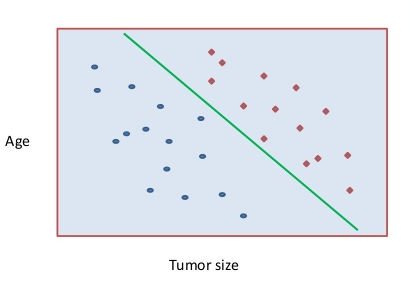
\includegraphics[width=0.9\textwidth,height=8cm]{tumor.png}
    \caption[Πρόβλημα ταξινόμησης όγκων με βάση την κακοήθεια]{Πρόβλημα ταξινόμησης όγκων με βάση την κακοήθεια}
 \end{figure}
 
\begin{itemize}
\item \textit{Χαρακτηριστικά $x_n$.} Τα στοιχεία που χαρακτηρίζουν τα δεδομένα ενός προβλήματος. Στο πρόβλημά μας κάποια χαρακτηριστικά μπορεί να είναι το μέγεθός του, το χρώμα του και η δομή του.
\item \textit{Κλάση $y_n$.} Πρόκειται για το στοιχείο που θέλουμε να προβλέψουμε, δηλαδή στην παραπάνω περίπτωση την κακοήθεια του όγκου.
\item \textit{Παραδείγματα $(x_n, y_n)$.} Τα δεδομένα του προβλήματος δίνονται συνήθως σε μορφή πίνακα: κάθε γραμμή είναι ένα παράδειγμα και οι στήλες περιέχουν τα χαρακτηριστικά και την κλάση.
\item \textit{Συνάρτηση-στόχος f. }Είναι η άγνωστη συνάρτηση που προσπαθούμε μέσω εκπαίδευσης να βρούμε. Ορίζεται ως $f : X \rightarrow Y $, στο συγκεκριμένο πρόβλημα δηλαδή καθορίζει πως προκύπτει η κακοήθεια ενός όγκου από τα χαρακτηριστικά του. Η συνάρτηση αυτή ζει στον πραγματικό κόσμο, επομένως αναμένουμε να είναι περίπλοκη, γεγονός που σε συνδυασμό με το πεπερασμένο πλήθος δεδομένων από το συγκεκριμένο χώρο περιορίζει τις προσδοκίες μας: δεν προσπαθούμε να την ορίσουμε ακριβώς, αλλά να την προσεγγίσουμε.
\item \textit{Υπόθεση h.}Το αποτέλεσμα της εκπαίδευσης, συνήθως μια ευθεία στο χώρο των χαρακτηριστικών των δεδομένων που τον χωρίζει σε 2 υποχώρους: νέα χαρακτηριστικά που φθάνουν κατατάσσονται ως κακοήθη ή καλοήθη ανάλογα με την υπόθεση. Η υπόθεση μπορεί να έχει οποιαδήποτε μορφή, ώστε να διαχωρίσει τα δεδομένα, όπως προσεγγιστικά θα έκανε και η άγνωστη συνάρτηση-στόχος.
\item \textit{Μοντέλο Εκπαίδευσης.} Προκειμένου να κάνουμε προβλέψεις σε άγνωστα δεδομένα, χρειαζόμαστε ένα μοντέλο, μία μαθηματική διαδικασία, η οποία έχει εκπαιδευθεί και παραμετροποιηθεί πάνω στο συγκεκριμένο πρόβλημα και λαμβάνοντας τα χαρακτηριστικά ενός νέου δεδομένου μπορεί να δώσει την κλάση του. Το μοντέλο αποτελείται από δύο συστατικά:
\begin{itemize}
\item \textit{Σετ υπόθεσης $H = \{h\}$.} Κάθε μοντέλο προσπαθεί να προσεγγίσει τη συνάρτηση-στόχο με διαφορετικό τρόπο. Το σετ υπόθεσης περιέχει όλες τις πιθανές υποθέσεις που μπορούν να γίνουν. Κάθε διαφορετική υπόθεση αντιστοιχεί σε διαφορετική ρύθμιση κάποιας παραμέτρου του μοντέλου και επιτελεί διαφορετική πρόβλεψη για τα δεδομένα.  Διάφορα είδη μοντέλων πρόβλεψης είναι οι perceptrons, τα νευρωνικά δίκτυα, οι μηχανές διανυσματικής στήριξης, ο ταξινομητής bayes…
\item \textit{Αλγόριθμος μάθησης.} Ανάλογα με το μοντέλο που έχουμε επιλέξει, υπάρχει μια γκάμα αλγορίθμων, οι οποίοι επιτελούν τη διαδικασία της μάθησης, προσπαθώντας να βελτιστοποιήσουν τις παραμέτρους της υπόθεσης. Για παράδειγμα οι perceptrons χρησιμοποιούν τον αλγόριθμο PLA, τα νευρωνικά τον αλγόριθμο backpropagation…
\end{itemize}
\end{itemize}
 \begin{figure}[H]
	\centering			
    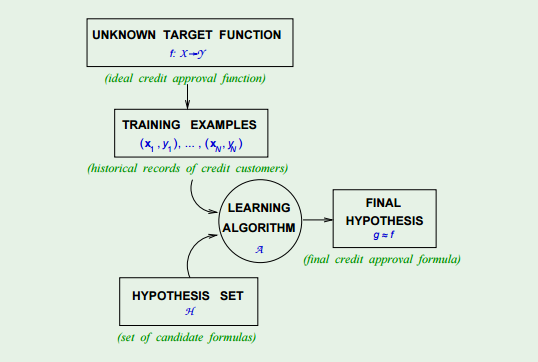
\includegraphics[width=0.9\textwidth,height=8cm]{learning.png}
    \caption[Συστατικά μηχανικής μάθησης]{Συστατικά μηχανικής μάθησης}
 \end{figure}

\subsection{Η διαδικασία της μηχανικής μάθησης}
Η παρατήρηση της διαδικασίας εφαρμογής μηχανικής μάθησης σε ένα πραγματικό πρόβλημα εξηγεί γιατί οι ειδικοί σε αυτό τον τομέα χρειάζονται ένα πλούσιο, ετερογενές επιστημονικό υπόβαθρο, εμπειρία και εφευρετικότητα. Αποτελείται από διάφορα στάδια, που αλληλοεπηρεάζονται και με βάση την αξιολόγηση επαναλαμβάνονται κατά βούληση στη διάρκεια της μάθησης.
\subsubsection{Το πρόβλημα της γενίκευσης}
Σκοπός κάθε εφαρμογής μηχανικής μάθησης είναι να κατασκευάσει ένα μοντέλο που:
\begin{itemize}
\item Προσεγγίζει κάποια άγνωστη συνάρτηση με βάση κάποια γνωστά δεδομένα με πολύ καλή ακρίβεια.
\item Μπορεί να εγγυηθεί πως δουλεύει το ίδιο καλά με άγνωστα δεδομένα.
\end{itemize}

Η πρώτη παράμετρος είναι πολύ ουσιώδης, αλλά και εύκολη να επιτευχθεί. Καθένας με στοιχειώδεις γνώσεις μαθηματικών μπορεί να σχεδιάσει μία συνάρτηση, που περνάει από όλα τα γνωστά σημεία ενός χώρου. Πώς όμως μπορούμε να αποδείξουμε πως το μοντέλο μας μπορεί να προβλέψει άγνωστα δεδομένα ή, όπως συνηθίζουμε να λέμε, μπορεί να γενικεύει; Μη έχοντας πλέον χειροπιαστά τεκμήρια, δηλαδή δεδομένα, για να στηρίξουμε τον ισχυρισμό μας, θα καταφύγουμε σε μαθηματικούς συλλογισμούς και
τεχνικές.

\paragraph{Ένα σχετικό στατιστικό πείραμα.}Έστω πως έχουμε ένα δοχείο με κόκκινους και πράσινους σβόλους. Το δοχείο είναι κλειστό, δεν μπορούμε δηλαδή να δούμε το εσωτερικό του. Αν διαλέξουμε τυχαία ένα σβώλο, τότε η πιθανότητα να είναι κόκκινος είναι $\mu$ και πράσινος $1 -\mu$.

Έστω τώρα ότι επιλέγουμε διαδοχικά ένα δείγμα από Ν σβόλους, οι οποίοι έχουν αναλογία  $\nu$ κόκκινων σβόλων. Μπορούμε, παρατηρώντας το δείγμα και την πιθανότητα $\nu$ να πούμε πως αυτή ισούται
με την άγνωστη πιθανότητα $\mu$ ;
 \begin{figure}[H]
	\centering			
    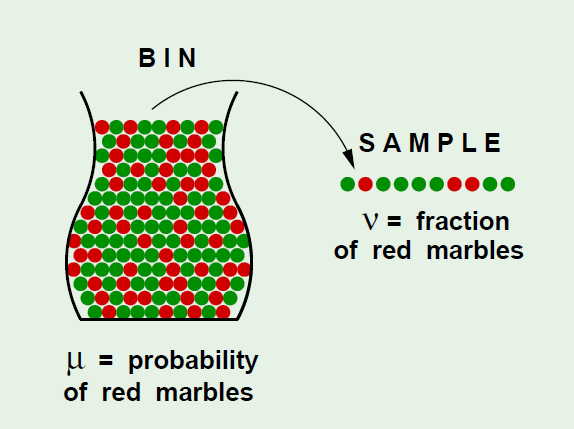
\includegraphics[width=0.9\textwidth,height=8cm]{marbles.png}
    \caption[Ένα στατιστικό πείραμα]{Ένα στατιστικό πείραμα}
 \end{figure}
 
Αν και το ενδεχόμενο οι δύο πιθανότητες να συγκλίνουν φαντάζει απίθανο, έχουμε στα χέρια μας το εξής μαθηματικό εργαλείο, που ονομάζεται ανισότητα του Hoeffding:
$$ P( \abs{ \nu-\mu} > \epsilon ) \leq 2 e ^{-2 e^2 N}$$

Η ανισότητα αυτή θέτει ένα άνω φράγμα στην απόκλιση που μπορεί να εμφανίσει η αναλογία του δείγματος από την πραγματική, δηλώνοντας πως όσο πιο μεγάλο είναι το δείγμα, τόσο πιο κοντά είναι η πιθανότητα $\nu$ στην $\mu$ .

Με όρους μηχανικής μάθησης πλέον, αν το δοχείο αντιπροσωπεύει τον άγνωστο χώρο, στον οποίο τα αντικείμενα ανήκουν σε μία από δύο κλάσεις και εγώ έχω στα χέρια μου ένα πεπερασμένο δείγμα Ν δεδομένων για το οποίο κάνω μια υπόθεση, οπότε πλέον το γεγονός ο σβόλος να είναι κόκκινος αντιστοιχεί σε σωστή υπόθεση, τότε με τη βοήθεια της ανισότητας του Hoeffding, μπορώ να ελπίζω πως αν το Ν είναι αρκούντως μεγάλο, τότε η ακρίβεια που πετυχαίνω στο δείγμα είναι κοντά στην ακρίβεια που θα πετύχω οπουδήποτε στον άγνωστο χώρο. Ωστόσο δεν έχω καταφέρει ακόμα αυτό που θέλω, καθώς στην ανισότητα έχω δύο αγνώστους: την άγνωστη πιθανότητα $\mu$ και την σταθερά $\epsilon$. Εξακολουθώ δηλαδή να μην γνωρίζω πόσο κοντά είναι η ακρίβειά μου στην ακρίβεια εκτός δείγματος.

Η λύση σε αυτό το πρόβλημα είναι απλή: αντί να προσπαθώ να παρατηρήσω την ακρίβεια στον άγνωστο χώρο, θα πάρω ένα ακόμη δείγμα μεγέθους Ν και θα μετρήσω την ακρίβεια εκεί. Αν οι ακρίβειες στα δύο δείγματα είναι κοντά, τότε μπορώ να συμπεράνω πως κοντά είναι και η ακρίβεια σε όλο το χώρο. Ο συλλογισμός είναι λογικός, αν σκεφτώ πως το νέο και το αρχικό δείγμα είναι συσχετισμένο με τον άγνωστο χώρο και άρα και μεταξύ τους. Είμαστε πλέον έτοιμοι να δούμε το πρώτο στάδιο της διαδικασίας της μηχανικής μάθησης.
\subsubsection{Διαχωρισμός σε σετ εκπαίδευσης και σετ ελέγχου}
Με το προηγούμενο πείραμα έχει γίνει εμφανής η ανάγκη ύπαρξης ενός σετ δεδομένων, ανεξάρτητου από το σετ εκπαίδευσης, αλλά στατιστικά συσχετισμένου με αυτό(καθώς και τα δύο έχουν προκύψει από την ίδια άγνωστη συνάρτηση). Το σετ εκπαίδευσης θα χρησιμοποιηθεί για την εύρεση του μοντέλου που δίνει την καλύτερη ακρίβεια για τα στοιχεία του, ενώ το σετ ελέγχου θα χρησιμοποιηθεί για να ελέγξουμε πόσο καλά δουλεύει το μοντέλο σε άγνωστα δεδομένα, ώστε να διαπιστώσουμε αν γενικεύει. Είναι πολύ σημαντικό τα 2 σετ να είναι ανεξάρτητα, δηλαδή στοιχεία του σετ ελέγχου να μην χρησιμοποιηθούν στη διαδικασία της εκπαίδευσης, όπως και στοιχεία του σετ εκπαίδευσης να μην ληφθούν υπόψιν κατά την αξιολόγηση, ειδάλλως η αξιολόγηση θα είναι πολωμένη και το σφάλμα σε πραγματικά δεδομένα αναπάντεχα μεγάλο.
\subsubsection{Εξερεύνηση δεδομένων}
Η ανάλυση των χαρακτηριστικών των δεδομένων είναι σημαντική για την κατανόηση της φύσης του προβλήματος και τη λήψη σχεδιαστικών αποφάσεων. Σε αυτή τη φάση αναγνωρίζονται κακοήθειες των χαρακτηριστικών, όπως θόρυβος, αγνοούμενες τιμές, ανιχνεύονται συσχετίσεις μεταξύ τους, αναδεικνύονται χρήσιμα χαρακτηριστικά και πρότυπα, που επηρεάζουν την καταλληλότητα των μοντέλων εκπαίδευσης. Η ανάλυση μπορεί να λάβει διάφορες μορφές, όπως τον υπολογισμό χρήσιμων μετρικών, αλλά συνήθως γίνεται μέσω οπτικοποίησης.
\begin{figure}[H]
    \centering
    \begin{minipage}{.5\textwidth}
        \centering
        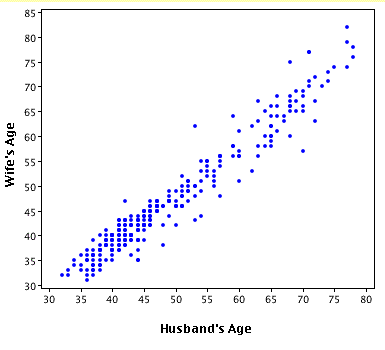
\includegraphics[width=0.8\linewidth, height=0.15\textheight]{scatter.png}
        \caption[Διάγραμμα διασποράς]{Διάγραμμα Διασποράς. Παρατηρώ πως τα χαρακτηριστικά είναι
γραμμικά συσχετισμένα}
        
    \end{minipage}%
    \begin{minipage}{0.5\textwidth}
        \centering
        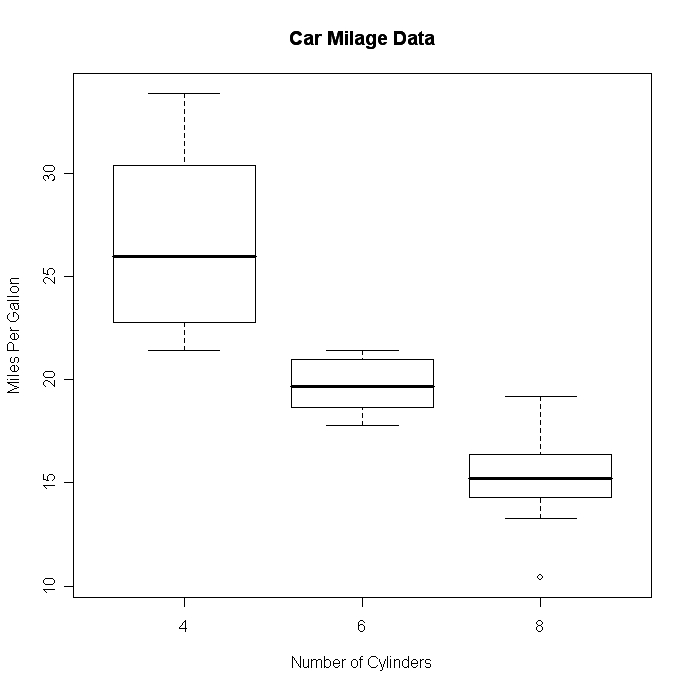
\includegraphics[width=0.8\linewidth, height=0.15\textheight]{boxplot.png}
        \caption[Θηκόγραμμα]{Θηκόγραμμα. Συνήθως χρησιμοποιείται για την ανίχνευση εξωκείμενων τιμών
και την εποπτεία της κατανομής των χαρακτηριστικών}
       
    \end{minipage}
\end{figure}

\subsubsection{Προ επεξεργασία δεδομένων}
Υπάρχουν διάφορες ενέργειες που μπορούν να εφαρμοστούν στα δεδομένα, με βάση τις ιδιαιτερότητες που παρουσιάζουν, ώστε να εξασφαλιστεί η καλή λειτουργία των αλγορίθμων μηχανικής μάθησης και εν γένει η καλή απόδοση του μοντέλου.

\paragraph{Αγνοούμενες τιμές.} Για διάφορους λόγους μπορεί να λείπουν κάποια χαρακτηριστικά από κάποιο παράδειγμα του σετ δεδομένων. Σε αυτήν την περίπτωση ο ειδικός οφείλει να επιλέξει πώς θα αντιμετωπίσει αυτήν την απώλεια πληροφορίας, καθώς οι μαθηματικοί τύποι δε δουλεύουν με άγνωστες τιμές. Ενδεχομένως να δώσει μία προκαθορισμένη τιμή σε όλα τα αγνοούμενα πεδία ή να προσπαθήσει να παρεμβάλλει την τιμή που λείπει. Σε ορισμένες περιπτώσεις μάλιστα η απουσία πληροφορίας συνιστά ένδειξη το ίδιο χρήσιμη με την απουσία της.

\paragraph{Θόρυβος} Ορισμένοι αλγόριθμοι μάθησης είναι ευαίσθητοι στο θόρυβο, ο οποίος μπορεί να αναγνωριστεί χάρις στα δομικά χαρακτηριστικά του, όπως η υψηλή διακύμανση και να αφαιρεθεί.

\paragraph{Απαγορευτικός όγκος δεδομένων.} Η υπολογιστική και χρονική πολυπλοκότητα ενός μοντέλου πρόβλεψης είναι μια ακόμη σημαντική παράμετρος, πέρα από την απόδοσή του. Η υποδειγματοληψία του σετ δεδομένων είναι μια απλή διαδικασία, που στοχεύει στη διατήρηση της πληροφορίας του αρχικού δείγματος διατηρώντας τα στατιστικά του χαρακτηριστικά.

\paragraph{Μηχανική χαρακτηριστικών.} Το κομμάτι αυτό της μηχανικής μάθησης μάλλον αποτελεί το πιο απαιτητικό και σημαντικό βήμα προς την επίτευξη ενός αποτελεσματικού μοντέλου. Ορίζεται ως η διαδικασία της μετατροπής των αρχικών, ακατέργαστων δεδομένων σε χαρακτηριστικά που αντιπροσωπεύουν καλύτερα το πρόβλημα, ώστε το μοντέλο που θα εκπαιδευτεί με αυτά να έχει καλύτερη ακρίβεια σε άγνωστα δεδομένα. Με απλά λόγια, ο μηχανικός προσπαθεί να εκμεταλλευτεί στο έπακρον τα δεδομένα, ώστε να δημιουργήσει ουσιώδη χαρακτηριστικά για το πρόβλημα που επιλύει.

Ο τρόπος με τον οποίο θα δημιουργηθούν τα χαρακτηριστικά εξαρτάται από το είδος του προβλήματος, την μορφή των δεδομένων, το μοντέλο πρόβλεψης και κινείται κυρίως στα ακόλουθα πλαίσια:
\begin{itemize}
\item \textit{Εξαγωγή χαρακτηριστικών.} Σε πολλά προβλήματα, όπως η επεξεργασία κειμένου και εικόνας, τα δεδομένα είναι τόσο πολυδιάστατα, που επίλυσή τους είναι αδύνατη. Σε αυτήν την περίπτωση υπάρχουν τεχνικές μείωσης της διαστασιμότητας, όπως η ανάλυση κυρίαρχων συστατικών, που παράγουν λιγότερα και ουσιώδη χαρακτηριστικά. Οι τεχνικές αυτές εν γένει μειώνουν τον όγκο της πληροφορίας απορρίπτοντας την περίσσειά της.
\item \textit{Δημιουργία χαρακτηριστικών.} Η διαδικασία αυτή είναι χειροκίνητη και δαπανηρή, καθώς ο ειδικός πρέπει να αναλύσει τα ακατέργαστα δεδομένα και να αναγνωρίσει δομές σε αυτά, ώστε να παράξει χαρακτηριστικά ουσιώδη για το πρόβλημα, συνδυάζοντας μεταβλητές που του δίνονται ή αναλύοντας τες. Για παράδειγμα, σε δεδομένα που δίνονται σε μορφή άρθρων, μπορεί να χρειαστεί να επισημάνει ενδεικτικές λέξεις σχετικές με το περιεχόμενο που αφορούν το πρόβλημα που επιλύει.
\item \textit{Επιλογή χαρακτηριστικών.} Αν και η επιλογή των χρήσιμων χαρακτηριστικών γίνεται από το μοντέλο εκπαίδευσης, πολύ συχνά αναγκαζόμαστε να επιλέξουμε εκ των προτέρων ένα υποσέτ των χαρακτηριστικών που μας δίνονται για διάφορους λόγους:
\begin{itemize}
\item \textit{απλοποίηση του μοντέλου για καλύτερη κατανόηση.} Σε ορισμένες εφαρμογές σκοπός μας είναι πέρα από την κατασκευή του μοντέλου, να κατανοήσουμε τον μηχανισμό που διέπει κάποιο φαινόμενο, οπότε θέλουμε να επικεντρωθούμε στα ουσιώδη χαρακτηριστικά παρά την ενδεχόμενη απώλεια στην ακρίβεια.
\item \textit{επιτάχυνση της εκπαίδευσης.} Ο χρόνος εκπαίδευσης είναι μία ακόμη παράμετρος απόδοσης ενός μοντέλου. Σε εφαρμογές που διαχειρίζονται τεράστιους όγκους δεδομένων, όπως συστήματα υπολογιστικής όρασης, η επιλογή χαρακτηριστικών είναι απαραίτητη.
\item \textit{αποφυγή υπερπροσαρμογής.} Το φαινόμενο αυτό συμβαίνει όταν προσπαθούμε πολύ να προβλέψουμε σωστά τα δεδομένα κατά την εκπαίδευση, κατασκευάζοντας ένα περίπλοκο μοντέλο, που έχει προσαρμοστεί τέλεια στις ιδιαιτερότητες του σετ εκπαίδευσης. Το μοντέλο αυτό είναι καταδικασμένο να αποτύχει σε καινούρια δεδομένα, δε γενικεύει όπως συνηθίζουμε να λέμε, καθώς έχει εκπαιδευτεί στα δεδομένα και όχι στη συνάρτηση-στόχο.
Τα βασικά κριτήρια, με τα οποία απορρίπτονται χαρακτηριστικά είναι το εξής: είτε είναι άσχετα με την κλάση, δηλαδή δεν περιέχουν πληροφορία που βοηθά στην πρόβλεψη, είτε είναι περιττά, δηλαδή η πληροφορία που περιέχουν έχει ήδη δοθεί από κάποιο άλλο χαρακτηριστικό. Σε αυτό το στάδιο συνήθως χρησιμοποιούνται τεχνικές φιλτραρίσματος, οι οποίες υπολογίζουν τη συσχέτιση των χαρακτηριστικών με τη κλάση και τις συσχετίσεις μεταξύ των χαρακτηριστικών και επιλέγουν υποσύνολα με τη χρήσιμη πληροφορία. Θα δούμε στη συνέχεια ότι υπάρχουν και άλλες τεχνικές επιλογής χαρακτηριστικών.
\end{itemize}
\end{itemize}
 \begin{figure}[H]
	\centering			
    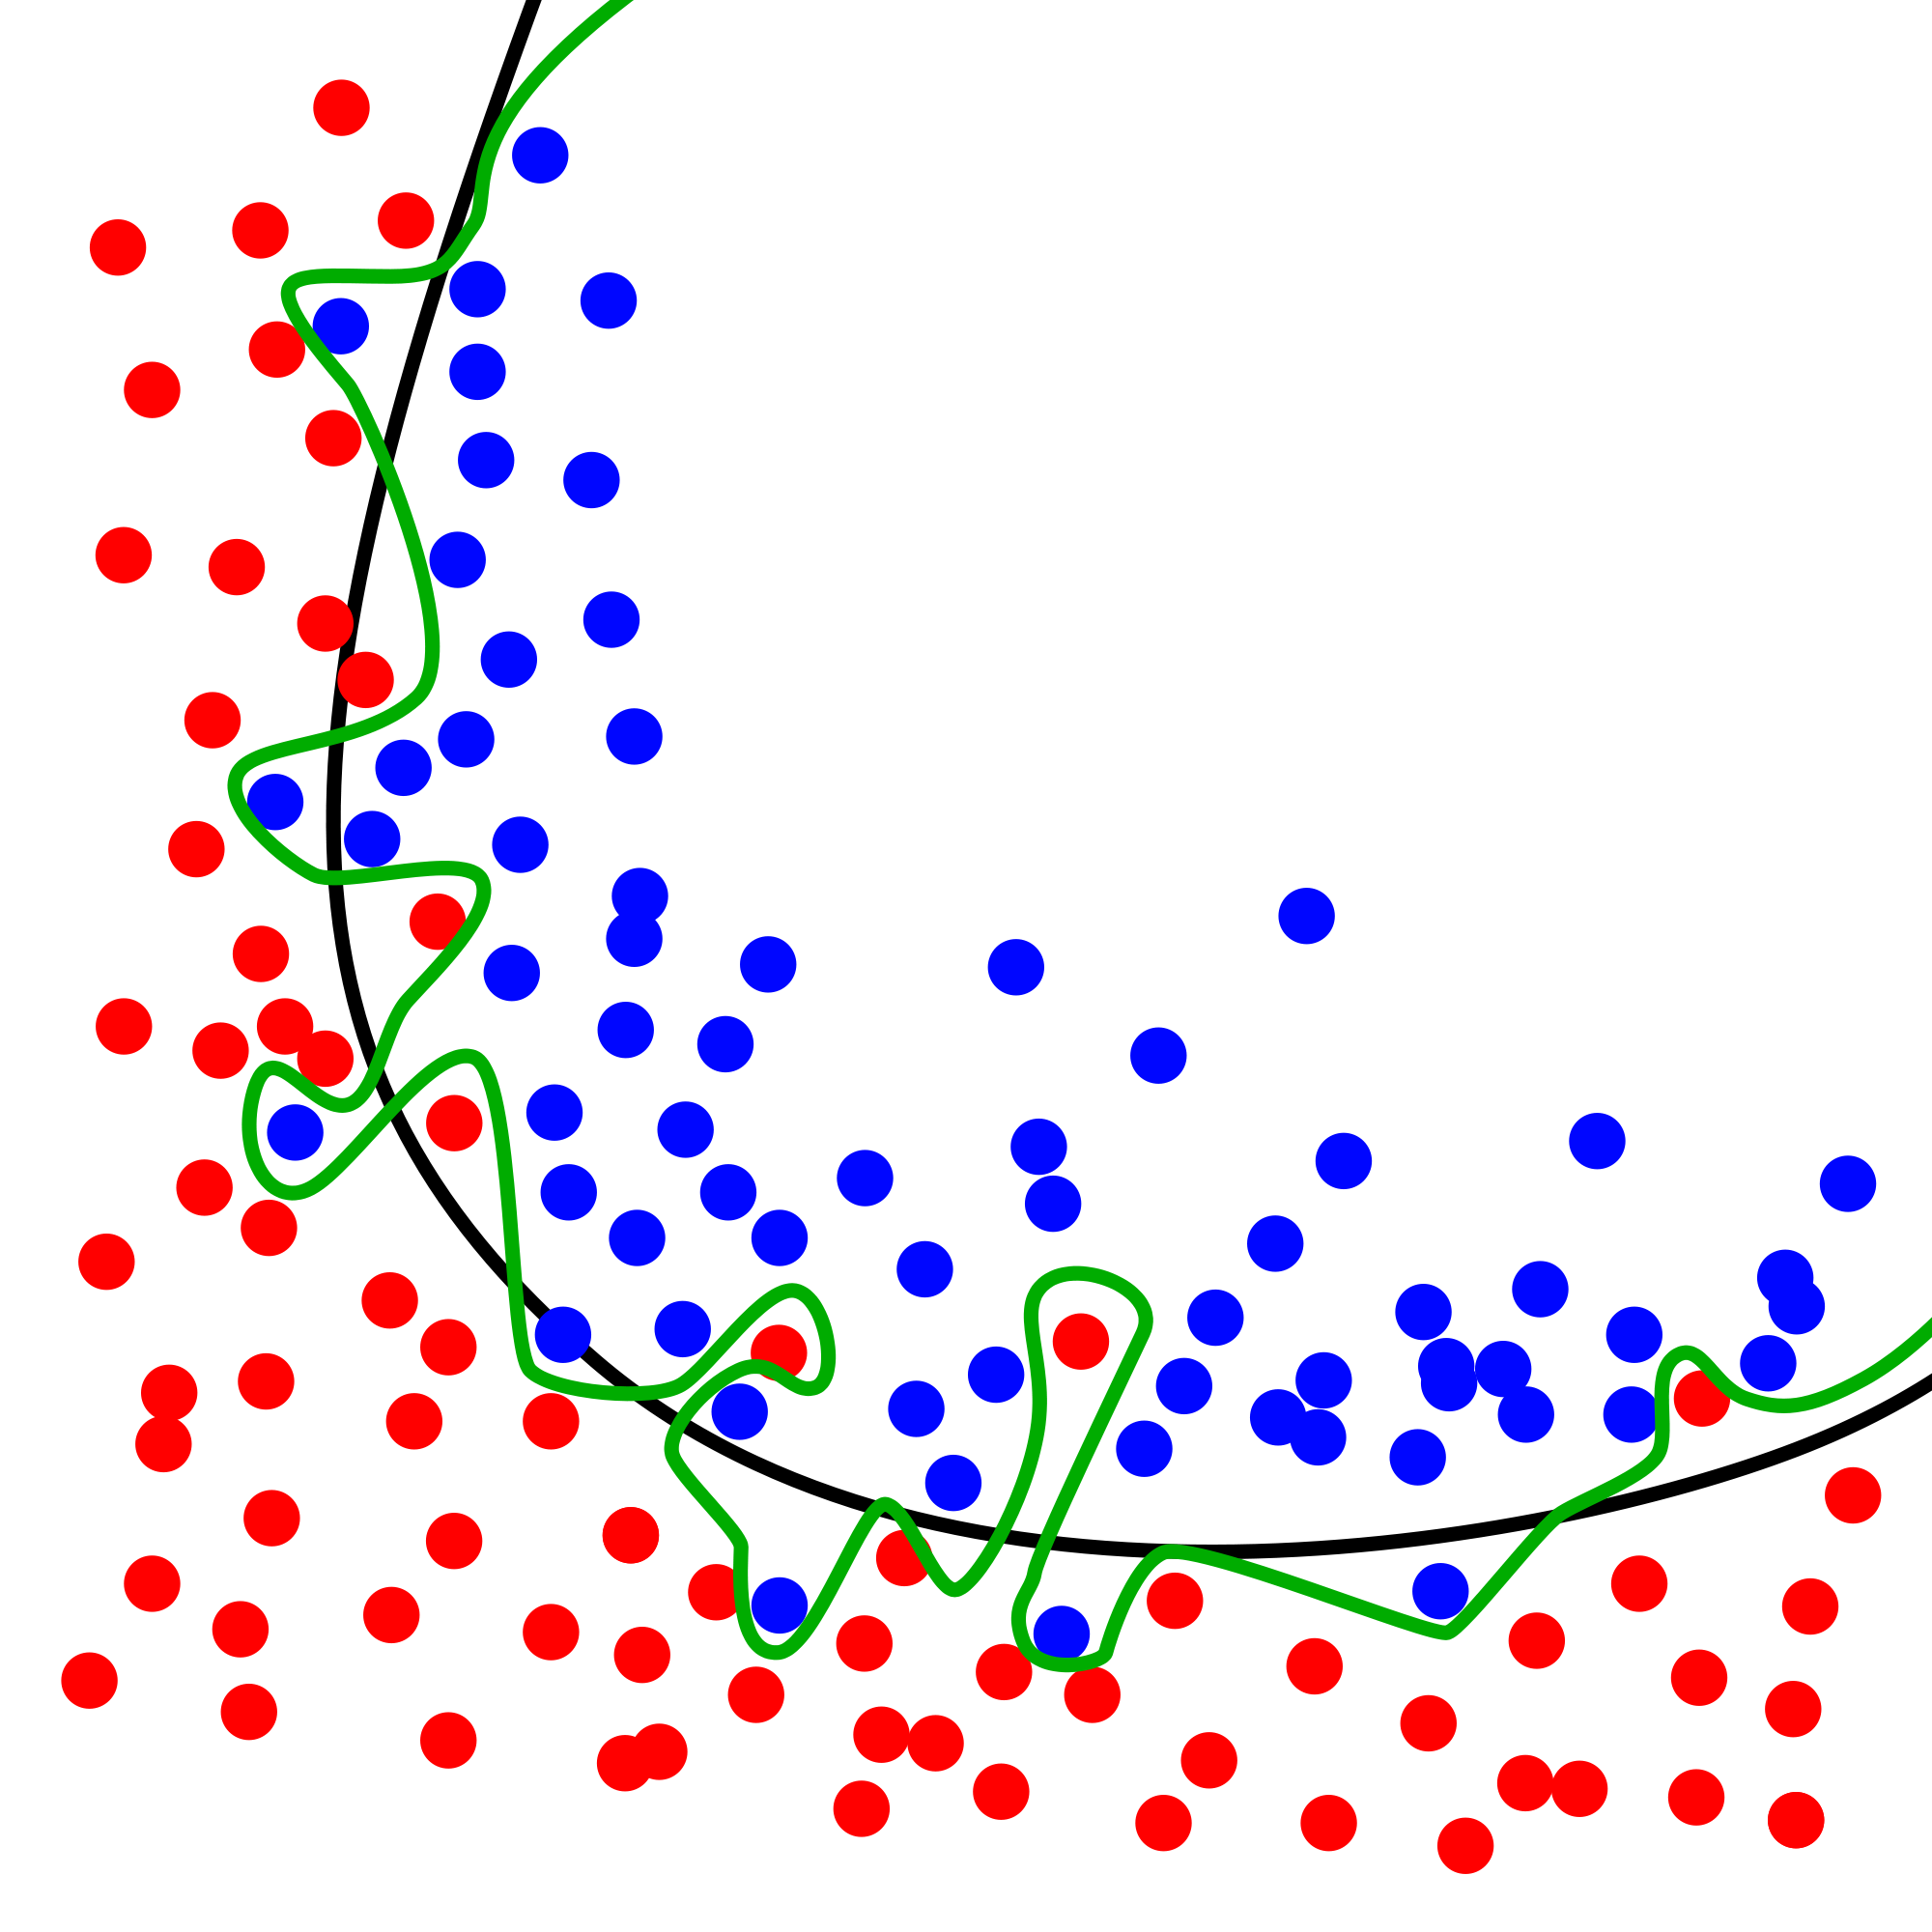
\includegraphics[width=0.7\textwidth, height=7cm]{overfit.png}
    \caption[Το πρόβλημα της υπερπροσαρμογής]{Το πρόβλημα της υπερπροσαρμογής: το μοντέλο χαρακτηρίζεται από περίπλοκη υπόθεση (πράσινη γραμμή), καθώς έχει γίνει η προσπάθεια να προβλεπτούν σωστά όλα τα δεδομένα εκπαίδευσης. Η πραγματική συνάρτηση (μαύρο χρώμα) είναι απλούστερη και παραβιάζεται για κάποια δεδομένα χαμηλής ποιότητας.}
 \end{figure}

\paragraph{Ανισορροπία κλάσης.} Σε πολλά πραγματικά προβλήματα η κλάση που προβλέπουμε έχει σπάνια συχνότητα εμφάνισης. Για παράδειγμα σε μία εφαρμογή ανίχνευσης εξαπάτησης σε οικονομικές συναλλαγές, τα παραδείγματα εξαπάτησης θα είναι πολύ λιγότερα, καθώς οι τράπεζες διαθέτουν δικλίδες ασφαλείας για την αποφυγή τους. Ένας ταξινομητής λοιπόν που θα εκπαιδευθεί σε ένα ανισόρροπο σετ
εκπαίδευσης, θα μάθει να προβλέπει καλά παραδείγματα μόνο της μίας κλάσης.

Ας συνεχίσουμε με αυτό το ακραίο, αλλά κατατοπιστικότατο παράδειγμα. Έστω ότι για την εφαρμογή ανίχνευσης εξαπάτησης που αναφέραμε, έχουμε $10000$ παραδείγματα, εκ των οποίων τα $9990$ αντιστοιχούν σε νόμιμη συναλλαγή και τα $10$ σε εξαπάτηση. Τότε, αν εκπαιδεύσουμε έναν ταξινομητή με στόχο την σωστή ανίχνευση όσο περισσότερων παραδειγμάτων γίνεται, τότε ένας μοντέλο που προβλέπει
όλες τις συναλλαγές ως νόμιμες θα καταφέρει να κατατάξει σωστά το $ 99 \%$ των παραδειγμάτων. Μη λαμβάνοντας λοιπόν υπόψιν την ανισορροπία των δεδομένων, έχουμε παραπλανηθεί προς τη δημιουργία ένα πολύ κακού μοντέλου.

Ευτυχώς η αντιμετώπιση του προβλήματος αυτού είναι πολύ εύκολη και μπορεί να γίνει με:
\begin{itemize}
\item \textit{επιβολή κόστους στην λανθασμένη κατηγοριοποίηση της σπάνιας κλάσης.} Αλγόριθμοι όπως οι μηχανές διανυσματικής στήριξης, που ενσωματώνουν την έννοια του κόστους, μπορούν να τροποποιηθούν ώστε να παίρνουν μεταβλητά κόστη για τις διάφορες κλάσεις. Έτσι, ακόμη κι αν λόγω μικρού πλήθους παραδειγμάτων κάνουμε λίγα σφάλματα, αυτά θα έχουν μεγάλη βαρύτητα.
\item \textit{δειγματοληψία.} Αν υποδειγματοληπτήσουμε την κλάση πλειοψηφίας και υπερδειγματοληπτήσουμε την σπάνια κλάση, μπορούμε να εξισορροπήσουμε τη συχνότητα εμφάνισης των κλάσεων. Αυτή η τεχνική ενέχει ωστόσο κινδύνους: μπορεί να πετάξουμε χρήσιμη πληροφορία από τη κλάση πλειοψηφίας, αλλοιώνοντας την αντίληψη που έχουμε για το πρόβλημα, αλλά και να υπερεκπαιδευτούμε στα συγκεκριμένα παραδείγματα της σπάνιας κλάσης, χωρίς να κερδίσουμε κάτι από άποψη γενίκευσης.
\item \textit{συνθετική τεχνική υπερδειγματοληψίας της κλάσης μειοψηφίας (SMOTE).} Πρόκειται για μια πρόσφατη, απλή και αποτελεσματική τεχνική, που συνδυάζει υπό- και υπερδειγματοληψία, δίνοντας ιδιαίτερη έμφαση στη δεύτερη: αντί να επαναλαμβάνει απλά τα παραδείγματα με σπάνια κλάση, προσπαθεί να δημιουργήσει νέα μέσω ενός απλού αλγορίθμου:
\end{itemize}
\begin{myalgorithm}[H]

 \For{c ανήκει στην σπάνια κλάση }{
  βρες τους 5 κοντινότερος γείτονες\;
  διάλεξε τυχαία έναν n\;
  Δημιούργησε ένα νέο παράδειγμα r με βάση τα χαρακτηριστικά feats των n και c ως εξής:\;
 r.feats=c.feats + (c.feats -n.feats) * rand(0,1) \;
 }
 \caption{SMOTE}
\end{myalgorithm}

\paragraph{Κανονικοποίηση.} Τα χαρακτηριστικά σε ένα πρόβλημα ταξινόμησης κινούνται σε διαφορετικά εύρη τιμών: σε μία εφαρμογή που μελετά τα χαρακτηριστικά μιας οικογένειας, το πλήθος των μελών κυμαίνεται σε πολύ διαφορετικές τιμές από το εισόδημα. Τα περισσότερα μοντέλα υπολογίζουν αποστάσεις μεταξύ των παρατηρήσεων με χρήση της ευκλείδειας απόστασης, που είναι ευαίσθητη στα μέτρα των επιμέρους χαρακτηριστικών. Προκειμένου λοιπόν να εξασφαλίσουμε πως ο αλγόριθμος δε θα επηρεαστεί, οφείλουμε να εξασφαλίσουμε πως τα χαρακτηριστικά κινούνται στο ίδιο εύρος . Δύο είναι οι βασικές τεχνικές κανονικοποίησης:
\begin{flalign*}
\text{Επανακλιμάκωση} && x^, & =\frac{ x - \min{x}}{\max{x} - \min{x}} &&
\end{flalign*}
ώστε τα χαρακτηριστικά να κυμαίνονται στο εύρος $[0,1]$
\begin{flalign*}
\text{Τυποποίηση} && x^, & =\frac{ x - \bar{x}}{\sigma} &&
\end{flalign*}
ώστε τα χαρακτηριστικά να έχουν μηδενική μέση τιμή και μοναδιαία διακύμανση

\subsubsection{Εκπαίδευση μοντέλου}
Το πιο αναγνωρίσιμο μάλλον στάδιο της μηχανικής μάθησης είναι αυτό της εκπαίδευσης του μοντέλου. Εδώ, ο ειδικός διαλέγει το σετ υποθέσεων που θα δοκιμάσει και τον αλγόριθμο μάθησης και χρησιμοποιώντας τα δεδομένα που έχει στο σετ εκπαίδευσης κατασκευάζει το μοντέλο πρόβλεψης. Αν και η διαδικασία είναι αυτοματοποιημένη, υπάρχουν κάποιες επιλογές που επηρεάζουν το αποτέλεσμα και μπορούν να γίνουν είτε τυχαία είτε προς όφελός του.

\paragraph{Επιλογή χαρακτηριστικών.} Αν και συναντήσαμε την επιλογή χαρακτηριστικών κατά την προ επεξεργασία των δεδομένων, θα την επαναλάβουμε και σε αυτό το στάδιο, με διαφορετικό όμως σκοπό. Έχουμε ήδη αφαιρέσει την περίσσεια πληροφορίας, που δε θα προσέφερε κάτι στη μάθηση, χωρίς όμως αυτό να σημαίνει πως όλα τα χαρακτηριστικά που χρησιμοποιούμε είναι χρήσιμα. Αυτό οφείλεται στο γεγονός ότι παρατηρήσαμε μόνο τα στατιστικά χαρακτηριστικά των δεδομένων, χωρίς να ασχοληθούμε με την κλάση. Σε αυτό το στάδιο έχουμε τη δυνατότητα να εκπαιδεύσουμε το μοντέλο μας με διαφορετικά υποσύνολα των χαρακτηριστικών και να αξιολογήσουμε τις ακρίβειες των διαφορετικών μοντέλων, ώστε να συμπεράνουμε ποια χαρακτηριστικά συνεισφέρουν σίγουρα στην πρόβλεψη. Οι μέθοδοι που το επιχειρούν αυτό λέγονται wrapper, επειδή εμπλέκουν και τη διαδικασία της εκπαίδευσης και είναι σαφέστατα πιο αποδοτικοί από τις μεθόδους φιλτραρίσματος που είδαμε, καθώς λαμβάνουν αποφάσεις πολύ πιο συνειδητά.
\begin{figure}[H]
	\centering			
    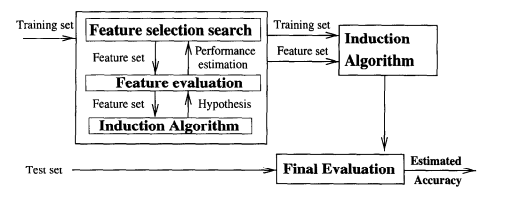
\includegraphics[width=0.9\textwidth]{wrapper.png}
    \caption[Μέθοδος Wrapper για επιλογή χαρακτηριστικών]{Μέθοδος Wrapper για επιλογή χαρακτηριστικών}
 \end{figure}
 
 Στο παραπάνω σχήμα βλέπουμε πως οι μέθοδοι αυτοί διαλέγουν διαδοχικά ένα υποσύνολο των χαρακτηριστικών, εκπαιδεύουν ένα μοντέλο, το αξιολογούν και στη συνέχεια παραδίδουν το μοντέλο με την καλύτερη απόδοση και τα χαρακτηριστικά που επέλεξαν. Είναι σημαντικό πως κατά την επαναληπτική διαδικασία της επιλογής χαρακτηριστικών, η εκπαίδευση και η αξιολόγηση γίνεται σε $2$ διαφορετικά υποσύνολα του σετ εκπαίδευσης. Συνήθως χρησιμοποιούμε τα $9/10$ του σετ για εκπαίδευση και το $1/10$ για την αξιολόγηση (το υποσύνολο αυτό συνηθίζουμε να το αποκαλούμε σετ αξιολόγησης). Ο λόγος του διαχωρισμού είναι ο ίδιος που οδήγησε στο σχηματισμό του σετ εκπαίδευσης και ελέγχου: αν εκπαιδεύαμε το μοντέλο σε κάποια παραδείγματα με ένα υποσύνολο των χαρακτηριστικών και αξιολογούσαμε την απόδοση του μοντέλου στα ίδια παραδείγματα, τότε θα διαλέγαμε τα κυρίαρχα χαρακτηριστικά με βάση μόνο αυτά, διακυβεύοντας τη γενίκευση του μοντέλου.
 
 Η λογική με την οποία επιλέγονται τα υποσύνολα που θα δοκιμαστούν ακολουθεί συνήθως μία από δύο διαφορετικές συλλογιστικές:
 \begin{itemize}
 \item \textit{προς τα εμπρός επιλογή.} Ξεκινά με ένα άδειο σύνολο και προσθέτει διαδοχικά χαρακτηριστικά που μειώνουν το σφάλμα ταξινόμησης μέχρι καμία προσθήκη να μη το βελτιώνει.
 \item \textit{προς τα πίσω επιλογή.} Ξεκινά με όλα τα χαρακτηριστικά και αφαιρεί διαδοχικά χαρακτηριστικά που μειώνουν το σφάλμα ταξινόμησης μέχρι καμία αφαίρεση να μη το βελτιώνει.
 \end{itemize}
 Τα βασικά μειονεκτήματα αυτών των μεθόδων είναι πως είναι χρονοβόρα και μπορεί να οδηγήσουν σε υπερπροσαρμογή.
 
 \paragraph{Βελτιστοποίηση υπερπαραμέτρων.} Κάθε μοντέλο ταξινόμησης χαρακτηρίζεται από κάποιες παραμέτρους, οι οποίες ρυθμίζονται από τους αλγόριθμους εκμάθησης κατά την εκπαίδευση, και κάποιες υπερπαραμέτρους, που δεν ορίζουν άμεσα την υπόθεση, ωστόσο την επηρεάζουν. Για παράδειγμα, όταν προσεγγίζουμε το ελάχιστο κάποια συνάρτησης υπάρχουν παράμετροι που καθορίζουν το βήμα με το οποίο κινούμαστε και επομένως έχουν επίπτωση στην ταχύτητα, αλλά και την επιτυχία της σύγκλισης. Άλλοι παράμετροι καθορίζουν πόσο ελαστικό είναι το μοντέλο στη λανθασμένη ταξινόμηση κάποιων χαρακτηριστικών, με κύριο μέλημα την αποφυγή υπερπροσαρμογής.
 
 Η επιλογή των υπερπαραμέτρων αυτών πρέπει να γίνει λοιπόν από τον ειδικό και είναι γεγονός πως η διαισθητική βελτιστοποίησή τους είναι δύσκολη, λόγω της πολυπλοκότητας της εμπλοκής τους στους αλγορίθμους. Ακόμη, αν οι υπερπαράμετροι επιλεγούν τυχαία, τότε ο αλγόριθμος εκμάθησης θα βελτιστοποιήσει τις παραμέτρους της υπόθεσης, το μοντέλο όμως θα είναι κατά πάσα περίπτωση υποβέλτιστο.
 
 Ο συνήθης τρόπος αναζήτησης των βέλτιστων υπερπαραμέτρων είναι σε ένα πλέγμα: ο ειδικός επιλέγει κάποιες πιθανές τιμές, που θεωρεί αποδεκτές για κάθε υπερπάραμετρο που επηρεάζει το μοντέλο και στη συνέχεια για κάθε συνδυασμό τιμών εκπαιδεύει και αξιολογεί ένα μοντέλο. Έχοντας εξαντλήσει τις επιλογές του, επιλέγει τις τιμές των υπερπαραμέτρων που είχαν την καλύτερη απόδοση.
 
 \subsubsection{Αξιολόγηση μοντέλου}
 Το τελευταίο στάδιο της διαδικασίας της μηχανικής μάθησης είναι αυτό της αξιολόγησης της ποιότητας του μοντέλου, όρου αφηρημένου, που παίρνει υπόσταση με βάση την εφαρμογή και τη διατύπωση του προβλήματος. Στη συνέχεια θα δούμε κάποιες μετρικές και γραφικούς τρόπους απεικόνισης της απόδοσης ενός μοντέλου.
 
 \paragraph{Μετρικές αξιολόγησης μοντέλου.} Οι μετρικές προκύπτουν από τον πίνακα σύγχυσης ενός ταξινομητή, ο οποίος συνοψίζει την πληροφορία για το πόσα παραδείγματα από κάθε κλάση ταξινομήθηκαν σωστά. Η μορφή του φαίνεται στην παρακάτω εικόνα:
 \begin{figure}[H]
	\centering			
    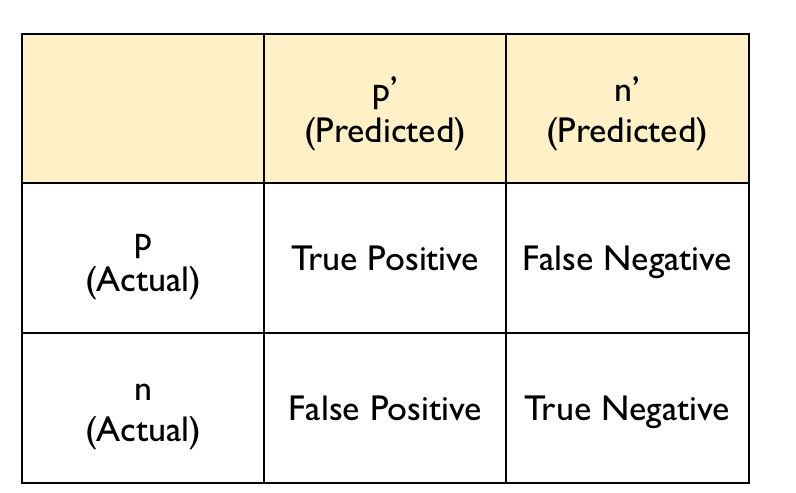
\includegraphics[width=0.6\textwidth, height=5cm]{confusion.png}
    \caption[Πίνακας σύγχυσης ταξινομητή ]{Πίνακας σύγχυσης ταξινομητή}
 \end{figure}
\begin{flalign*}
\text{Ακρίβεια} & =\frac{ TruePositive + TrueNegative}{TruePositive + TrueNegative + FalseP ositive + FalseNegative}  &\\
\text{Ακρίβεια (Precision)} & =\frac{TruePositive}{TruePositive + FalsePositive}  &\\
\text{Ανάκληση} , & =\frac{ TruePositive}{TruePositive + FalseNegative}  &\\
\text{Μετρική F}  & =\frac{ 2 \cdot TruePositive}{2 \cdot TruePositive + FalseP ositive + FalseNegative }  &\\
\end{flalign*} 

\paragraph{Γραφική απεικόνιση απόδοσης μοντέλου- Καμπύλες ROC.} Οι καμπύλες αυτές δείχνουν πόσο καλά δουλεύει ένας δυαδικός ταξινομητής, ο οποίος υπολογίζει μία συνεχή τιμή για κάθε παράδειγμα και το αναθέτει στη θετική κλάση, αν αυτή η τιμή ξεπερνά κάποιο κατώφλι, ειδάλλως στην αρνητική. Το διάγραμμα σχηματίζεται βάζοντας ένα σημείο για κάθε διαφορετική τιμή κατωφλίου με τετμημένη το FPR και τεταγμένη το TPR, όπου:
\begin{flalign*}
\text{TPR}&=\frac{ TruePositive}{TruePositive + FalseNegative}  && \text{και}  && FPR=\frac{FalsePositive}{FalsePositive + TrueNegative} 
\end{flalign*}
 \begin{figure}[H]
	\centering			
    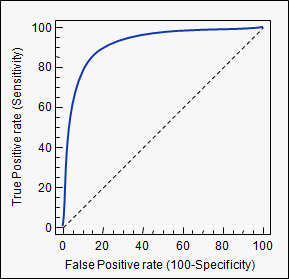
\includegraphics[width=0.6\textwidth, height=6cm]{roc.png}
    \caption[Roc καμπύλη ταξινομητή]{Roc καμπύλη ταξινομητή}
 \end{figure}
 
 Μερικά ποιοτικά συμπεράσματα που μπορούμε να βγάλουμε κοιτώντας τη ROC καμπύλη είναι τα εξής:
 \begin{itemize}
 \item όσο πιο αριστερά και πάνω βρισκόμαστε, τόσο καλύτερη είναι η ταξινόμηση.
 \item η ευθεία $y = x$ αντιστοιχεί σε τυχαίο ταξινομητή.
 \item μπορώ να συγκρίνω δύο ταξινομητές κοιτώντας το εμβαδό της περιοχής κάτω από τη καμπύλη: μεγαλύτερο εμβαδό αντιστοιχεί σε καλύτερο ταξινομητή.
 \end{itemize}
 \section{Τεχνικές μηχανικής μάθησης}
 \subsection{Μοντέλα ταξινόμησης}
 Σε αυτό το κεφάλαιο θα γνωρίσουμε διάφορα μοντέλα ταξινόμησης προσπαθώντας να καλύψουμε τις σημαντικότερες οικογένειες αλγορίθμων, ώστε να αντιληφθούμε την ποικιλομορφία των τεχνικών που μπορούν να εφαρμοστούν σε ένα πρόβλημα μηχανικής μάθησης. Θα ξεκινήσουμε με την απλή οικογένεια των αλγορίθμων βασισμένων σε παραδείγματα, θα περάσουμε στους πιθανοτικούς και τελικά θα κατανοησούμε τη λειτουργία δύο σημαντικών, για διαφορετικούς λόγους, μοντέλων: των νευρωνικών δικτύων και των
μηχανών διανυσματικής στήριξης. 
\subsubsection{Κ-κοντινότερος γείτονας}
Ο αλγόριθμος αυτός ανήκει στην κατηγορία των αλγορίθμων  αλγορίθμων βασισμένων σε παραδείγματα, δηλαδή οι προβλέψεις του βασίζονται εξ ολοκλήρου στα παραδείγματα (instances) και δε λαμβάνει χώρα κάποια εκπαίδευση. Οι αλγόριθμοι αυτοί είναι πολύ χρήσιμοι σε εφαρμογές που απαιτούν online μάθηση, επειδή τα δεδομένα έρχονται σειριακά και δεν είναι διαθέσιμα σε ομάδες για εκπαίδευση, όπως σε προβλέψεις μετοχών στο χρηματιστήριο.

Αν φανταστούμε πως τα δεδομένα ζουν σε ένα χώρο ίσων διαστάσεων με το πλήθος των χαρακτηριστικών και διαφοροποιούνται ως προς την κλάση τους, τότε η ταξινόμηση ενός σημείου με άγνωστη κλάση γίνεται ως εξής: βρίσκουμε τους k κοντινότερους γείτονές του και του αναθέτουμε την κλάση της πλειοψηφίας.
 \begin{figure}[H]
	\centering			
    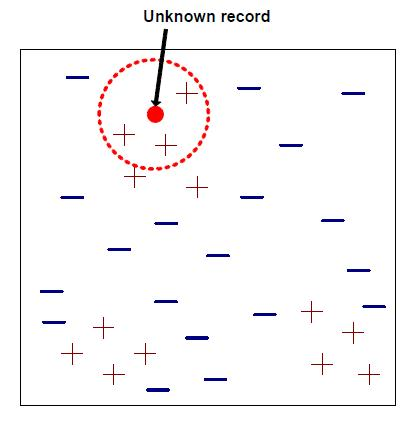
\includegraphics[width=0.6\textwidth, height=6cm]{knn.png}
    \caption[K-NN ταξινομητής]{K-NN ταξινομητής: Το άγνωστο σημείο θα ταξινομηθεί ως θετικό.}
 \end{figure}
 Μία σημαντική παράμετρος, που εξαρτάται από το πεδίο εφαρμογής, είναι ο τρόπος με τον οποίο υπολογίζεται η απόσταση μεταξύ των σημείων. Διάφορες επιλογές είναι:
 \begin{itemize}
 \item \textit{Ευκλείδεια απόσταση.} Πρόκειται για το συνηθέστερο τρόπο υπολογισμού απόστασης και δίνεται από τον τύπο:
 $$\sqrt[]{\sum_{i=1}^{Κ} (x_i - y_i )^2}$$
 \item \textit{Απόσταση Hamming.} Χρησιμοποιείται για κατηγορικά δεδομένα και κυρίως σε εφαρμογές επεξεργασίας κειμένου. Η απόσταση μεταξύ δύο παραδειγμάτων είναι το άθροισμα της απόστασης μεταξύ των χαρακτηριστικών τους, που ισούται με μηδέν για τα χαρακτηριστικά που συμπίπτουν και ένα για τα υπόλοιπα.
  \item \textit{Απόσταση Manhattan.} Εμπνευσμένη από την οργάνωση του Manhattan σε οικοδομικά τετράγωνα, για τον υπολογισμό της απόστασης μεταξύ δύο σημείων μπορούμε να κινηθούμε μόνο οριζοντίως ή καθέτως. Ορίζεται ως εξής:
  $$\sum_{i=1}^{Ξ} \abs{x_i - y_i}$$
 \end{itemize}
 
 Τέλος, η επιλογή του k οφείλει να γίνει με προσοχή. Αν είναι πολύ μεγάλο υπάρχει ο κίνδυνος κατά την ταξινόμηση να λαμβάνουμε υπόψιν πολύ μακρινά παραδείγματα, ενώ αν είναι πολύ μικρό η ταξινόμηση θα επηρεάζεται εύκολα από ενδεχόμενο θόρυβο στα δεδομένα.
\subsubsection{Συνάρτηση Ακτινικής βάσης }
Η συνάρτηση αυτή σχετίζεται με πολλές έννοιες της μηχανικής μάθησης. Σε αυτό το σημείο θα ορίσουμε το βασικό της μοντέλο και θα δούμε τη λειτουργία της ως τεχνική βασισμένη σε παραδείγματα. 

Η λογική του  μοντέλου αυτού είναι η εξής: η υπόθεση σε ένα σημείο επηρεάζεται από την απόστασή του από κάθε παράδειγμα του σετ εκπαίδευσης. Πιο συγκεκριμένα, η μαθηματική διατύπωση της υπόθεσης, που έχει και τη μορφή του σχήματος που ακολουθεί, είναι η εξής:
$$h(x)= sign( \sum_{n=1}^{N} w_n e^{-\gamma \norm{x - x_n}^2})$$
\begin{figure}[H]
	\centering			
    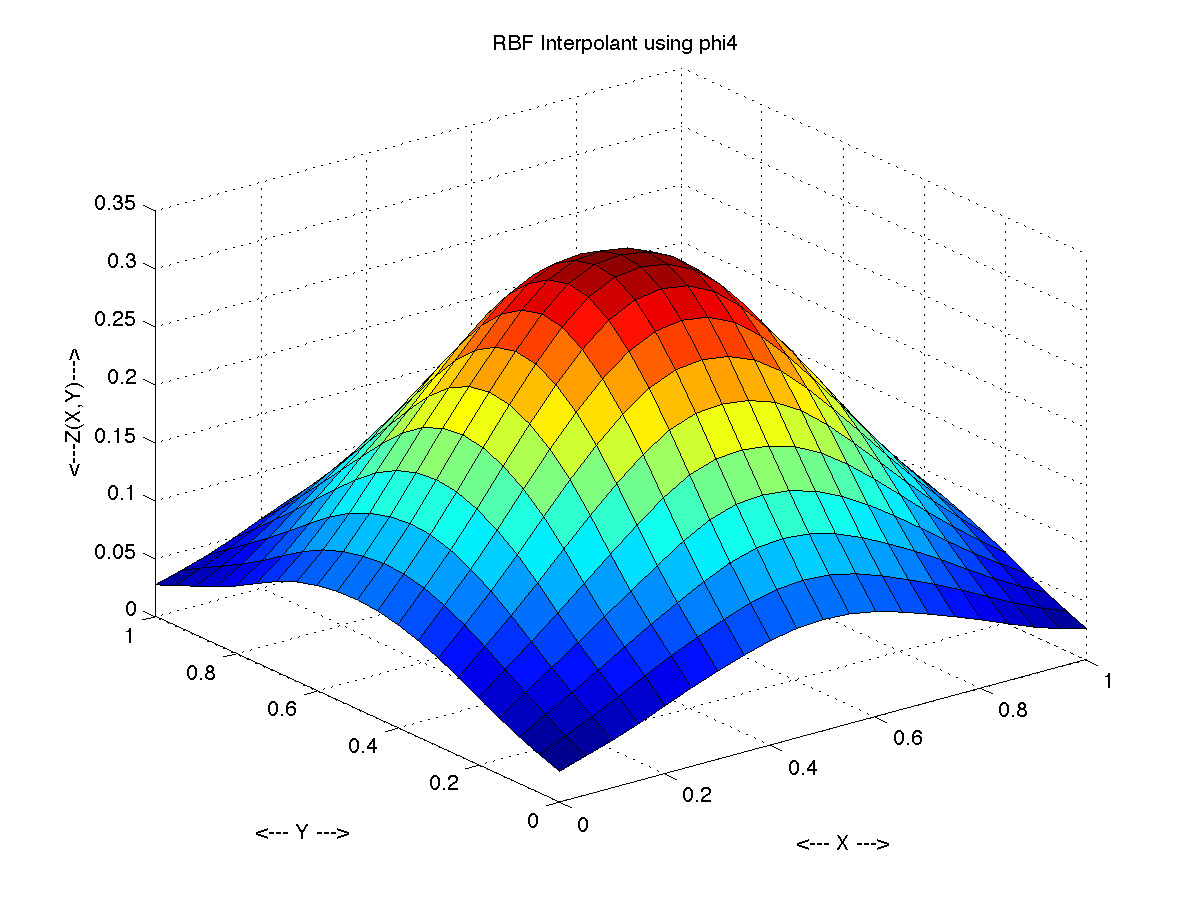
\includegraphics[width=0.6\textwidth]{rbf.png}
    \caption[Radial Basis συνάρτηση με γκαουσιανή βάση]{Radial Basis συνάρτηση με γκαουσιανή βάση.}
 \end{figure}
 Η επιλογή της βέλτιστης υπόθεσής έγκειται σε αυτήν που προβλέπει σωστά όλα τα παραδείγματα του σετ εκπαίδευσης. Αν και συνήθως προσπαθούμε να ελαχιστοποιήσουμε το σφάλμα, εδώ είμαστε σίγουροι πως θα καταφέρουμε να το μηδενίσουμε, καθώς το μοντέλο μας έχει στη διάθεση του πάρα πολλές παραμέτρους (όσα είναι και τα παραδείγματα). Επομένως το πρόβλημα βελτιστοποίησης ορίζεται ως:
 $$E_{in}=0 \rightarrow  \sum_{n=1}^{N} w_n e^{-\gamma \norm{x_n - x_m}^2}= y_n  \forall n \in D_N $$
 όπου $E_{in}$ είναι το σφάλμα στα παραδείγματα εκπαίδευσης και$ D_N$ το σετ εκπαίδευσης. 
 
 Ο παραπάνω τύπος δίνει ένα σύστημα Ν γραμμικών εξισώσεων με Ν αγνώστους που διατυπώνεται εύκολα ως εξής:
 \[
 \underbrace{
\begin{bmatrix}
    e^{-\gamma \norm{x_1 - x_1}^2}  & \dots  &  e^{-\gamma \norm{x_1 - x_N}^2} \\
     e^{-\gamma \norm{x_2 - x_1}^2}  & \dots  &  e^{-\gamma \norm{x_2 - x_N}^2} \\
    \vdots  & \vdots & \vdots \\
     e^{-\gamma \norm{x_N - x_1}^2}  & \dots  &  e^{-\gamma \norm{x_N - x_N}^2} \\
\end{bmatrix}}_{  \Phi}
\underbrace{
\begin{bmatrix}
    w_{1}       \\
    w_{2}        \\
    \vdots        \\
    w_{N}
\end{bmatrix}}_{W}
=
\underbrace{
\begin{bmatrix}
    y_{1}       \\
    y_{2}        \\
    \vdots        \\
    y_{N}
\end{bmatrix}}_{Y}
\]

Η λύση αυτού του συστήματος δίνεται από τον τύπο:
$$w=\inv{\Phi} y$$
όπου ο πίνακας $\Phi$ πρέπει να είναι αντιστρέψιμος

\paragraph{Επίδραση της μεταβλητής γ} Η μεταβλητή αυτή ορίζει πόσο απλωμένη είναι η καμπάνα γύρω από κάθε σημείο του σετ εκπαίδευσης και άρα πόσο επίδραση έχει αυτό στη γειτονιά του.
\begin{figure}[H]
    \centering
    \begin{minipage}{.5\textwidth}
        \centering
        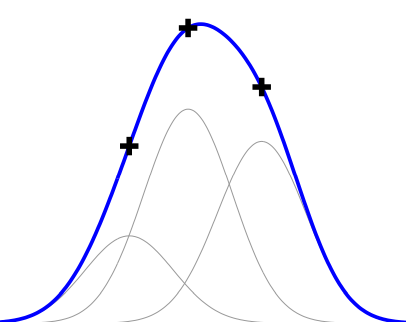
\includegraphics[width=0.8\linewidth, height=0.15\textheight]{smallg.png}
        \caption[RBF με μικρό γ]{RBF με μικρό γ}
        
    \end{minipage}%
    \begin{minipage}{0.5\textwidth}
        \centering
        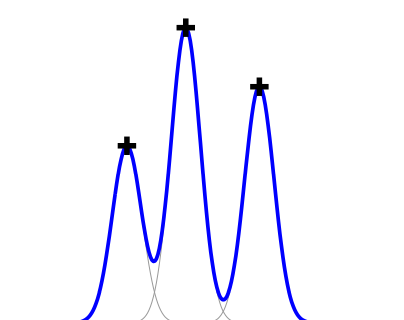
\includegraphics[width=0.8\linewidth, height=0.15\textheight]{big.png}
        \caption[RBF με μεγάλο γ]{RBF με μεγάλο γ}
       
    \end{minipage}
\end{figure}
\paragraph{H συνάρτηση RBF ως μοντέλο βασισμένο σε παραδείγματα.} Όπως είδαμε η ταξινόμηση ενός σημείου εξαρτάται από την απόστασή του από τα υπόλοιπα του σετ εκπαίδευσης, τεχνική που παραπέμπει άμεσα στη λογική της κατηγοριοποίησης με βάση τα παραδείγματα. Μέχρι τώρα έχουμε θεωρήσει ως συνάρτηση βάσης την γκαουσιανή, αν όμως τοποθετήσουμε έναν απλό κύλινδρο γύρω από κάθε σημείο, η τεχνική αυτή ταυτίζεται με το μοντέλο k-
NN .
\paragraph{Επιλογή Κ κέντρων.} Η χρήση τόσων παραμέτρων όσων είναι και τα στοιχεία του σετ εκπαίδευσης κάνει τη διαδικασία της εκπαίδευσης χρονοβόρα και ενέχει κινδύνους υπερπροσαρμογής. Συνήθως λοιπόν χρησιμοποιούμε μια τροποποίηση της τεχνικής που έχουμε περιγράψει, όπου αντί να υπολογίζουμε την απόσταση από όλα τα σημεία, επιλέγουμε Κ αντιπροσωπευτικά σημεία του χώρου και τους αναθέτουμε κάποια από τα σημεία του σετ εκπαίδευσης. Έτσι, σχηματίζονται ομάδες σημείων που αντιπροσωπεύονται από το κέντρο τους και απαιτείται πλέον ο καθορισμός Κ και όχι Ν παραμέτρων.

Πλέον η υπόθεση δίνεται από τον τύπο:
$$h(x)= sign( \sum_{k=1}^{K} w_n e^{-\gamma \norm{x - \mu_k}^2})$$
όπου $\mu_k$ είναι το κέντρο μιας ομάδας. Η επιλογή των βαρών $w_n$ είναι παρόμοια: έχω Ν εξισώσεις και Κ παραμέτρους, οπότε το σύστημα λύνεται με τη χρήση του ψευδοαντίστροφου πίνακα:
$$w= \inv{\Phi^T \Phi} \Phi^T y$$
\fbox{\begin{minipage}{\textwidth}
\begin{center}
Επίλυση υπερορισμένων συστημάτων με χρήση ψευδοαντίστροφου
\end{center} 
Ένα γραμμικό σύστημα $y=A x$ χαρακτηρίζεται ως υπερορισμένο όταν έχει περισσότερες εξισώσεις από αγνώστους. Σε αυτή τη περίπτωση ο πίνακας Α είναι μη τετραγωνικός και επομένως μη αντιστρέψιμος, οπότε η λύση δεν μπορεί να δοθεί ως συνήθως από $x=\inv{A} y$. Μία συνήθης λύση είναι η χρήση του ψευδοαντίστροφου Moore-Penrose, που ορίζεται ως $ A\ssymbol{2}\ = \inv{(A^T A)} A^T$, ώστε να ισχύει $A\ssymbol{2}\ Α=Ι$, αλλά όχι $Α A\ssymbol{2}\=Ι$. Τότε, ο πολλαπλασιασμός και των δύο μερών της εξίσωσης με $ A\ssymbol{2}\ $ δεν εγγυάται ισότητα, αλλά προσέγγιση ελαχίστων τετραγώνων και η λύση είναι $x \approx A\ssymbol{2}\ y $
\end{minipage}}

Το νέο πρόβλημα που αναδύεται είναι αυτό της επιλογής των βέλτιστων $\mu_k$. Το πρόβλημα αυτό ονομάζεται k-means ομαδοποίηση και διατυπώνεται ως εξής: Πρέπει να διαχωρίσουμε τα σημεία $x_1,..., x_n$ σε k ομάδες $S_1,...,S_k$, ώστε να ελαχιστοποιήσουμε το μέγεθος:
$$\sum_{k=1}^{K} \sum_{x_n \in S_k} \norm{x_n - \mu_k}^2$$
που δίνει το άθροισμα των αποστάσεων κάθε σημείου από το κέντρο της ομάδας στην οποία ανήκει.

Η λύση του δίνεται από τον αλγόριθμο του Lloyd, που εντοπίζει ένα τοπικό ελάχιστο επαναληπτικά σπάζοντας τη διαδικασία σε δύο ανεξάρτητα στάδια:
\begin{itemize}
\item \textit{υπολογισμός κέντρων.} Δεδομένων των ομάδων, το κέντρο κάθε ομάδας παίρνει την μέση τιμή των σημείων που της ανήκουν.
\item \textit{υπολογισμός ομάδων.} Για κάθε σημείο του σετ εκπαίδευσης υπολογίζουμε την απόστασή του από το κέντρο κάθε ομάδας και το αναθέτουμε στην κοντινότερη ομάδα.
\end{itemize}

Η διαδικασία επαναλαμβάνεται μέχρι να συγκλίνουμε σε μια ομαδοποίηση των σημείων, δηλαδή οι ομάδες να μη μεταβάλλονται σε μια επανάληψη του αλγορίθμου.
\subsubsection{Naive Bayes}
\paragraph{Θεώρημα Bayes.} Μία ακόμη πηγή έμπνευσης για το πρόβλημα της ταξινόμησης βρίσκεται στην επιστήμη των πιθανοτήτων. Ο αλγόριθμος Naive Bayes δίνει απάντηση στο ερώτημα:”Δεδομένων των
παραδειγμάτων που έχω, ποια είναι η πιθανότερη υπόθεση;” κάνοντας χρήση του θεωρήματος Bayes, το οποίο στην περίπτωσή μας διατυπώνεται ως εξής: 
$$P(h \mid d)= \frac{P(d \mid h) P(h)}{P(d)}$$
όπου h είναι η υπόθεση και d τα παραδείγματα.

Ως γνωστόν, σε ένα πρόβλημα ταξινόμησης η υπόθεση ισοδυναμεί με την κλάση που αναθέτουμε σε ένα παράδειγμα. Ας δούμε λίγο πιο αναλυτικά τις πιθανότητες, με τις οποίες ασχολούμαστε:
\begin{itemize}
\item $P(h \mid d)$ Η πιθανότητα μιας υπόθεσης δεδομένων των παραδειγμάτων. Την αποκαλούμε εκ των υστέρων πιθανότητα, καθώς την υπολογίζουμε αφού έχουμε δει τα δεδομένα.
\item $P(d \mid h)$ Η πιθανότητα να έχω τα παραδείγματα d, δεδομένου του ότι η υπόθεση h είναι σωστή.
\item $P( h)$ Η πιθανότητα η υπόθεση h να είναι σωστή. Ονομάζεται εκ των προτέρων πιθανότητα, αφού την υπολογίζουμε βασιζόμενοι σε κάποια πεποίθηση και χωρίς κάποια γνώση για τα δεδομένα.
\item $P(d)$ Η πιθανότητα των δεδομένων. Θα δούμε στη συνέχεια πως δεν χρειάζεται να ασχοληθούμε μαζί της.
\end{itemize}
\paragraph{Υπολογισμός Μοντέλου} Η διαδικασία εφαρμογής του αλγορίθμου αυτού είναι η εξής: αρχικά, έχοντας τα χαρακτηριστικά και την κλάση κάθε παραδείγματος στο σετ εκπαίδευσης, υπολογίζουμε την πιθανότητα κάθε κλάσης, ως τη συχνότητα εμφάνισής της. Στη συνέχεια, υπολογίζουμε τις πιθανότητες κάθε τιμής ενός χαρακτηριστικού. Αν για παράδειγμα προβλέπουμε την πιθανότητα να βρέξει $(rain=’yes’)$ με βάση την ύπαρξη σύννεφων$(cloudy=’yes’)$, τότε υπολογίζουμε:
$$P(cloudy= 'yes' \mid rain='yes')= \frac{count(cloudy='yes' , rain ='yes')}{count(rain='yes')}$$
\paragraph{Πρόβλεψη} Όταν φτάσει κάποιο στοιχείο για το οποίο θέλουμε να προβλέψουμε την κλάση του, τότε χρησιμοποιούμε το Θεώρημα Bayes για να υπολογίσουμε την πιθανότητα κάθε κλάσης και να διαλέξουμε την μεγαλύτερη. Σε αυτό το σημείο παρατηρούμε πως η ποσότητα $P(d)$ στον παρονομαστή είναι σταθερή
για κάθε κλάση και επομένως δεν συνεισφέρει στον υπολογισμό της πιθανότερης υπόθεσης. Άρα αρκεί να μεγιστοποιήσουμε την ποσότητα:
$$MAP(h)=P(d \mid h) P(h)$$
Μερικές παρατηρήσεις σχετικά με αυτόν τον αλγόριθμο:
\begin{itemize}
\item ο υποτιμητικός χαρακτηρισμός του ως ”απλοϊκό”, οφείλεται στην υπόθεση του θεωρήματος Bayes για στατιστική ανεξαρτησία των γεγονότων. Αν και στα περισσότερα πραγματικά προβλήματα δεν ικανοποιείται μια τέτοια απαίτηση για τα χαρακτηριστικά των δεδομένων, ο αλγόριθμος αυτός συνεχίζει να δίνει καλά αποτελέσματα, διαψεύδοντας το όνομά του.
\item καθώς στον υπολογισμό κάποιων πιθανοτήτων εμπλέκεται πολλαπλασιασμός πολλών και δυνητικά μικρών πιθανοτήτων, υπάρχει ο κίνδυνος μαθηματικής υποροής στο λογισμικό που τις εκτελεί. Για αυτό το λόγο συνηθίζουμε να δουλεύουμε με τους λογαρίθμους των πιθανοτήτων και όχι απευθείας με τις πιθανότητες.
\item μόλις έχουμε ολοκληρώσει μια πρόβλεψη και είμαστε σίγουροι για αυτήν, μπορούμε να επαναυπολογίσουμε το μοντέλο για να το εμπλουτίσουμε με τη νέα γνώση.
\end{itemize}
\subsubsection{Λογιστική παλινδρόμηση}
Σκοπός αυτού του αλγορίθμου δεν είναι ακριβώς να ταξινομήσει τα δεδομένα, αλλά να δώσει πιθανότητες σε κάθε κλάση δεδομένων των χαρακτηριστικών.
\paragraph{Η λογιστική συνάρτηση.} Η συνάρτηση αυτή παίρνει τιμές από $- \infty$ μέχρι $+ \infty$ και δίνει έξοδο μεταξύ $0$ και $1$, άρα μπορούμε να την ερμηνεύσουμε ως πιθανότητα. Δίνεται από τον τύπο:
$$\theta(s)=\frac{e^s}{1 + e^s}$$
\begin{figure}[H]
	\centering			
    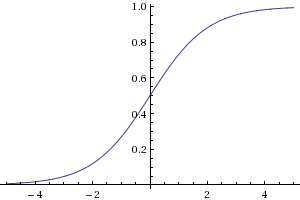
\includegraphics[width=0.6\textwidth]{logistic.png}
    \caption[Η λογιστική συνάρτηση]{Η λογιστική συνάρτηση}
 \end{figure}
 
 \paragraph{Ερμηνεία} Καθώς θέλουμε να κάνουμε μια πρόβλεψη για κάποιο άγνωστο χαρακτηριστικό με βάση κάποια άλλα χαρακτηριστικά-προβλέπτες που το αφορούν κινούμαστε στα εξής πλαίσια: αρχικά υπολογίζουμε πως επηρεάζει κάθε χαρακτηριστικό-προβλέπτης την άγνωστη ποσότητα, δηλαδή του δίνουμε κάποιο βάρος. Στη συνέχεια με βάση τα χαρακτηριστικά ενός δεδομένου παίρνουμε μία τιμή
για αυτό, την οποία θα μπορούσαμε να ερμηνεύσουμε ως το βαθμό που εμφανίζει το δεδομένο ως προς το χαρακτηριστικό που προβλέψουμε. Στη συνέχεια περνάμε αυτή τη τιμή  από ένα κατώφλι, ώστε να δούμε πού θα την κατατάξουμε. Η μαθηματική μετάφραση της παραπάνω διαδικασίας είναι η εξής:
$$s=w^T x \rightarrow h(x)=\theta(s)=\frac{e^{w^T x}}{1 + e^{w^T x} }$$
Η πραγματική πιθανότητα, που προσπαθούμε να προσεγγίσουμε  ορίζεται ως εξής:
$$P(y \mid x)=\left\{
	\begin{array}{ll}
		f(x)  & \mbox{if } y = +1 \\
		1 - f(x)  & \mbox{if } y = -1
	\end{array}
\right.$$

Αν υποθέσουμε πως η υπόθεσή μας είναι σωστή, δηλαδή $h=f$, τότε η πιθανότητα να πάρουμε έξοδο y για ένα δεδομένο με χαρακτηριστικά x είναι:
$$P(y \mid x)=\left\{
	\begin{array}{ll}
		h(x)  & \mbox{if } y = +1 \\
		1 - h(x)  & \mbox{if } y = -1
	\end{array}
\right.$$
 
Αν αντικαταστήσουμε με $h(x)=\theta(w^T x)$ και λαμβάνοντας υπόψιν πως $\theta(-s)= 1 - \theta(s)$, τότε η πιθανότητα  προκύπτει:
$$P(y \mid x)= \theta(y w^T x)$$
Ο παραπάνω τύπος λαμβάνει υπόψιν του μόνο ένα σημείο. Αν έχω N δεδομένα στο σετ εκπαίδευσης τότε η υπόθεσή μου γίνεται:
$$\prod_{n=1}^{N} P(y \mid x)= \prod_{n=1}^{N} \theta (y_n w^t x_n)$$
Η ερώτηση την οποία οφείλουμε να απαντήσουμε τώρα είναι : ”Δεδομένου του σετ εκπαίδευσης, ποιά είναι η πιθανότερη υπόθεση;” Η συνάρτηση, την οποία θέλουμε να ελαχιστοποιήσουμε, είναι η εξής:

$$Error(w)= \frac{1}{N} \sum_{n=1}^{N} \ln (1 + e^{- y_n w^T x_n} )$$

\paragraph{Gradient descent} Πρόκειται για έναν αλγόριθμο βελτιστοποίησης που προσπαθεί να βρει το τοπικό ελάχιστο μιας κυρτής συνάρτησης. Η διαδικασία είναι επαναληπτική και σε κάθε βήμα ο αλγόριθμος επιλέγει άπληστα να κινηθεί προς την πιο απότομη κατεύθυνση, που αντιστοιχεί στην αντίθετη κατεύθυνση της κλίσης στο συγκεκριμένο σημείο.
\begin{figure}[H]
	\centering			
    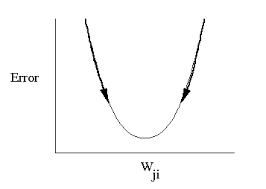
\includegraphics[width=0.6\textwidth, height=5cm]{gradient.png}
    \caption[Steepest descent]{Steepest descent}
 \end{figure}
 Εκτός από την κατεύθυνση προς την οποία θα κινηθεί ο αλγόριθμος πρέπει να επιλέξει και το μέγεθος του βήματος που θα εκτελέσει. Η παράμετρος αυτή επηρεάζει τόσο την ταχύτητα εκτέλεσης του αλγορίθμου, όσο και την επιτυχία του: αν τα βήματα που κάνει είναι σταθερά και μικρά, τότε θα φτάσει εγγυημένα σε κάποιο ελάχιστο, αλλά πολύ αργά, μειώνοντας την απόδοση του συστήματος. Αντιθέτως αν το βήμα είναι πολύ μεγάλο, μπορεί να υπερπηδά το ελάχιστο κάθε φορά που το πλησιάζει και ο αλγόριθμος να μην συγκλίνει ποτέ. Συνήθως υιοθετούμε μια πιο σύνθετη προσέγγιση: επιλέγουμε αρχικά μεγάλο βήμα, ώστε να πλησιάσουμε γρήγορα στη λύση και το μειώνουμε μόλις φτάσουμε κοντά.
 \begin{figure}[H]
    \centering
    \begin{minipage}{.5\textwidth}
        \centering
        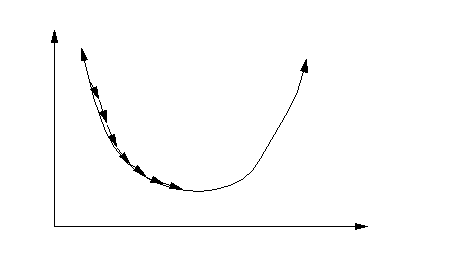
\includegraphics[width=0.8\linewidth, height=0.15\textheight]{smallstep.png}
        \caption[Gradient descent με πολύ μικρό βήμα]{Gradient descent με πολύ μικρό βήμα}
        
    \end{minipage}%
    \begin{minipage}{0.5\textwidth}
        \centering
        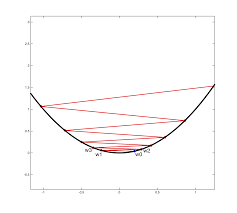
\includegraphics[width=0.8\linewidth, height=0.15\textheight]{bigstep.png}
        \caption[Gradient descent με πολύ μεγάλο βήμα]{Gradient descent με πολύ μεγάλο βήμα}
       
    \end{minipage}
\end{figure}
\subsubsection{Μηχανές διανυσματικής στήριξης}
Πρόκειται για μία από τις πιο πρόσφατες τεχνικές στον τομέα της επιβλεπόμενης μάθησης, που χρησιμοποιείται ευρέως τόσο σε προβλήματα ταξινόμησης, όσο και σε προβλήματα παλινδρόμησης.
Έστω ότι βρισκόμαστε μπροστά από ένα πρόβλημα ταξινόμησης, με την κλάση να παίρνει 2 τιμές και τα παραδείγματα να έχουν 2 χαρακτηριστικά. Τότε ο χώρος μας είναι κάπως έτσι:
\begin{figure}[H]
	\centering			
    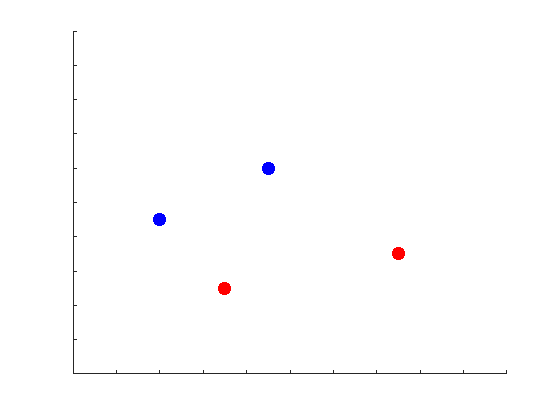
\includegraphics[width=0.6\textwidth, height=6cm]{svm_dots.png}
    \caption[Χώρος ταξινόμησης μηχανής διανυσματικής στήριξης]{Χώρος ταξινόμησης}
 \end{figure}
 Θα θέλαμε η υπόθεσή μας να διαχωρίσει τα παραπάνω δεδομένα με βάση την κλάση τους, πράγμα που διαπιστώνουμε πως μπορεί να επιτευχθεί με μερικές διαφορετικές υποθέσεις:
  \begin{figure}[H]
    \centering
    \begin{minipage}{.333\textwidth}
        \centering
        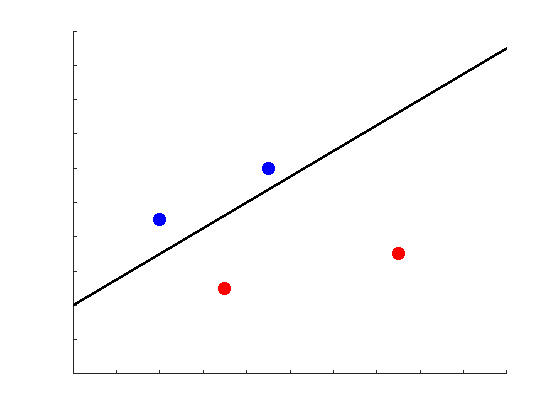
\includegraphics[width=\linewidth, height=0.15\textheight]{svm_line1.png}
        \caption[Υπόθεση Α μηχανής διανυσματικής στήριξης]{Υπόθεση Α}
        
    \end{minipage}%
    \begin{minipage}{0.333\textwidth}
        \centering
        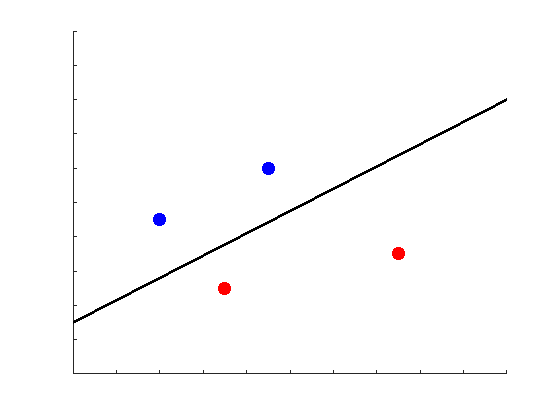
\includegraphics[width=\linewidth, height=0.15\textheight]{svm_line2.png}
        \caption[Υπόθεση Β μηχανής διανυσματικής στήριξης]{Υπόθεση Β}
       
    \end{minipage}
     \begin{minipage}{0.333\textwidth}
        \centering
        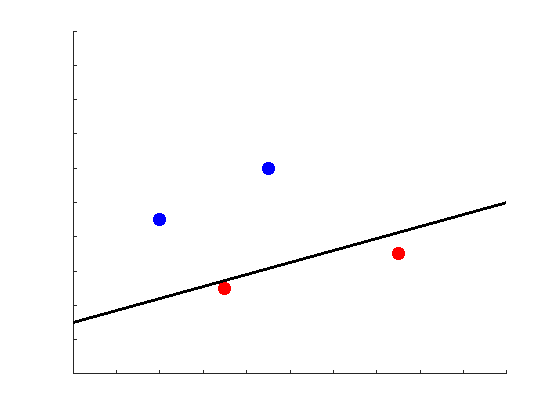
\includegraphics[width=\linewidth, height=0.15\textheight]{svm_line3.png}
        \caption[Υπόθεση Γ μηχανής διανυσματικής στήριξης]{Υπόθεση Γ}
       
    \end{minipage}
\end{figure}
Οι μηχανές διανυσματικής στήριξης μπορούν να απαντήσουν στο εύλογο ερώτημα: ”Ποια από τις παραπάνω υποθέσεις είναι η καλύτερη;” Λαμβάνοντας υπόψιν πως η ποιότητα μιας υπόθεσης καθορίζεται βασικά από την ικανότητά της να γενικεύει, οι αλγόριθμοι αυτοί επιλέγουν την υπόθεση έτσι, ώστε τα πιο κοντινά σημεία που ταξινομούνται σε διαφορετικές κατηγορίες να χωρίζονται από όσο το δυνατόν
μεγαλύτερο κενό. Τα σημεία αυτά ονομάζονται διανύσματα στήριξης. Ένας πιο επίσημος ορισμός, που επεκτείνεται σε περισσότερες διαστάσεις, είναι πως ορίζεται ένα υπερεπίπεδο που διαχωρίζει τις κατηγορίες.

\paragraph{Θεωρητική θεμελίωση} Έστω πως τα δεδομένα μας είναι δισδιάστατα και επιχειρούμε να ορίσουμε την ευθεία που εξασφαλίζει μεγαλύτερο κενό μεταξύ των κοντινότερων σημείων που ανήκουν σε διαφορετική κλάση. Η ευθεία που αναζητούμε φαίνεται στο παρακάτω σχήμα και δίνεται από τον τύπο $w^T x = 0$ και οι ευθείες που περνούν από τα διανύσματα στήριξης ορίζονται ως $w^T x = 1$ και$ w^T x =-1$
\begin{figure}[H]
	\centering			
    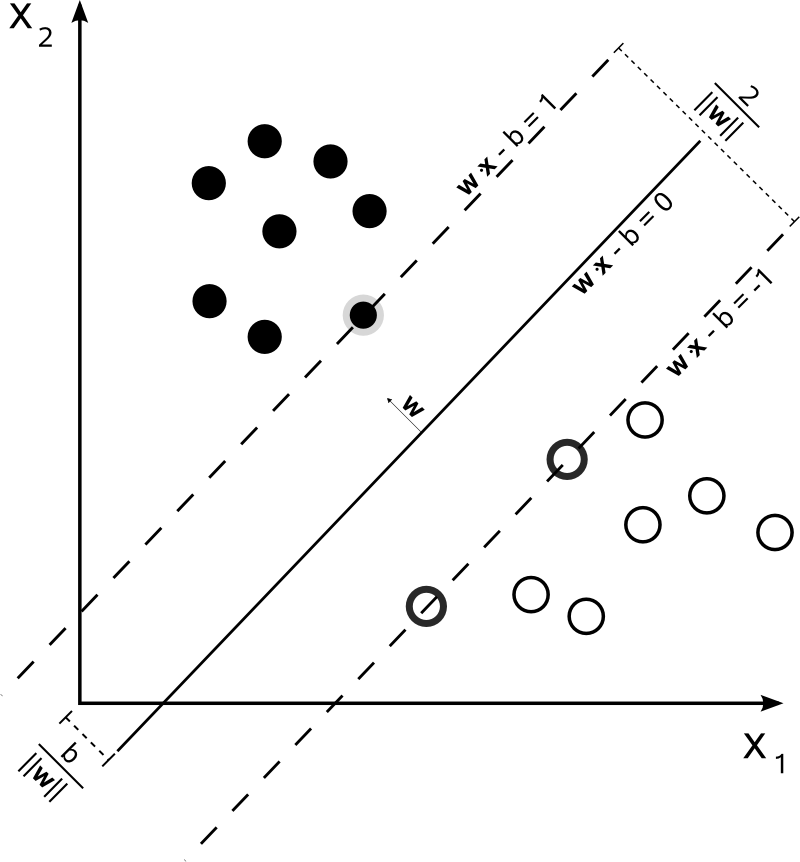
\includegraphics[scale=0.2]{svm.png}
    \caption[Υπερεπίπεδο μηχανών διανυσματικής στήριξης]{Υπερεπίπεδο μηχανών διανυσματικής στήριξης}
 \end{figure}
 Πριν συνεχίσουμε θα χρειαστεί να ορίσουμε δύο τεχνικές παραδοχές:
 \begin{itemize}
 \item Όπως είναι γνωστό, ένα επίπεδο είναι αμετάβλητο ως προς την κλιμάκωση, δηλαδή με όποια σταθερά και να το πολλαπλασιάσω θα συνεχίσω να έχω το ίδιο επίπεδο. Για αυτό θα κανονικοποιούμε ώστε $\norm{w^T x}=1$
 \item  Μας βολεύει να βγάλουμε τον σταθερό όρο $w_0$ από το διάνυσμα w και να ορίσουμε την επιφάνεια ως $w^T  x + b = 0$, όπου προφανώς το b αντιστοιχεί στο $w_0$.

 \end{itemize}
 
 Πώς υπολογίζουμε την απόσταση ενός σημείου από ένα υπερεπίπεδο;
Αρχικά παρατηρώ πως το w είναι κάθετο στο υπερεπίδεδο. Αυτό αποδεικνύεται πολύ εύκολα ως εξής: Έστω δύο σημεία $x^,$ και $x^{,,}$ πάνω στο υπερεπίπεδο. Τότε ισχύει $w^T  x^, + b = 0$ και $w^T  x^{,,} + b = 0$. Επομένως $w^T (x^, -  x^{,,}) = 0$, δηλαδή το w είναι κάθετο σε οποιαδήποτε ευθεία ενώνει δύο σημεία του υπερεπιπέδου.

 Η απόσταση του σημείου $x_n$ από το υπερεπίπεδο υπολογίζεται ως εξής: παίρνω οποιοδήποτε σημείο x στο υπερεπίπεδο και προβάλλω το διάνυσμα $x_n - x$ στο w. Η πράξη αυτή, με το κανονικοποιημένο w να ορίζεται ως $\bar{w}=\frac{w}{\norm{w}}$ , δίνεται από τον τύπο:
$$
distance=\abs{\bar{w} (x_n -x)} =\frac{1}{\norm{w}} \abs{w^T x_n - w^T x}
=\frac{1}{\norm{w}} \abs{w^T x_n  +b - w^T x -b}=\frac{1}{\norm{w}} \\
$$ 
Η προσθαφαίρεση του b μας βοήθησε να παρατηρήσουμε πως το πρώτο άθροισμα ισούται με 1, λόγω της πρώτης παραδοχής, και το δεύτερο άθροισμα δίνει 0, καθώς αποτελεί την εξίσωση του υπερεπιπέδου.

Στη συνέχεια θα προσπαθήσουμε να ορίσουμε το πρόβλημα που προσπαθούν να επιλύσουν οι μηχανές διανυσματικής στήριξης και να το φέρουμε σε τέτοια μορφή, ώστε η επίλυσή του να είναι εύκολη και αυτοματοποιημένη.

 Tο πρόβλημα που θέλουμε να βελτιστοποιήσουμε είναι το εξής: θέλουμε να μεγιστοποιήσουμε την απόσταση ενός οποιουδήποτε σημείου από το υπερεπίπεδο υπό τον περιορισμό ότι για το κοντινότερο σημείο, έχουμε κανονικοποιήσει ώστε να ισχύει η εξίσωση $w^T x_n = 1$. Η μαθηματική διατύπωση αυτού του προβλήματος είναι η εξής:
 \begin{flalign*}
\text{Μεγιστοποίηση} && \frac{1}{\norm{w}} &&\\
\text{υπό τον περιορισμό ότι} && \min_{n=1,2,...,N} \abs{w^T x + b}=1
\end{flalign*}
Η παραπάνω διατύπωση δεν είναι φιλική προς επίλυση, κυρίως λόγω της μορφής του περιορισμού, για αυτό θα την αναδιατυπώσουμε ως εξής:
 \begin{flalign*}
\text{Ελαχιστοποίηση} && \frac{1}{2} w^T w &&\\
\text{υπό τον περιορισμό ότι} && y_n(w^T x_n + b) \geq 1, n=1,...,N
\end{flalign*} 
\\
\fbox{\begin{minipage}{\textwidth}
\begin{center}
Πολλαπλασιαστές Lagrange
\end{center} 
Πρόκειται για μία μέθοδο εύρεσης τοπικών μεγίστων ή ελαχίστων μιας συνάρτησης που υπακούει σε κάποιον περιορισμό ισότητας. Αν ο σκοπός μου είναι να μεγιστοποιήσω μια συνάρτηση $f(x,y)$ υπό τον περιορισμό ότι $g(x, y) = 0$, τότε αυτή η μέθοδος ορίζει και επιλύει τη συνάρτηση Lagrange $L(x, y, \lambda) = f(x,y) - \lambda g(x,y) $, εισάγοντας μια θετική μεταβλητή χαλαρότητας $\lambda$. Οι προϋποθέσεις Karush–Kuhn–Tucker, επεκτείνουν την εφαρμογή των πολλαπλασιαστών Lagrange,  επιτρέποντας τη βελτιστοποίηση προβλήματα υπό περιορισμούς σε μορφή ανισοτήτων.
\end{minipage}}
Η εξίσωση Lagrange, που προκύπτει από το παραπάνω πρόβλημα με τη βοήθεια των προϋποθέσεων Karush–Kuhn–Tucker, είναι η εξής:
 \begin{flalign*}
\text{Ελαχιστοποίηση} &&L(w,b,a)&= \frac{1}{2} w^T w - \sum_{n=1}^{N} a_n (y_n(w^T x_n +b) -1) &&
\end{flalign*}

όπου a είναι η θετική μεταβλητή χαλαρότητας που εισήγαγαν οι πολλαπλασιαστές Lagrange.
Για να ελαχιστοποιήσω ως προς τα w και b, αρκεί να βρω τις μερικές παραγώγους και να τις μηδενίσω:
 \begin{flalign*}
\text{Άρα} && \nabla_w L &= w-\sum_{n=1}^{N} a_n y_n x_n=0  &&\\
\text{και} && \frac{\partial L}{\partial b}&= \sum_{n=1}^{N} a_n y_n =0 &&
\end{flalign*}

Αντικαθιστώντας στην αρχική εξίσωση, το πρόβλημα βελτιστοποίησης διατυπώνεται ως εξής:
\begin{flalign*}
\text{Ελαχιστοποίηση} && L(a)= \sum_{n=1}^{N} a_n - \frac{1}{2} \sum_{n=1}^{N} \sum_{m=1}^{N} y_n y_m a_n a_m x_n^T x_m  &&\\
\text{υπό τη συνθήκη} && \sum_{n=1}^{N} a_n y_n =0 &&\\
\text{και} && a_n \geq 0  &&
\end{flalign*}
\fbox{\begin{minipage}{\textwidth}
\begin{center}
Τετραγωνικός Προγραμματισμός
\end{center} 
Είναι μια ειδική υποκατηγορία μαθηματικής βελτιστοποίησης, που ασχολείται με τη
βελτιστοποίηση τετραγωνικών συναρτήσεων μεταβλητών που υπόκεινται σε γραμμικούς περιορισμούς. Στόχος του είναι να βρουν το n-διάστατο διάνυσμα x που ελαχιστοποιεί τη συνάρτηση $\frac{1}{2} x^T Q x + c^T x$ υπό τον περιορισμό $x \leq b$
\end{minipage}}

Η λύση του παραπάνω προβλήματος δίνεται από κάποιο πακέτο τετραγωνικού περιορισμού, όπου το Q διατυπώνεται ως εξής:
 \[
\begin{bmatrix}
    y_1y_1x_1^Tx_1 & y_1y_2x_1^Tx_2   & \dots  &  y_1y_Nx_1^Tx_N \\
     y_2y_1x_2^Tx_1 & y_2y_2x_2^Tx_2   & \dots  &  y_2y_Nx_2^Tx_N \\
    \vdots  & \vdots &\ddots & \vdots \\
     y_Ny_1x_N^Tx_ 1& y_Ny_2x_N^Tx_2   & \dots  &  y_Ny_Nx_N^Tx_N \\
\end{bmatrix}
\]

Καταφέραμε να διατυπώσουμε το πρόβλημα που επιλύουν οι μηχανές διανυσματικής στήριξης σε όρους προβλήματος βελτιστοποίησης που επιλύεται σχετικά εύκολα. Πρόβλημα θα συναντήσουμε όταν το πλήθος των παρατηρήσεων Ν είναι τόσο μεγάλο ώστε να δίνει στον πίνακα Q απαγορευτικό μέγεθος.

 
 \paragraph{Μη γραμμικά διαχωρίσιμες κλάσεις}
 Μέχρι τώρα είδαμε πως οι αλγόριθμοι αυτοί σχηματίζουν υπερεπίπεδα, επομένω κάποιος θα μπορούσε να συμπεράνει πως λειτουργούν μόνο για γραμμικά διαχωρίσιμα προβλήματα. Ωστόσο, αν καταφέρω να μετασχηματίσω τα δεδομένα μου σε κάποιο χώρο μεγαλύτερων διαστάσεων, όπου είναι γραμμικά διαχωρίσιμα, και βρω τα διανύσματα στήριξης εκεί, τότε μπορώ με τον αντίστροφο μετασχηματισμό να βρω τα διανύσματα στήριξης στον αρχικό μου χώρο.
 \begin{figure}[H]
	\centering			
    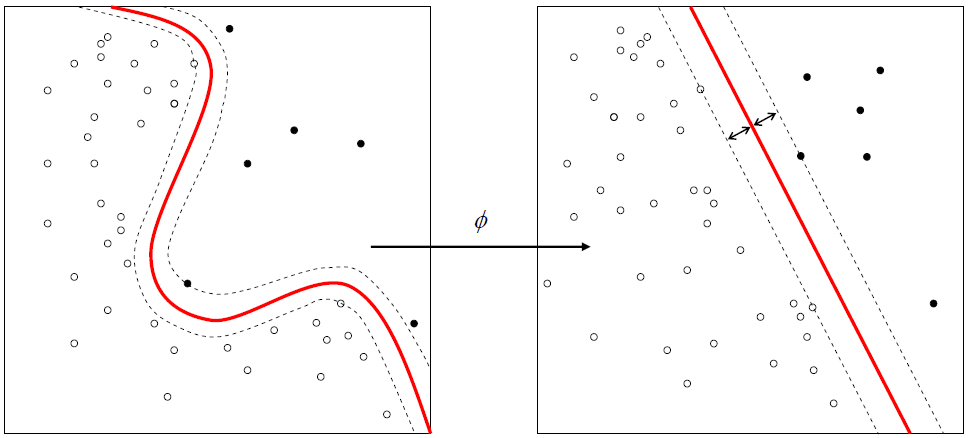
\includegraphics[width=0.8\textwidth, height=6cm]{kernel.png}
    \caption[Χρήση πυρήνα για επίλυση μη γραμμικού διαχωρισμού]{Χρήση πυρήνα για επίλυση μη γραμμικού διαχωρισμού}
 \end{figure}
 
 Έστω πως εκτελώ τον εξής μετασχηματισμό:
 $$X \rightarrow Z$$
 Αν παρατηρήσω την τελική διατύπωση του προβλήματος που επιλύουν αυτοί οι αλγόριθμοι, θα δω πως η μόνη επίδραση αυτού του μετασχηματισμού είναι πως στη θέση των εσωτερικών γινομένων μεταξύ των x, πλέον πρέπει να υπολογίζω εσωτερικά γινόμενα μεταξύ των z σημείων.
 
Η παραπάνω διαπίστωση μπορεί με μια πρώτη ματιά να μην προκαλεί ενδιαφέρον, αποτέλεσε ωστόσο τον ακρογωνιαίο λίθο στον οποίο βασίζεται η ανωτερότητα αυτής της οικογένειας αλγορίθμων. Ας θεωρήσουμε ένα πρόβλημα ταξινόμησης, όπου τα δεδομένα είναι τόσο περίπλοκα, που προκειμένου να γίνει ο γραμμικός διαχωρισμός τους, να απαιτείται η μεταφορά τους σε κάποιο χώρο τεραστίων, δυνητικά άπειρων διαστάσεων. Εκεί που οι περισσότεροι αλγόριθμοι σηκώνουν τα χέρια ψηλά, οι μηχανές διανυσματικές στήριξης κάνουν την εξής σχεδιαστική επιλογή: αντί να μεταφέρουν τα χαρακτηριστικά σε έναν άπειρο χώρο και να επιλύσουν εκεί το πρόβλημα, ορίζουν μόνο αυτό που χρειάζονται, δηλαδή το εσωτερικό γινόμενο μεταξύ διανυσμάτων στον καινούριο χώρο. Το γινόμενο αυτό αποτελεί μία συνάρτηση που ονομάζεται πυρήνας και συμβολίζεται ως εξής: 
$$K(x, x^,)= z \cdot z^,$$
Σε αυτό το σημείο, μπορεί να αναρωτηθεί κάποιος πώς μπορεί να ορίσει έναν πυρήνα, χωρίς να έχει αντίληψη του χώρου, στον οποίο θα μεταφερθεί. Η λογική είναι κάπως ανάποδη: αρκεί να ορίσω μια κάποια συνάρτηση και στη συνέχεια να μπορώ να αποδείξω ότι μπορεί να προκύψει ως εσωτερικό γινόμενο δύο μετασχηματισμένων διανυσμάτων. Υπάρχει μάλιστα η συνθήκη του Mercer, που εξασφαλίζει πως οποιαδήποτε συνάρτηση πυρήνα
$$K(x, x^,)$$
είναι έγκυρη, αρκεί να είναι συμμετρική και ο πίνακας που ακολουθεί να είναι θετικά ημιορισμένος:
 \[
\begin{bmatrix}
    (x_1, x_1) &  (x_1, x_2)  & \dots  &   (x_1, x_N) \\
     (x_2, x_1) &  (x_2 x_2)  & \dots  &   (x_2, x_N) \\
    \vdots  & \vdots &\ddots & \vdots \\
    (x_N, x_1) &  (x_N, x_2)  & \dots  &   (x_N, x_N) \\
\end{bmatrix}
\]
Κατά κανόνα η επιλογή του πυρήνα γίνεται από μια λίστα συχνά χρησιμοποιούμενων συναρτήσεων:
\begin{itemize}
\item \textit{Πολυωνυμικός.} Δίνεται από τον τύπο:
$$K(x, x^,)= (x^T x^, + c)^d$$
όπου d είναι η διάσταση του νέου χώρου και c μία παράμετρος που καθορίζει την επιρροή που έχουν οι όροι μεγαλύτερης τάξης σε σχέση με τους όρους μικρότερης τάξης.
\item \textit{Γκαουσιανός (Radial basia function).} Δίνεται από τον τύπο:
$$K(x, x^,)= e^{(-\frac{\norm{x-x^,}^2}{2 \sigma ^2})}$$
Ο πυρήνας αυτός μας μεταφέρει σε ένα χώρο άπειρων διαστάσεων. Ο αριθμητής του εκθέτη υπολογίζει την ευκλείδεια απόσταση μεταξύ των 2 σημείων, οπότε μπορούμε να τον αντιληφθούμε ως ένα μέτρο ομοιότητας.
\end{itemize}
\paragraph{Μηχανές διανυσματικής στήριξης χαλαρού περιθωρίου}Κάθε φορά λοιπόν που παρατηρούμε μη γραμμικότητα στα δεδομένα μας θα εφαρμόζουμε τη συνάρτηση
πυρήνα; Ας δούμε το παρακάτω παράδειγμα:
 \begin{figure}[H]
    \centering
    \begin{minipage}{.5\textwidth}
        \centering
        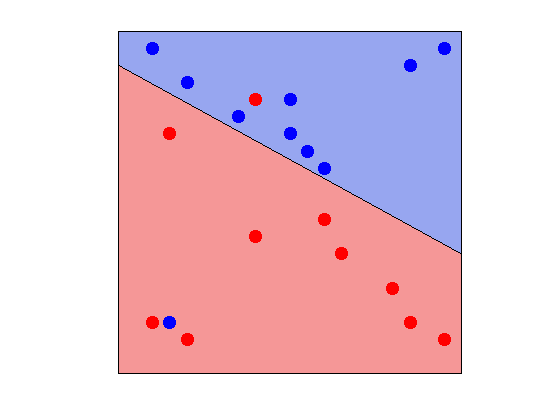
\includegraphics[width=\linewidth, height=0.15\textheight]{soft1.png}
        \caption[Ελάχιστα μη διαχωρίσιμα δεδομένα]{Ελάχιστα μη διαχωρίσιμα δεδομένα}
        
    \end{minipage}%
    \begin{minipage}{0.5\textwidth}
        \centering
        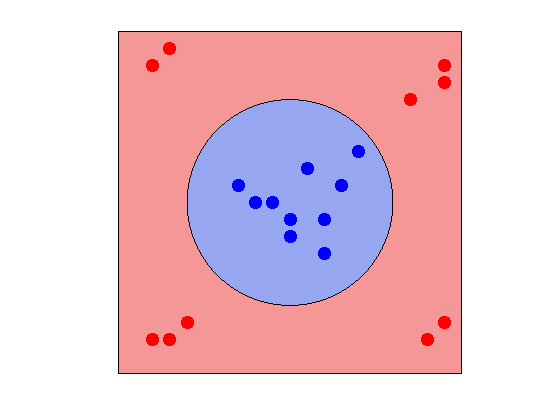
\includegraphics[width=\linewidth, height=0.15\textheight]{soft2.png}
        \caption[Εμφανώς μη διαχωρίσιμα δεδομένα]{Εμφανώς μη διαχωρίσιμα δεδομένα}
       
    \end{minipage}
    \end{figure}
Και τα δύο σχήματα αντιστοιχούν σε μη γραμμικά διαχωρίσιμα προβλήματα, ωστόσο
διαφοροποιούνται ποιοτικά: στα αριστερά, ένας γραμμικός διαχωρισμός θα προκαλούσε πολύ μικρό σφάλμα, καθώς μόνο δύο παραδείγματα του σετ εκπαίδευσης θα κατηγοριοποιηθούν λανθασμένα. Αν προσπαθήσω να τα κατατάξω και αυτά σωστά, τότε η υπόθεσή μου θα γίνει πολύ περίπλοκη, καθώς θα χρειαστούν πολλά διανύσματα στήριξης και υποπτεύομαι πως το μοντέλο μου δεν θα γενικεύει. Αντιθέτως, η δεξιά εικόνα αντιστοιχεί σε εμφανώς μη γραμμικά διαχωρίσιμο πρόβλημα, που επιλύεται μόνο με τη χρήση συνάρτησης πυρήνα.

Η απαίτηση δυνατότητας λανθασμένης κατηγοριοποίησης υλοποιείται με μια ειδική κατηγορία των μηχανών διανυσματικής στήριξης: τις μηχανές χαλαρού περιθωρίου. Στους αλγόριθμους αυτούς το υπερεπίπεδο ορίζεται κανονικά, ώστε να μεγιστοποιείται το χάσμα, ωστόσο επιτρέπεται σε κάποια σημεία να το παραβιάσουν, δηλαδή να βρεθούν πέρα από τη νοητή γραμμή του περιθωρίου που ορίζεται από τα διανύσματα στήριξης της κατηγορίας τους.

 \begin{figure}[H]
	\centering			
    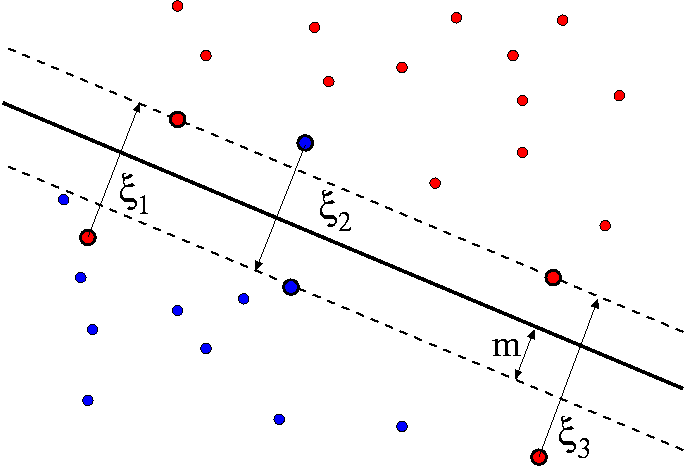
\includegraphics[width=0.8\textwidth, height=6cm]{violation.png}
    \caption[Μηχανές διανυσματικής στήριξης χαλαρού περιθωρίου]{Μηχανές διανυσματικής στήριξης χαλαρού περιθωρίου}
 \end{figure}
 
 Μαθηματικά, οι αλγόριθμοι αυτοί διατυπώνονται ως εξής: Η εξίσωση που ορίζει το περιθώριο εκατέρωθεν του υπερεπιπέδου διαχωρισμού $y_n (w^T x_n + b) \geq 1, n=1,..., N$ πλέον παραβιάζεται, οπότε εισάγουμε μια μεταβλητή χαλαρότητας, την $\xi_n$, ώστε :
 $$y_n (w^T x_n + b) \geq 1 - \xi_n, n=1, ..., N$$
 και η εξίσωση που βελτιστοποιεί πλέον ο αλγόριθμος είναι:
  \begin{flalign*}
\text{Ελαχιστοποίηση} && \frac{1}{2} w^T w + C \sum_{n=1}^{N} \xi_n  &&\\
\text{υπό τον περιορισμό ότι} &&y_n (w^T x_n + b) \geq 1 - \xi_n, n=1, ..., N  &&\\
\text{και} && \xi_n \geq 0  &&
\end{flalign*}
Ο παράγοντας C προσδιορίζει πόσο αυστηρός είναι ο αλγόριθμος ως προς τη παραβίαση του περιθωρίου: μία μεγάλη τιμή του C δηλώνει πως επιθυμώ πολύ μικρή παραβίαση.
\subsection{Τεχνικές αξιολόγησης μοντέλων}
Είδαμε πως τόσο κατά τη ρύθμιση του μοντέλου στη διάρκεια της εκπαίδευσης, όσο και για την τελική αξιολόγηση του μοντέλου για τη διαπίστωση της ικανότητάς του να γενικεύει χρειαζόμαστε δύο ανεξάρτητα σετ: ένα, στο οποίο θα γίνεται η εκπαίδευση και ένα στο οποίο θα γίνεται η αξιολόγηση του μοντέλου. Φυσικά τα δεδομένα μας δίνονται ενιαία και ο τρόπος με τον οποίο θα διαχωριστούν αποτελεί σχεδιαστική επιλογή. Όπως έχει συνηθίσει, ο ειδικός οφείλει να συμβιβαστεί μεταξύ δύο σκοπών: τη
χρήση όσο το δυνατόν μεγαλύτερου σετ εκπαίδευσης, για να παραχθεί ένα πιο ”σοφό” μοντέλο, αλλά και σετ ελέγχου, ώστε η γενίκευση να είναι εγγυημένη, λαμβάνοντας υπόψιν το πεπερασμένο του σετ δεδομένων και του διαθέσιμου χρόνου.
\paragraph{Hold out} Η τεχνική αυτή είναι πολύ απλή: αναθέτουμε ένα μέρος των δεδομένων για εκπαίδευση και τα υπόλοιπα τα αφήνουμε στην άκρη για αξιολόγηση. Οι συνήθεις αναλογίες είναι $80\%-20\%$ και $75\%-25\%$ εκπαίδευση και αξιολόγηση αντίστοιχα. Αν και γρήγορη, η τεχνική αυτή δεν προτιμάται, καθώς δεν εγγυάται την αξιοπιστία του αποτελέσματος και συρρικνώνει πολύ το σετ εκπαίδευσης.
\paragraph{Leave one out} Με την τεχνική αυτή μεγιστοποιούμε το μέγεθος των δύο σετ εις βάρος του χρόνου της μάθησης: κάθε φορά εκπαιδεύουμε το μοντέλο με όλα τα δεδομένα εκτός από ένα και το αξιολογούμε σε αυτό και επαναλαμβάνουμε τη διαδικασία όσες φορές είναι τα δεδομένα μας αφήνοντας κάθε φορά ένα διαφορετικό για αξιολόγηση.
\paragraph{Cross-validation}Αυτή είναι η συνηθέστερη τεχνική, καθώς εξασφαλίζει μικρούς χρόνους μάθησης και αξιόπιστο αποτέλεσμα τόσο από πλευρά εκπαίδευσης όσο και από πλευρά αξιολόγησης. Τα δεδομένα χωρίζονται σε k υποσύνολα, το μοντέλο εκπαιδεύτει με τα $k-1$ και αξιολογείται με το εναπομείναν. Η διαδικασία επαναλαμβάνεται k φορές, ώστε όλα τα υποσύνολα να χρησιμοποιηθούν μια φορά για
αξιολόγηση. Τελικά η απόδοση του μοντέλου υπολογίζεται ως ο μέσος όρων των επιδόσεων στα k υποσύνολα. Συνήθως το k επιλέγεται ως $10$, οπότε μιλάμε για $10$-fold cross-validation. 
\paragraph{.632 bootstrap} Η τεχνική αυτή προσπαθεί να πετύχει το στόχο του cross validation, με διαφορετική όμως λογική: αντί να τεμαχίζουμε το σετ εκπαίδευσης, δημιουργούμε k αντίγραφά του με τυχαία δειγματοληψία με αντικατάσταση, το καθένα από τα οποία αποτελείται από Ν στοιχεία. Αν λοιπόν το αρχικό σετ δεδομένων ήταν:
 \[
S=
\begin{bmatrix}
    y_1 &  x_{11}  & \dots  &   x_{1p} \\
    \vdots  & \vdots &\ddots & \vdots \\
    y_N &  x_{N1}  & \dots  &   x_{Np} \\
\end{bmatrix}
\]
τότε κάθε δείγμα ορίζεται ως:
 \[
S_b=
\begin{bmatrix}
    y_1^{*b} &  x_{11}^{*b}  & \dots  &   x_{1p}^{*b} \\
    \vdots  & \vdots &\ddots & \vdots \\
    y_N^{*b} &  x_{N1}^{*b}  & \dots  &   x_{Np}^{*b} \\
\end{bmatrix}
\]
Στη συνέχεια μπορούμε να εκπαιδεύσουμε ένα διαφορετικό μοντέλο $\bar{f}^{*b}(x)$ με κάθε δείγμα και να υπολογίσουμε το σφάλμα ως εξής:
$$\bar{E_{boot}}=\frac{1}{B} \frac{1}{N} \sum_{b=1}^{B} \sum_{i=1}^{N} L(y_i,\bar{f}^{*b}(x))$$
Ο παραπάνω δείκτης είναι πολωμένος, καθώς υπάρχει η πιθανότητα δεδομένα που έχουν χρησιμοποιηθεί για την εκπαίδευση ενός μοντέλου να χρησιμοποιηθούν και για την αξιολόγησή του. Η πιθανότητα αυτή, όπως προκύπτει λόγω της τυχαίας δειγματοληψίας με αντικατάσταση είναι πολύ μεγάλη:
$$P[(y_i, x_i) \in S_b]= 1- (1- \frac{1}{N})^N \approx 1- e^{-1} \approx 0.632$$
Την παθογένεια αυτή επιχειρεί να λύσει η τεχνική του leave-one-out bootstrap cross-validation, όπου τα στοιχεία δε χρησιμοποιούνται για την αξιολόγηση ενός μοντέλου, στην εκπαίδευση του οποίου έχουν συμμετάσχει:
$$\bar{E}^{(1)}= \frac{1}{N} \sum_{i=1}^{N} \frac{1}{\abs{C^{-i}}} \sum_{b \in C^{-i}} L(y_i, \bar{f}^{*b}(x_i) )$$

όπου $C^{-i}$ είναι τα δείγματα που δεν περιέχουν το στοιχείο i και $\abs{C^{-i}}$ είναι το πλήθος στοιχείων του αντίστοιχου δείγματος.
Η παραπάνω μετρική συνεχίζει ωστόσο να είναι πολωμένη λόγω της συχνής επαναχρησιμοποίησης δεδομένων: κάθε δείγμα  περιέχει κατά μέσο όρο $0.632 \cdot N$ διαφορετικά στοιχεία, χαρακτηριστικό που θυμίζει 2-fold cross-validation.

Έτσι, προτάθηκε η συμβιβαστική λύση του .632 bootstrap():
$$\bar{E}^{(0.632)}= 0.368 \cdot \bar{err} + 0.632 \cdot \bar{E}^{(1)} $$
όπου $\bar{err}$ είναι το σφάλμα που υπολογίζεται για τα σημεία που έχουν συμμετάσχει στην εκπαίδευση.

Αυτή η μετρική προσπαθεί να σταθμίσει τη συνεισφορά δύο αντίθετα πολωμένων όρων. Ο πρώτος αποτελεί τον απλό εκτιμητή και λειτουργεί σωστά για σημεία που δεν απέχουν καθόλου από το σετ εκπαίδευσης. Ο δεύτερος έχει υποθέσει τη μεγαλύτερη απόσταση των νέων δεδομένων από το σετ εκπαίδευσης (η πιθανότητα ένα στοιχείο να μη συμμετέχει σε ένα δείγμα είναι $0.368$).

\subsection{Τεχνικές επιλογής χαρακτηριστικών}
\subsubsection{Ανάλυση κυρίαρχων συνιστωσών}
Η τεχνική αυτή προέρχεται από τη γραμμική άλγεβρα και εφαρμόζεται με στόχο την εξαγωγή χρήσιμων χαρακτηριστικών σε προβλήματα μηχανικής μάθησης. Το όνομά της προδίδει τη λειτουργία της: την εύρεση των κυρίαρχων συνιστωσών στα δεδομένα.

Τα δεδομένα σε ένα πρόβλημα ταξινόμησης αποτελούνται από τα χαρακτηριστικά και την κλάση πρόβλεψης. Γεωμετρικά, μπορούμε να αντιληφθούμε τα χαρακτηριστικά ως διανύσματα-βάσεις και τις τιμές κάθε παραδείγματος ως τις προβολές σε αυτή τη βάση. Σκοπός της ανάλυσης κυρίαρχων συνιστωσών είναι να βρει μια νέα βάση για τα δεδομένα, στην οποία αυτά θα περιγράφονται ‘’καλύτερα’’. Αν λοιπόν τα αρχικά μας δεδομένα βρίσκονται στον πίνακα Χ, τότε αρκεί να βρούμε έναν πίνακα μετασχηματισμού P που θα μας μεταφέρει στη νέα βάση, δηλαδή:
$$Y=P X$$
Προκειμένου να ορίσουμε τον πίνακα P, οφείλουμε να αναλογιστούμε το σκοπό των ενεργειών μας: Τί είναι αυτό που μας ενοχλεί στην αρχική βάση και πώς ορίζουμε την καλύτερη έκφραση των δεδομένων; Σε αυτό το σημείο θυμόμαστε δύο παθογένειες των δεδομένων: το θόρυβο και τη περίσσεια πληροφορίας. Και τα δύο αυτά προβλήματα σχετίζονται άμεσα με την έννοια της αυτοσυσχέτισης: ο μεν θόρυβος είναι εξ ορισμού ασυσχέτιστος με όλα τα χαρακτηριστικά, η δε περίσσεια πληροφορίας ποσοτικοποιείται μέσω της αυτοσυσχέτισης μεταξύ των χαρακτηριστικών. Ο πίνακας αυτοσυσχέτισης των αρχικών δεδομένων ορίζεται ως:
$$S_X=\frac{1}{n-1} X X^T$$
Προκύπτει λοιπόν μία αναγκαιότητα για τα μετασχηματισμένα δεδομένα Y: ο πίνακας αυτοσυσχέτισής τους οφείλει να είναι διαγώνιος, δηλαδή κάθε χαρακτηριστικό να συσχετίζεται μόνο με τον εαυτό του. Ο πίνακας που επιθυμούμε να διαγωνοποιήσουμε είναι λοιπόν:
\begin{equation*} 
\begin{split}
S_Y & = \frac{1}{n-1} Y Y^T \\
 & = \frac{1}{n-1} (PX)(PX)^T \\
  & = \frac{1}{n-1} PXX^TP^T\\
   & = \frac{1}{n-1} P(XX^T)P^T\\
    & = \frac{1}{n-1} PAP^T
\end{split}
\end{equation*}
όπου $A=XX^T$.

Σύμφωνα με τη θεωρία της γραμμικής άλγεβρας, ένας πίνακας Α διαγωνοποιείται  με τη βοήθεια ενός πίνακα, κάθε στήλη του οποίου είναι ένα ιδιοδιάνυσμα του Α, δηλαδή:
$$A=EDE^T$$
όπου ο D είναι ένας διαγώνιος πίνακς και Ε ένας πίνακας με στήλες τα ιδιοδιανύσματα του Α. 

Αν λοιπόν επιλέξουμε τον πίνακα P, έτσι ώστε κάθε γραμμή του να είναι ιδιοδιάνυσμα του A, τότε πετυχαίνουμε:
\begin{equation*} 
\begin{split}
S_Y & = \frac{1}{n-1} PAP^T \\
 & = \frac{1}{n-1} P(P^TDP)P^T \\
  & = \frac{1}{n-1} (PP^T)D(PP^T)\\
   & = \frac{1}{n-1}(PP^{-1})D(PP^{-1})\\
    & = \frac{1}{n-1} D
\end{split}
\end{equation*} 
δηλαδή ο πίνακας Υ έχει διαγώνιο πίνακα ετεροσυσχέτισης και μπορούμε να πούμε πως τα κυρίαρχα συστατικά είναι οι γραμμές του P, δηλαδή τα ιδιοδιανύσματα του X και οι διαγώνιες τιμές του πίνακα $S_Y$ είναι η διακύμανση κατά μήκος των κυρίαρχων συστατικών.

Συνήθως κατά την εξαγωγή χαρακτηριστικών προσπαθούμε να απλοποιήσουμε την περιγραφή των δεδομένων διατηρώντας όσο το δυνατόν περισσότερη πληροφορία. Έτσι, μετά την εφαρμογή της ανάλυσης κυρίαρχων συνιστωσών μπορούμε να επιλέξουμε να κρατήσουμε τα διανύσματα που μας δίνουν ένα ικανοποιητικό μέρος της διακύμανσης, συνήθως το $ 97\% -98\% $. Σε εφαρμογές που χαρακτηρίζονται από μεγάλη διαστασιμότητα στα δεδομένα, όπως μηχανικής όρασης, αυτή η μικρή απώλεια πληροφορίας μπορεί να μειώσει τα χαρακτηριστικά κατά εκατοντάδες.

\subsubsection{Μέθοδος μεταθέσεων για επιλογή με βάση την αμοιβαία πληροφορία}
\paragraph{Random Forest} Τα μοντέλα αυτά αποτελούν δημοφιλή κατηγορία μοντέλων μηχανικής μάθησης, καθώς χαρακτηρίζονται από καλή ακρίβεια και διαισθητικά ερμηνεύσιμη υπόθεση. Χρησιμοποιούν την τεχνική του bagging, ώστε να μειώσουν τη διακύμανση που παρουσιάζουν τα δέντρα ως εξής: δημιουργούν Τ bootstrap δείγματα από το σετ εκπαίδευσης και εκπαιδεύουν Τ διαφορετικά δέντρα. Τα δέντρα αυτά σχηματίζονται με τον αλγόριθμο CART, σύμφωνα με τον οποίο σε κάθε κόμβο γίνεται ένας διαχωρισμός ως προς κάποιο χαρακτηριστικό των δεδομένων. Η επιλογή του χαρακτηριστικού γίνεται με άξονα την καθαρότητα των κόμβων, η οποία μετράται συνήθως με το δείκτη GINI. Στη συνέχεια γίνεται πρόβλεψη για το σετ ελέγχου χρησιμοποιώντας όλα τα δέντρα και αναθέτοντας σε κάθε παράδειγμα την κλάση της πλειοψηφίας και υπολογίζεται το σφάλμα, δηλαδή οι λανθασμένες προβλέψεις του μοντέλου, το οποίο αποκαλούμε Out Of Bag σφάλμα.
\paragraph{Αμοιβαία πληροφορία} H έννοια αυτή προέρχεται από τη θεωρία πληροφορίας και αποτυπώνει πόσο συσχετισμένη είναι μια μεταβλητή με κάποια άλλη. Συνδέεται στενά με την έννοια της εντροπίας, η οποία εκφράζει τη μείωση στην αβεβαιότητα για το Χ εν γνώσει του Y και ορίζεται ως εξής:
$$H(X)= - \sum_{x} P(x) \log{P_X(x)}$$
όπου $ P_X(x)$ είναι η κατανομή πιθανότητας του X. Η υπό συνθήκη εντροπία $H(X \mid Y)$ μετρά την μείωση στην αβεβαιότητα του Χ παρατηρώντας το Υ και τελικά η αμοιβαία πληροφορία εκφράζεται ως εξής:
$$MI(X, Y)= H(X) - H(X \mid Y)$$

Η ποσότητα αυτή μπορεί να χρησιμοποιηθεί για την αξιολόγηση των χαρακτηριστικών σε ένα πρόβλημα ταξινόμησης, καθώς μπορεί να ποσοτικοποιήσει πόσο σχετικά είναι τα χαρακτηριστικά με την κλάση, καθώς και κατά πόσο περιέχουν πλεονάζουσα πληροφορία.

Τόσο ο δείκτης Gini, όσο και η αμοιβαία πληροφορία αποτελούν πολωμένες μετρικές: κατηγορικά χαρακτηριστικά με πολλές πληροφορίες τείνουν να προτιμούνται εις βάρος πιο συμπαγών και χρήσιμων χαρακτηριστικών. Οι μέθοδοι μετάθεσης προσπαθούν να δώσουν λύση σε αυτό το πρόβλημα.
\paragraph{Μέθοδος Μεταθέσεων PIMP} Η βασική ιδέα πίσω από αυτές τις μεθόδους είναι η δημιουργία μίας κατανομής αναφοράς επαναυπολογίζοντας κάποιο στατιστικό χαρακτηριστικό για διαφορετικές μεταθέσεις των δεδομένων.

Ο αλγόριθμος PIMP συγκεκριμένα χρησιμοποιείται κατά την αξιολόγηση της σχετικότητας των χαρακτηριστικών με την κλάση. Δημιουργεί s αναμεταθέσεις του διανύσματος κλάσης και για κάθε αναμετάθεση υπολογίζεται η σχετικότητα για κάθε χαρακτηριστικό. Έτσι, το καθένα αποκτά ένα διάνυσμα μήκους s με τιμές τη σχετικότητα. Στη συνέχεια, ο αλγόριθμος ταιριάζει σε αυτά τα διανύσματα μία κατανομή πιθανότητας. Με βάση αυτές τις κατανομές, μπορούμε να υπολογίσουμε τα p-values, που ορίζουν την πιθανότητα να παρατηρήσουμε σχετικότητα μεταξύ ενός χαρακτηριστικού και της κλάσης μεγαλύτερη από κάποιο κατώφλι. Ο τρόπος με τον οποίο
εφαρμόζεται αυτός ο αλγόριθμος στα μοντέλα random forest είναι απλός:
\begin{itemize}
\item εκπαιδεύεται το RF μοντέλο με όλα τα χαρακτηριστικά
\item υπολογίζονται τα p-values κάθε χαρακτηριστικού, ώστε να επιλεγούν τα χρησιμότερα
\item επαναεκπαιδεύεται ένα RF μοντέλο με τα σημαντικά χαρακτηριστικά
\end{itemize}
 \subsection{Τεχνικές συνάθροισης}
Στο κεφάλαιο αυτό θα γνωρίσουμε μια οικογένεια τεχνικών, που στοχεύουν στη βελτίωση της μηχανικής μάθησης, καθώς αποτελούν προσθετικό κομμάτι της διαδικασίας και όχι πρωταρχικό της συστατικό. Η ιδέα που κρύβεται από πίσω τους προκαλεί αυτοαμφισβήτιση και αμηχανία σε κάποιον με απόλυτη αντίληψη των αρχών της μηχανικής μάθησης και απροθυμία συμβιβασμών.

Μία από τις βασικές αρχές της μηχανικής μάθησης αποτελεί το ”ξυράφι του Όκαμ”: Δεδομένου ενός προβλήματος, μεταξύ ανταγωνιζομένων λύσεων επιλέγουμε αυτήν που κάνει τις λιγότερες υποθέσεις. Αυτή η αρχή ερμηνεύεται ως εξής: αν έχω καταφέρει να λύσω ένα πρόβλημα με διαφορετικούς, σωστούς τρόπους, τότε θα προτιμήσω τον απλούστερο. Στα λημέρια της μηχανικής μάθησης αυτό αντιστοιχεί στην επιλογή της απλούστερης υπόθεσης, δηλαδή αυτής που προέκυψε από το μοντέλο με τις λιγότερες
παραμέτρους και την απλούστερη προ επεξεργασία, μεταξύ υποθέσεων με παρόμοια ακρίβεια. Το συμπέρασμα φαντάζει λογικό: αν έχουμε βρει ένα απλό μοντέλο, που περιγράφει τη συνάρτηση-στόχο γιατί να διακινδυνέψουμε με ένα πιο απαιτητικό, χρονικά και υπολογιστικά, δυσνόητο και ευάλωτο σε υπερπροσαρμογή μοντέλο;

Στον αντίποδα αυτής της επιχειρηματολογίας βρισκόταν ο Επίκουρος: ”αν έχω βρει πολλές ερμηνείες για κάποιο φαινόμενο, γιατί να μην τις λάβω όλες υπόψιν μου, ώστε να έχω μια πιο ολοκληρωμένη αντίληψη”; Με την παραδοχή πως δεν υπάρχουν αυθεντίες, αλλά ειδικοί, ο συνδυασμός των απόψεων ειδικών σε διαφορετικούς τομείς ενός προβλήματος, μπορεί να οδηγήσει σε μια πιο εξισορροπημένη και βέλτιστη λύση. Αντιστοίχως, το βελτιστοποιημένο μοντέλο με το οποίο έχουμε επιλύσει ένα πρόβλημα ταξινόμησης δε συνιστά εγγυημένα καλή λύση, καθώς υπόκειται σε περιορισμούς, που δεν εμφανίζονται σε άλλα μοντέλα.

Υπάρχουν διάφορες τεχνικές με τις οποίες μπορούμε να συνδυάσουμε τη γνώση διαφορετικών μοντέλων με σκοπό η ακρίβεια της συνισταμένης γνώσης να είναι καλύτερη από το βέλτιστο μοντέλο που επιτεύχθηκε με τη χρήση ενός αλγορίθμου.

\paragraph{Bootstrap- aggregating.}Η τεχνική αυτή, που συνήθως αποκαλείται bagging, συνιστά τον απλούστερο τρόπο συνάθροισης: Από τα παραδείγματα εκπαίδευσης, λαμβάνουμε Κ υποσύνολα με n στοιχεία το καθένα, δειγματοληπτώντας με αντικατάσταση. Για κάθε διαφορετικό δείγμα εκπαιδεύουμε ένα μοντέλο με έναν αλγόριθμο ομαδοποίησης, για παράδειγμα με ένα δέντρο. Όταν θέλουμε να προβλέψουμε την κλάση ενός νέου στοιχείου, χρησιμοποιούμε τα Κ μοντέλα και τελικά προβλέπουμε την κλάση που επέλεξε η πλειοψηφία. Ο λόγος για τον οποίο επιλέξαμε τα δέντρα ως παράδειγμα δεν είναι τυχαίος: η τεχνική αυτή χρησιμοποιείται κυρίως για μοντέλα που επηρεάζονται από την τυχαιότητα των δεδομένων εκπαίδευσης, γεγονός που εξασφαλίζεται με την τυχαία δειγματοληψία.

\paragraph{Boosting} Η προηγούμενη τεχνική θα μπορούσε να χαρακτηριστεί ως naive, καθώς υποθέτει πως τα διαφορετικά μοντέλα παρουσιάζουν μη αλληλεπικαλυπτόμενες αδυναμίες και άρα απλά συνδυάζοντάς τα θα καλύψουμε ικανοποιητικά όλους τους τύπους εισόδου. Η υπόθεση αυτή δεν είναι ωστόσο ρεαλιστική, καθώς τα μοντέλα τείνουν να δυσκολεύονται σε παρόμοιες περιπτώσεις. Η τεχνική boosting ακολουθεί επίσης τη λογική εκπαίδευσης Κ μοντέλων, τα οποία ωστόσο δεν είναι ανεξάρτητα: κάθε μοντέλο δίνει περισσότερη βαρύτητα στην ταξινόμηση παραδειγμάτων, τα οποία τα προηγούμενα μοντέλα απέτυχαν να ταξινομήσουν σωστά. Επίσης, η ψήφος των μοντέλων δεν είναι ισοδύναμη, αλλά ενισχύεται για τα ακριβέστερα μοντέλα.
\paragraph{Stacked generalization} Η ψηφοφορία των διαφορετικών μοντέλων γίνεται δυσκολότερη, όταν έχουν εκπαιδευθεί με τη χρήση διαφορετικών αλγορίθμων: πώς μπορεί κάποιος να συγκρίνει άμεσα την απόδοση ενός μοντέλου μηχανής διανυσματικής στήριξης με ενός γραμμικής παλινδρόμησης; Μήπως κάποιο είναι καταλληλότερο και οφείλω να τo εμπιστευτώ περισσότερο; Η τεχνική αυτή, που αποκαλούμε εν συντομία stacking, δίνει λύση σε αυτό το πρόβλημα εισάγοντας την έννοια του μεταμοντέλου εκπαίδευσης. Σε πρώτο στάδιο τα μοντέλα εκπαιδεύονται και παράγεται η πρόβλεψη για κάθε παράδειγμα. Το δεύτερο στάδιο, που αποτελεί το μετα-μοντέλο, παίρνει ως είσοδο την πρόβλεψη κάθε μοντέλου και την πραγματική
κλάση για κάθε παράδειγμα και εκπαιδεύει ένα νέο μοντέλο μηχανικής μάθησης, που θα αποφασίσει πώς θα συνδυάσει τα επιμέρους ώστε να επιτύχει την καλύτερη ακρίβεια. Είναι σημαντικό τα παραδείγματα που θα χρησιμοποιηθούν για την εκπαίδευση των διαφορετικών μοντέλων να είναι διαφορετικά από αυτά για τα οποία θα γίνει πρόβλεψη πριν την είσοδο στο μετα-μοντέλο, κάτι το οποίο μπορεί να γίνει με την τεχνική holdout ή cross validation.
\subsection{Κανονικοποίηση}
\paragraph{Διακύμανση - Πόλωση Μοντέλου}
Κατά την επιλογή του μοντέλου που θα χρησιμοποιήσουμε για μια εφαρμογή μηχανικής μάθησης, το βασικό δίλημμα μπροστά στο οποίο βρισκόμαστε είναι αυτό της πολυπλοκότητας της υπόθεσης. Το γεγονός πως προσπαθούμε να προσεγγίσουμε μία άγνωστη συνάρτηση και η αμφιβολία που νιώθουμε για την αξιοπιστία των δεδομένων μας καθιστούν τη λήψη της απόφασης ενστικτώδη και ριψοκίνδυνη. Στο παρακάτω παράδειγμα, έχουμε κάποια δισδιάστατα δεδομένα για ένα πρόβλημα παλινδρόμησης και θέλουμε να επιλέξουμε μεταξύ δύο μοντέλων:
 \begin{figure}[H]
	\centering			
    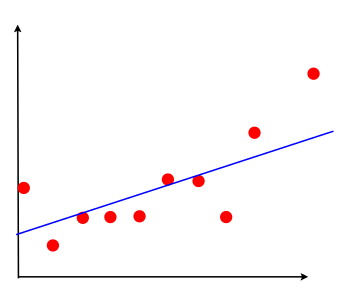
\includegraphics[width=0.6\textwidth, height=5cm]{bias.png}
    \caption[Μοντέλο υψηλής πόλωσης]{Μοντέλο υψηλής πόλωσης}
 \end{figure}
 Η πρώτη επιλογή μας συνιστά μία ευθεία, δηλαδή ένα πολυώνυμο πρώτης τάξης, το οποίο καθορίζεται από δύο παραμέτρους. Παρατηρούμε πως το μοντέλο αυτό είναι τόσο απλό, που όσο και να προσπαθήσουμε δε θα καταφέρει να προβλέψει καλά τα δεδομένα μας. Θα ήταν ουτοπικό να χαρακτηρίζεται κάποιο πραγματικό φαινόμενο από μια τόσο απλή συνάρτηση, οπότε θα απορρίπταμε αυτό το μοντέλο ως υψηλά πολωμένο, καθώς κάνει μια σημαντική υπόθεση απλότητας.
 \begin{figure}[H]
	\centering			
    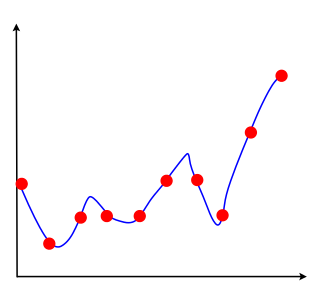
\includegraphics[width=0.6\textwidth, height=5cm]{variance.png}
    \caption[Μοντέλο υψηλής διακύμανσης]{Μοντέλο υψηλής διακύμανσης}
 \end{figure}
 Η δεύτερη επιλογή μας είναι ένα πολυώνυμο υψηλής τάξης, το οποίο μπορεί εύκολα να επιδείξει μηδενικό σφάλμα στα δεδομένα εκπαίδευσης που διαθέτουμε. Το μοντέλο αυτό είναι φαινομενικά τέλειο και αναπόφευκτα προκαλεί αμφιβολίες: είναι όλα τα δεδομένα μας τόσο αξιόπιστα και χαρακτηριστικά για το φαινόμενο που προβλέπουμε, ώστε να αξίζει να τα προσεγγίσουμε τέλεια; Γενικά, δεδομένα πολύ υψηλής διακύμανσης είναι ύποπτα για θόρυβο, ο οποίος ως τυχαίος είναι συχνά υψίσυχνος, σε αντίθεση με φυσικά δεδομένα που υπακούν σε κάποιες συνθήκες ομαλότητας. Μήπως λοιπόν στην προσπάθειά μας να προβλέψουμε καλά την άγνωστη συνάρτηση παρασυρθήκαμε και μοντελοποιήσαμε το θόρυβο; Ένα τέτοιο μοντέλο είναι καταδικασμένο να αποτύχει σε καινούρια δεδομένα και χαρακτηρίζεται ως μοντέλο υψηλής διακύμανσης. Το παραπάνω πρόβλημα είναι αυτό που έχουμε αποκαλέσει υπερπροσαρμογή.
 
Ο θόρυβος, που μας παρασύρει σε υπερπροσαρμογή, αποτελείται από δύο συνιστώσες: το στοχαστικό θόρυβο, ο οποίος κάθεται τυχαία στα δεδομένα μας και χαρακτηρίζεται από μία κατανομή $\epsilon(x)$ και τον ντετερμινιστικό. Ο τελευταίος οφείλεται στην πολυπλοκότητα της συνάρτηση-στόχου: το μοντέλο ερμηνεύει ως θόρυβο οποιαδήποτε διακύμανση δεν μπορεί να μοντελοποιήσει, καθώς είναι πολύ πολύπλοκη για αυτό, είτε αυτή γεννήθηκε τυχαία είτε προήλθε από τη συνάρτηση-στόχο.

Η μαθηματική αποτύπωση του παραπάνω προβλήματος έχει ως εξής: αν επιλέξουμε ένα μοντέλο $g(x)$ για να προβλέψουμε μια συνάρτηση $f(x)$ και ορίσουμε ως $\bar{g(x)}$ την καλύτερη δυνατή πρόβλεψη που μπορεί να κάνει το μοντέλο δεδομένων των παραμέτρων που περιέχει και της πολυπλοκότητας της $f(x)$ και $g_D(x)$ όλες τις πιθανές υποθέσεις που είναι σε θέση να κάνει το μοντέλο, ρυθμίζοντας τις παραμέτρους του, τότε το σφάλμα στο σετ εκπαίδευσης μπορεί να χαρακτηρισθεί ως εξής:
$$E_{error}=\underbrace{E_x(g_D(x) - g(x))^2}_{\text{σφάλμα λόγω  διακύμανσης}} + \underbrace{E_x(g(x)- f(x))^2}_{\text{σφάλμα λόγω πόλωσης}} + E_{\epsilon,x}(\epsilon(x^2))$$
\paragraph{Η ιδέα της κανονικοποίησης} Η τεχνική της κανονικοποίησης στοχεύει στη μείωση της διακύμανσης με ταυτόχρονη διατήρηση χαμηλής πόλωσης. Με απλά λόγια, προσπαθεί να διατηρήσει την πολυπλοκότητα της υπόθεσης, διατηρώντας το
ίδιο πλήθος παραμέτρων, ώστε να έχει τη δυνατότητα να προβλέψει μια πολύπλοκη συνάρτηση-στόχο, περιορίζοντας ωστόσο την επιλογή των τιμών των παραμέτρων, ώστε να δυσκολεύεται να προβλέψει το θόρυβο.
 \begin{figure}[H]
	\centering			
    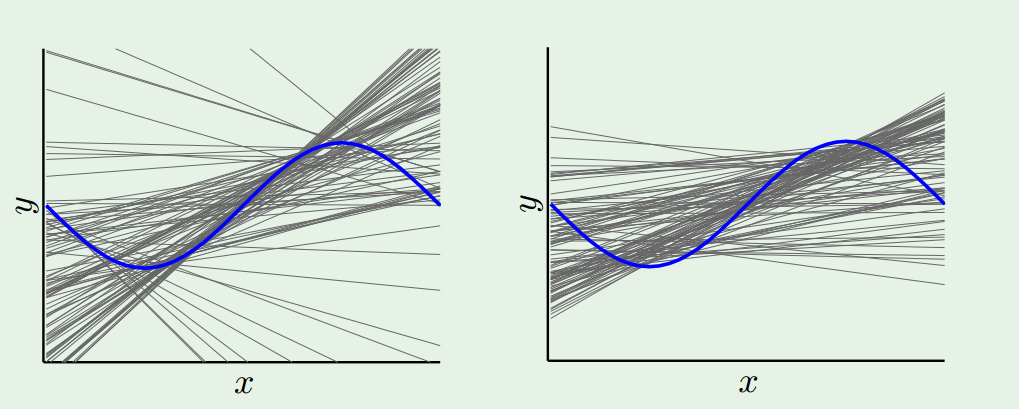
\includegraphics[width=0.8\textwidth]{reg_example.png}
    \caption[Παράδειγμα κανονικοποίησης]{Παράδειγμα κανονικοποίησης: Η άγνωστη συνάρτηση που προσπαθούμε να προβλέψουμε είναι ένα ημίτονο και το μοντέλο που επιλέγουμε είναι το γραμμικό, για χάρη απλότητας. Αριστερά, πριν την κανονικοποίηση, το μοντέλο μας είναι ελεύθερο να επιλέξει οποιαδήποτε ευθεία επιθυμεί. Δεξιά, έχουμε περιορίσει την κλίση και το σταθερό συντελεστή της ευθείας, καταφέρνοντας μικρότερη διακύμανση στις υποθέσεις μας και μικρότερο σφάλμα, καθώς έχουν αποκλειστεί κάποιες πολύ κακές υποθέσεις.}
 \end{figure}
 
Στη συνέχεια θα δούμε πώς εφαρμόζεται η κανονικοποίηση σε ένα πρόβλημα λογιστικής παλινδρόμησης με πολυωνυμικό μοντέλο και θα κατανοήσουμε την επίλυση γραφικά.
 
Όπως έχουμε δει στο κεφάλαιο της λογιστικής παλινδρόμησης, η συνάρτηση λάθους που προσπαθούμε να ελαχιστοποιήσουμε ώστε να βρούμε τη βέλτιστη υπόθεση είναι η εξής:
$$E_{in}(w)=\frac{1}{N} \sum_{n=1}^{N} (w^T z_n  - y_n)^2$$

όπου w είναι οι συντελεστές του μοντέλου, y το διάνυσμα κλάσης και x τα διανύσματα εισόδου των Ν παραδειγμάτων. Η λύση της παραπάνω εξίσωσης είναι:
$$w_{in}=(Z^T \inv{Z} y)$$

Αν ορίσουμε την προσπάθειά μας να περιορίσουμε τις παραμέτρους ως τοποθέτηση ενός άνω φράγματος στο μέτρο των συντελεστών, τότε το αναδιατυπωμένο, κανονικοποιημένο πλέον, πρόβλημα έχει ως εξής:
 \begin{flalign*}
\text{Ελαχιστοποίηση} && E_{in}(w)=\frac{1}{N} (Zw-y)^T (Zw-y)  &&\\
\text{Υπό τον περιορισμό} && w^T w \leq C  &&
\end{flalign*}

Το παραπάνω πρόβλημα καθιστά πρόβλημα βελτιστοποίησης με περιορισμό που περιέχει ανισότητα, επομένως μπορεί να επιλυθεί με πολλαπλασιαστές Lagrane και τη βοήθεια της θεωρίας Karush-Kuhn- Tucker. Ωστόσο η γραφική αναπαράσταση του προβλήματος ενδεχομένως να είναι ενδιαφέρουσα, καθώς θα δώσει καλύτερη κατανόηση της φύσης του.

Όπως έχουμε δει στο κεφάλαιο της λογιστικής παλινδρόμησης, η εξίσωση του σφάλματος έχει τη μορφή ελλειψοειδούς καμπύλης. Ο περιορισμός που θέσαμε ορίζει έναν κύκλο στον οποίο κινούνται τα επιτρεπτά w, με ακτίνα C.
 \begin{figure}[H]
	\centering			
    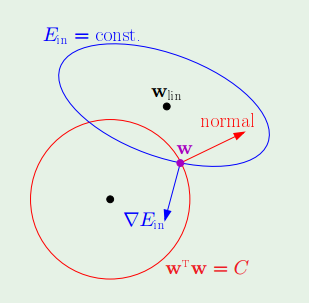
\includegraphics[scale=0.7]{opt_graph.png}
    \caption[Γραφική αναπαράσταση κανονικοποίησης]{Γραφική αναπαράσταση κανονικοποίησης.}
 \end{figure}
 H πληροφορία της κατεύθυνσης προς την οποία πρέπει να κινηθούμε, ώστε να μειώσουμε το $E_{in}$ δίνεται ως γνωστόν από την κλίση, $\nabla E_{in}$ στο σημείο που βρισκόμαστε και φαίνεται στο παραπάνω σχήμα. Όσο αφορά τα w, είναι διανύσματα που κινούνται πιο κοντά γίνεται στη βέλτιστη λύση $w_{lin}$, παραμένοντας βέβαια στον κύκλο. Στο σχήμα φαίνεται πως στην καλύτερη περίπτωση βρίσκονται πάνω στην περιφέρειά του. Παρατηρώ πως, επειδή μεταξύ των δύο διανυσμάτων υπάρχει γωνία, καθώς κινούμαι στον κύκλο, το σφάλμα θα αυξομειώνεται και επομένως δε θα το βελτιστοποιώ. Αντιθέτως, αν το w πάρει την αντίθετη κατεύθυνση από το  $\nabla E_{in}$, θα κινούμαι προς τη βέλτιστη λύση. Επομένως ορίζω τη συνθήκη:
 $$\nabla E_{in}= - 2 \frac{\lambda}{N} w_{reg}$$
 όπου  ως $w_{reg}$ συμβολίζονται οι κανονικοποιημένοι πλέον συντελεστές, $\lambda$ μια σταθερή παράμετρος που επηρεάζει την κανονικοποίηση και N, το γνωστό μας πλήθος παραδειγμάτων.
 
 Σκεπτόμενοι αντιστρόφως από ότι συνήθως, παρατηρούμε πως η παραπάνω εξίσωση μοιάζει με μηδενισμό της παραγώγου μιας συνάρτησης και επομένως θα μπορούσε να αποτελέσει την προσπάθεια βελτιστοποίησης του παρακάτω προβλήματος:
 $$E_{in} + \frac{\lambda}{N} w^T_{reg} w_{reg}=0$$
 
 Η παραπάνω διατύπωση είναι αποκαλυπτική: ένα πρόβλημα βελτιστοποίησης υπό συνθήκη αναδιατυπώθηκε ως ένα απλό πρόβλημα βελτιστοποίησης μιας συνάρτησης, που αντικαθιστώντας με τη γνωστή μας συνάρτηση του $E_{in}$ εκφράζεται ως:
 $$E_{in}(w)=\frac{1}{N}(Zw-y)^T(Zw-y) + \frac{\lambda}{N} w^T_{reg} w_{reg} $$
 
 Με τη ίδια λογική, που είχαμε επιλύσει το πρόβλημα χωρίς κανονικοποίηση, το ψευδοαντίστροφο, η λύση προκύπτει ως:
 $$w_{lin}=\inv{ (Z^T Z)} Z^T y$$
 
 Αν και είδαμε την εφαρμογή της κανονικοποίησης σε ένα συγκεκριμένο μοντέλο, μπορούμε να κατανοήσουμε τη συνολική διαδικασία ως εξής:
 
 $$E_{aug}(h)= E_{in}(h) + \frac{\lambda}{N} \Omega(h)=0$$
 
όπου ως $E_{in(h)}$ συμβολίζουμε το σφάλμα μιας υπόθεσης πριν την κανονικοποίηση και $E_{aug}(h)$ το επαυξημένο σφάλμα, δηλαδή έπειτα από την κανονικοποίηση. Η συνάρτηση $\Omega(h)$ εκφράζει τον τρόπο που θα γίνει η κανονικοποίηση και, ανεξάρτητα από το μοντέλο, έχει ως στόχο την επιβολή περιορισμών που εξασφαλίζουν ομαλότητα ή/και χαμηλότερη πολυπλοκότητα της υπόθεσης.
\paragraph{Η επίδραση της παραμέτρου λ}
Αν η συνάρτηση $\Omega(h)$ εκφράζει τον τρόπο, τότε το $\lambda$ εκφράζει το μέγεθος της κανονικοποίησης.
 \begin{figure}[H]
	\centering			
    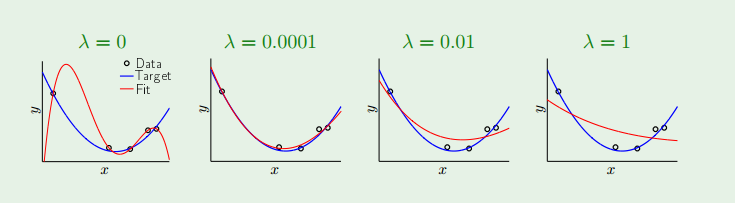
\includegraphics[width=0.8\textwidth]{l_reg.png}
    \caption[Επίδραση λ στην κανονικοποίηση]{Επίδραση λ στην κανονικοποίηση.}
 \end{figure}
 
 Όπως παρατηρούμε στο παραπάνω διάγραμμα υποπεριπτώσεων, επιβολή μικρής τιμής $\lambda$, αντιστοιχεί σε μεγάλο C, δηλαδή ασθενή περιορισμό του μοντέλου, που συνεχίζει να κινδυνεύει από υπερπροσαρμογή. Καθώς αυξάνουμε την τιμή του $\lambda$ γινόμαστε αυστηρότεροι, με κίνδυνο να είμαστε τόσο περιοριστικοί με το μοντέλο που θα οδηγηθούμε σε υπόθεση υψηλής πόλωσης.
 \section{Αυτοματοποιήμενη μηχανική μάθηση (Automl)}
 Έχοντας ρίξει μια φευγαλέα ματιά στην απύθμενη επιστήμη της μηχανικής μάθησης, μάλλον μας έχει δοθεί η εντύπωση πως απευθύνεται σε μια ελιτίστικη κοινωνία ειδικών, που με χρόνια εμπειρίας, εξειδικευμένη έρευνα και λίγη δόση τύχης, καταφέρνει να σχεδιάσει μοντέλα που έχουν μια κάποια χρησιμότητα στον
πραγματικό κόσμο. Είναι αλήθεια πως σε κάθε στάδιο, οι σχεδιαστικές επιλογές που επηρεάζουν την απόδοση του μοντέλου φαίνονται να προέρχονται από έναν άπειρο χώρο και η καλύτερη επιλογή είναι χρονοβόρα και αμφισβητήσιμη. Τα οφέλη ωστόσο που προσφέρει ένα αποδοτικό μοντέλο είναι τόσο άμεσα και το πεδίο εφαρμογών της μηχανικής μάθησης τόσο ευρύ, που η ιδέα της αυτοματοποίησης της διαδικασίας βελτιστοποίησης έχει κινητοποιήσει μια μεγάλη μερίδα ειδικών. Είναι χαρακτηριστικό
το γεγονός ότι στη συνολική διαδικασίας της μηχανικής μάθησης, που ουσιαστικά αφορά την εύρεση του μοντέλου πρόβλεψης, το $75\%$ αφορά την προετοιμασία των δεδομένων και το $15\%$ την ανάλυση των αποτελεσμάτων.

Ο όρος automl είναι σχετικά πρόσφατος στη βιβλιογραφία και αφορά κάθε προσπάθεια
αυτοματοποίησης οποιουδήποτε σταδίου της διαδικασίας της μηχανικής μάθησης. Η ιδέα είναι απλή και μάλλον φανερώνει την επαγωγική φύση του ανθρώπου: ας εκπαιδεύσουμε μία μηχανή που θα εκπαιδεύει μοντέλα πρόβλεψης.
\subsection{Ιστορική Αναδρομή}
Ο τομέας της αυτοματοποίησης της μηχανικής μάθησης βρίσκεται σε πειραματικό στάδιο, όχι όμως και σε εμβρυικό. Τα σύγχρονα, εντυπωσιακά εργαλεία που έχουν στη διάθεσή τους σήμερα οι ειδικοί, προέκυψαν από την εικοσαετή εκκόλαψη της ιδέας της αυτοματοποίησης των βασικών σταδίων της μηχανικής μάθησης. To 1995 η εταιρία Unica εισήγαγε στην αγορά το Pattern Recognition Workbench, ένα πακέτο λογισμικού
που ενσωμάτωσε την αυτομαποίηση της ρύθμισης μοντέλων με νευρωνικά δίκτυα. Το λογισμικό Model 1 αποτέλεσε απόγονο του παραπάνω προϊόντος, καθώς το επέκτεινε και σε άλλες οικογένειες αλγορίθμων. Τα τέλη της δεκαετίας του 90 έχουν να επιδείξουν ακόμη δύο προσπάθειες: το Marketswitch, και το KXEN, εργαλεία που απευθύνονταν κυρίως στην αγορά του Marketing, παρέχοντας διεπαφές για αυτοματοποίηση των προβλεπτικών μοντέλων. Πιο πρόσφατα παραδείγματα αποτελούν οι κολοσσοί στην αγορά των πωλητών λογισμικού για στατιστικές αναλύσεις: η SAS και η IBM SPSS με τα προιόντα τους SAS Rapid Modeler και IBM SPSS Modeler αντίστοιχα, προσπάθησαν από το 2010 να αυτοματοποιήσουν την προ επεξεργασία των δεδομένων, παραχωρώντας ταυτόχρονα στο χρήστη λειτουργικότερες διεπαφές.

Αν και βραχύβια, η ιστορία του automl μπορεί να μας διδάξει κάτι: η αρχική θεώρηση της αυτοματοποίησης της μηχανικής μάθησης ως λύτρωση  από τη χρονοβόρα και πνευματικά απαιτητική επίτευξη ενός αποτελεσματικού μοντέλου ήταν λανθασμένη. Τα εργαλεία που αντιμετώπισαν την εκπαίδευση ως ένα μαύρο κουτί, ώστε ο χρήστης να πετυχαίνει εντυπωσιακά αποτελέσματα αγνοώντας τις βασικές αρχές και λειτουργίες των αλγορίθμων, απέτυχε κατά την εφαρμογή της σε πραγματικά προβλήματα. Πλέον αντιλαμβανόμαστε αυτόν τον τομέα ως ένα εργαλείο στα χέρια του ειδικού, που επιταχύνει, διευκολύνει και επεκτείνει τη μηχανική μάθηση, όπως ένα  εργαλείο ρομποτικής ιατρικής στα χέρια ενός χειρούργου. 

\subsection{Χρήση σε βελτιστοποίηση υπερπαραμέτρων}
Κατά την εκπαίδευση του μοντέλου ο αναλυτής καλείται να επιλέξει διάφορες υπερπαραμέτρους που χαρακτηρίζουν το σετ υπόθεσης και παραμέτρους που επηρεάζουν τον αλγόριθμο εκπαίδευσης. Επομένως, απαιτούνται αρκετά πειράματα, ώστε με επαλήθευση να διαπιστωθεί ποιες παράμετροι δίνουν το καλύτερο αποτέλεσμα. Τεχνικές όπως η τυχαία αναζήτηση ή η αναζήτηση σε κάποιο πλέγμα παραμέτρων είναι χρονοβόρες, δεν παρέχουν καμία εγγύηση εύρεσης ολικού μεγίστου, όσο αφορά τη συνάρτηση απόδοσης, και για περίπλοκα μοντέλα, όπως τα deep belief networks, είναι απαγορευτικές.

Η αυτοματοποίηση αυτού του σταδίου καταλαμβάνει μεγάλο μέρος της βιβλιογραφίας της επιστήμης του Automl, καθώς αποτελεί το πιο περίπλοκο και σημαντικό κομμάτι της διαδικασίας της μηχανικής μάθησης.

\subsubsection{Bayesian βελτιστοποίηση}
\paragraph{Βελτιστοποίηση blackbox συναρτήσεων} Η αναζήτηση των βέλτιστων παραμέτρων γίνεται με άξονα τη μεγιστοποίηση της γενικευμένης απόδοσης: ενός δείκτη που δηλώνει πόσο καλά δουλεύει το μοντέλο μας σε άγνωστα δεδομένα, δηλαδή πόσο κοντά έχει πέσει η υπόθεσή μας στην πραγματική συνάρτηση, που περιγράφει πώς προκύπτει η υπό μελέτη κλάση από τα χαρακτηριστικά. Η συνάρτησή αυτή μας είναι άγνωστη: δεν έχουμε λόγο να πιστεύουμε πως είναι γραμμική ή κυρτή, άρα η εύρεση ενός τοπικού μεγίστου δεν εξασφαλίζει και εύρεση ολικού. Επίσης, δεδομένου του ότι έχουμε να κάνουμε με πραγματικά προβλήματα, η συνάρτηση που προσπαθούμε να προσεγγίσουμε μάλλον είναι περίπλοκη. Το μόνο που γνωρίζουμε για αυτήν είναι τα δεδομένα που έχουμε, δηλαδή κάποιες εισόδους και εξόδους της, εξού και ο χαρακτηρισμός της ως μαύρο κουτί. Τα δεδομένα που έχουμε είναι μάλιστα περιορισμένα, καθώς η απόκτησή τους μπορεί να απαιτεί χρόνο, κόπο και χρήματα (δοκιμές φαρμάκων, οικονομικές επενδύσεις). Η βελτιστοποίηση μιας συνάρτησης f(x) με παραμέτρους από ένα σύνολο A, συμβολίζεται ως:
$$\max_{x \in \subset R^d } f(x)$$
Ο όρος Bayesian βελτιστοποίηση εισήχθη από τον Jonas Mockus τη δεκαετία του 70 σε μια σειρά μελετών του για ολική βελτιστοποίηση συναρτήσεων. Βασικά χαρακτηριστικά αυτής της διαδικασίας είναι πως είναι ακολουθιακή, ενσωματώνει κάποια εκ των προτέρων πεποίθηση που έχουμε για την υπό βελτιστοποίηση συνάρτηση, χρησιμοποιεί το θεώρημα Bayes και καθοδηγεί την αναζήτηση του μεγίστου με βάση ένα συνδυασμό μεταξύ εξερεύνησης και εκμετάλλευσης.Ας τα πάρουμε όμως με τη σειρά.
\paragraph{Θεώρημα Bayes} Σύμφωνα με αυτό το θεώρημα, δεδομένου ενός μοντέλου πρόβλεψης M και ενός συνόλου παρατηρήσεων Ε, η εκ των υστέρων πιθανότητα, δηλαδή η πιθανότητα δεδομένων των παρατηρήσεων Ε να προκύψει το μοντέλο M είναι ανάλογη της πιθανότητας των παρατηρήσεων δεδομένου του μοντέλου επί την εκ των προτέρων πιθανότητα του μοντέλου, με μαθηματικούς όρους:
$$P(M \mid E) \propto P(E \mid M) \cdot P(M) $$
Η παραπάνω πιθανότητα μας δίνει ένα μέσο για να απαντήσουμε στο πραγματικό ερώτημα: ”Δεδομένων των παρατηρήσεων που έχω στη διάθεσή μου, ποιο μοντέλο είναι πιθανότερο να προσεγγίζει καλύτερα την πραγματική συνάρτηση;”
\paragraph{Η Γκαουσιανή διαδικασία ως εκ των προτέρων πιθανότητα} Η εκ των προτέρων πιθανότητα αντικατοπτρίζει την πεποίθηση που έχουμε για την άγνωστη συνάρτηση. Αν πιστεύουμε για παράδειγμα πως ένα χαρακτηριστικό της είναι η ομαλότητα, αυτομάτως κάποιες συναρτήσεις γίνονται πιο πιθανές από άλλες.

Η γκαουσιανή διαδικασία ορίζεται ως μια επέκταση μιας γκαουσιανής κατανομής πολλών μεταβλητών σε μια στοχαστική διαδικασία απείρων διαστάσεων, όπου κάθε πεπερασμένος συνδυασμός διαστάσεων δίνει μια γκαουσιανή κατανομή. Όπως ακριβώς η γκαουσιανή κατανομή δίνει την κατανομή κάποιων μεταβλητών και χαρακτηρίζεται πλήρως από τη μέση τιμή και τη διακύμανσή της, έτσι και η γκαουσιανή διαδικασία αποτελεί μια κατανομή συναρτήσεων που χαρακτηρίζεται από κάποια μέση
συνάρτηση και μια συνάρτηση διακύμανσης. Για να κατανοήσουμε καλύτερα τη διαδικασία αυτή, μπορούμε να σκεφτούμε πως όπως μία συνάρτηση επιστρέφει έναν αριθμό $f(x)$ για μία τιμή x, αυτή επιστρέφει τη μέση τιμή και διακύμανση μιας κανονικής κατανομής, που δίνει όλες τις πιθανές τιμές της $f(x)$ για το συγκεκριμένο x.
\paragraph{Συνάρτηση απόκτησης} Έχοντας κάποια στοιχεία της συνάρτησης και γνωρίζοντας την πιθανότητα ενός μοντέλου δεδομένων αυτών, πως θα επιλέξω τις επόμενες τιμές των παραμέτρων που θα δοκιμάσω; Προς αυτό το σκοπό χρησιμοποιούνται οι συναρτήσεις απόκτησης που μεγιστοποιούνται για σημεία που
ενδεχομένως να μεγιστοποιούν και την άγνωστη συνάρτηση. Υπάρχουν διάφορες τεχνικές, ωστόσο η βασική αρχή επιλογής αποτελεί ένα συμβιβασμό μεταξύ ''εξερεύνησης'' και ''εκμετάλλευσης'': θέλουμε να κινηθούμε προς περιοχές για τις οποίες γνωρίζουμε ήδη πως το μοντέλο λειτουργεί καλά χωρίς ωστόσο να αποκλείουμε ανεξερεύνητες περιοχές, προκειμένου να αποφευχθεί ο κίνδυνος εμμονής σε κάποιο τοπικό μέγιστο.
\begin{itemize}
\item \textit{Πιθανότητα βελτίωσης.} Μία από τις πρώτες τεχνικές, που εισήχθη από τον Kushner το 1964, ήταν αυτή της επιλογής του σημείου $x^+$ με τη μεγαλύτερη πιθανότητα βελτίωσης:
$$PI(x)= P(f(x) \geq f(x^+)) = \Phi (\frac{\mu(x) - f(x^+)}{\sigma(x)})$$

όπου $\Phi$ είναι η συνάρτηση κανονικής αθροιστικής κατανομής.

Το βασικό της μειονέκτημα τότε ήταν ότι δεν λάμβανε καθόλου υπόψιν της το στοιχείο της εξερεύνησης, το οποίο εισήχθη μέσω της παραμέτρου $\xi$ ως εξής:
$$PI(x)= P(f(x) \geq f(x^+)) = \Phi (\frac{\mu(x) - f(x^+) - \xi}{\sigma(x)})$$

Η εισαγωγή της παραμέτρου $\xi$ έλυσε μεν το πρόβλημα, δίνοντας ένα αντιληπτό κατώφλι στη βελτίωση που επιτυγχάνεται, αποτελεί δε μια σημαντική σχεδιαστική επιλογή, που οδηγεί εύκολα σε σφάλμα, καθώς για ακατάλληλα μικρή τιμή υπάρχει ο κίνδυνος εγκλωβισμού σε τοπικό μέγιστο, ενώ για μεγάλη τιμή η διαδικασία θα γίνει πολύ αργή.

Μία πιο ικανοποιητική προσέγγιση θα ήταν κατά την επιλογή του επόμενου σημείου να μη ληφθεί υπόψιν μόνο η πιθανότητα βελτίωσης, αλλά και το μέγεθος της βελτίωσης. Πιο συγκεκριμένα, θα θέλαμε να ελαχιστοποιήσουμε την προσδοκώμενη απόκλιση από το πραγματικό μέγιστο:
$$x_{t+1}= argmin E(\abs{f_{t+1}(x) -f(x^*)} D_{1:t})$$

O Mockus όρισε με πολύ πρακτικό τη συνάρτηση βελτίωσης ως εξής:
$$I(x)= \max ( f_{t+1} (x) - f(x^*)$$
δηλαδή η βελτίωση είναι θετική όταν η πρόβλεψη είναι μεγαλύτερη από την μέχρι τώρα καλύτερη τιμή, ειδάλλως μηδέν. Το νέο σημείο βρίσκεται μεγιστοποιώντας την προσδοκώμενη βελτίωση:
$$x=argmax(E( \max( f_{t+1}(x) - f(x^*) \mid D_t))$$
H πιθανότητα διαπίστωσης βελτίωσης I σε μία κανονική κατανομή, που χαρακτηρίζεται από μέση τιμή $\mu(x)$ και διακύμανση $\sigma(x)^2$ υπολογίζεται ως εξής:
$$ \frac{1}{\sqrt[]{2 \pi} \sigma(x)} e^{- \frac{(\mu(x)- f(x^*-I))^2}{s \cdot \sigma(x)^2}}$$
και η προσδοκώμενη βελτίωση είναι το ολοκλήρωμα της παραπάνω συνάρτησης ως προς I.
\item \textit{Χρήση άνω ορίων εμπιστοσύνης.} Στην τεχνική αυτή είναι ξεκάθαρη η προσπάθεια συμβιβασμού εξερεύνησης και εκμετάλλευσης. Όπως έχουμε αναφέρει, η μέση τιμή της γκαουσιανής διαδικασίας αποτελεί την τρέχουσα εντύπωση που έχουμε για την άγνωστη συνάρτηση. Μπορούμε να επιλέξουμε πόσο εξερευνητικοί θα είμαστε ορίζοντας πόσες τυπικές αποκλίσεις πέρα από τη μέση τιμή της διαδικασίας θα κινηθούμε.
\end{itemize}
Παρακάτω παρατηρούμε την οπτικοποίηση της bayesian βελτιστοποίησης:
\begin{figure}[H]
\begin{minipage}[c][11cm][t]{.5\textwidth}
  \vspace*{\fill}
  \centering
  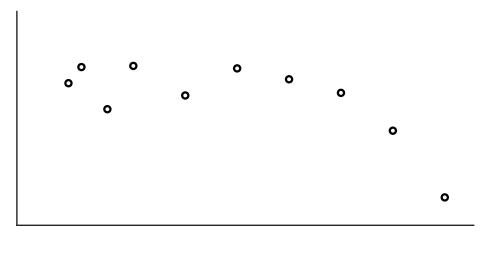
\includegraphics[width=5cm,height=3cm]{sample.png}
  \caption[Αρχικό δείγμα υπερπαραμέτρων]{Αρχικό δείγμα υπερπαραμέτρων}
 \label{fig:test2}\par\vfill
  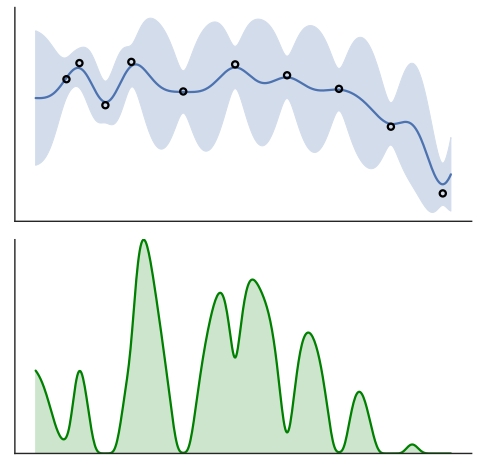
\includegraphics[width=5cm,height=3cm]{explore.png}
  \caption[Συνάρτηση απόκτησης]{Συνάρτηση απόκτησης: παρατηρούμε την προσπάθεια εξερεύνησης περιοχών χωρίς δείγματα με ταυτόχρονη προσέγγιση καλών δειγμάτων}
  
\end{minipage}
\begin{minipage}[c][11cm][t]{.5\textwidth}
  \vspace*{\fill}
  \centering
  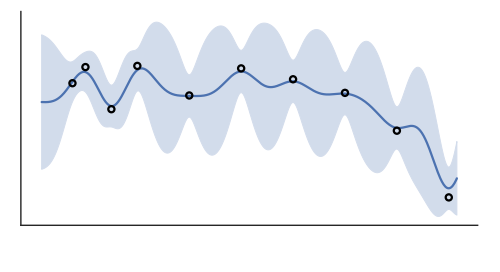
\includegraphics[width=5cm,height=3cm]{posterior.png}
  \caption[Προσαρμογή μοντέλου στο δείγμα με βάση την εκ των υστέρων πιθανότητα]{Προσαρμογή μοντέλου στο δείγμα με βάση την εκ των υστέρων πιθανότητα με χρήση γκαουσιανών συναρτήσεων }
  \label{fig:test2}\par\vfill
  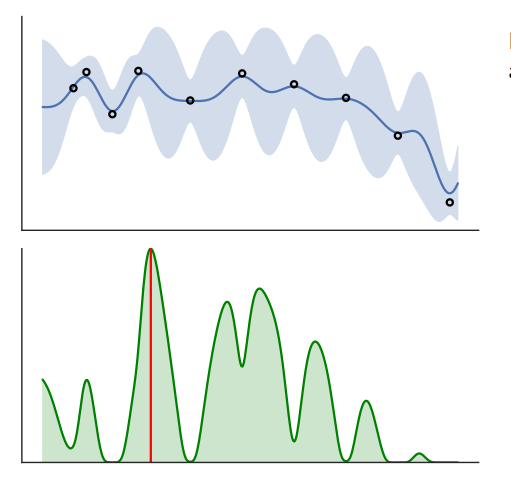
\includegraphics[width=5cm,height=3cm]{optimize.png}
  \caption[Βελτιστοποίηση συνάρτησης απόκτησης]{Βελτιστοποίηση συνάρτησης απόκτησης }
\end{minipage}
\begin{minipage}[c][5cm][t]{\textwidth}
  \centering
  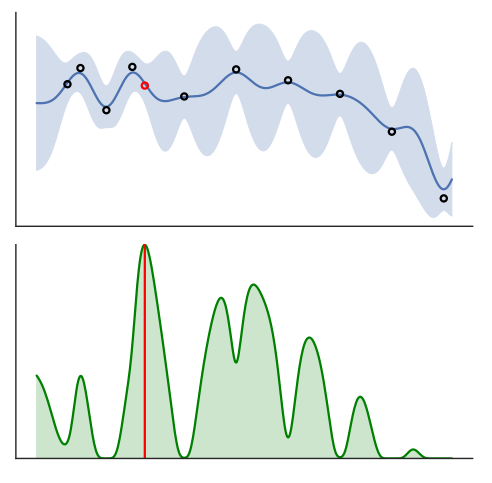
\includegraphics[width=5cm,height=3cm]{next.png}
  \caption[Επιλογή επόμενου σημείου δειγματοληψίας ]{Επιλογή επόμενου σημείου δειγματοληψίας ως αυτό που βελτιστοποίησε τη συνάρτηση απόκτησης.}
  \label{fig:test2}\par\vfill
\end{minipage}
\end{figure}
\subsubsection{Ακολουθιακή βελτιστοποίηση βασισμένη σε μοντέλο (SMBO)}
Το πρόβλημα της βελτιστοποίησης υπερπαραμέτρων μπορεί να διατυπωθεί επισήμως ως εξής: \textit{Δεδομένου ενός παραμετροποιημένου αλγορίθμου Α, ενός συνόλου παραδειγμάτων I και μίας μετρικής κόστους c, να βρεθούν οι υπερπαράμετροι του Α που ελαχιστοποιούν το c στο Ι.} Η μετρική c μπορεί να αφορά είτε την ταχύτητα του αλγορίθμου είτε την ποιότητα του αποτελέσματος. Οι λύσεις που έχουν δοθεί στο παραπάνω πρόβλημα ανήκουν κυρίως σε δύο κατηγορίες: αυτές που χρησιμοποιούν ένα μοντέλο εκπαίδευσης για την εύρεση των βέλτιστων υπερπαραμέτρων και αυτές που το καταφέρνουν χωρίς τη χρήση του.

Στη δεύτερη κατηγορία συναντούμε απλούς αλγορίθμους, που βασίζονται σε τεχνικές όπως η τυχαία, ομοιόμορφη  αναζήτηση στο πλέγμα των υπερπαραμέτρων (\textit{ROAR}), επαναληπτική τοπική αναζήτηση(\textit{PARAMILS}) και γενετικούς αλγορίθμους (\textit{GGA}). Θα λέγαμε ότι αποτελούν την πρώτη γενιά  αλγορίθμων ακολουθιακής βελτιστοποίησης.

Οι αλγόριθμοι βελτιστοποίησης που χρησιμοποιούν μοντέλα εκπαίδευσης εκκολάφτηκαν από τη διαπίστωση πως η συνάρτηση, $f: \Theta \rightarrow Y$ που καθορίζει πως επιδρούν οι παράμετροι στην απόδοση του μοντέλου είναι περίπλοκη και οφείλει να προσεγγιστεί από κάποιο μοντέλο μηχανικής μάθησης. Έτσι, τα δεδομένα εκπαίδευσης έχουν τη μορφή ${(\theta_1,y_1),...,(\theta_n,y_n)}$, όπου $\theta_i=(\theta_{i,1}..., \theta_{i,d})$ οι d παράμετροι και $y_i$ η απόδοση που επιτεύχθει με αυτές. Ένας τυπικός αλγόριθμος αυτής της κατηγορίας περιέχει έναν εσωτερικό βρόγχο, όπου επιλέγουμε το σημείο $x^*$, που βελτιστοποιεί την πρόβλεψη, ως το επόμενο σημείο αξιολόγησης της f. Οι αλγόριθμοι διαφοροποιούνται ως προς το κριτήριο που χρησιμοποιούν για να βελτιστοποιήσουν την πρόβλεψη και ποιο μοντέλο εκπαίδευσης χρησιμοποιούν.
\begin{myalgorithm}[H]
H=0\;
 \For{t=1 μέχρι Τ }{
  βρες τo $\theta^*=argmin S(\theta, M_{t-1})$ \;
  υπολόγισε το $f(\theta^*)$\;
  Ανανέωσε το σετ εκπαίδευσης $H=H \cup (\theta^*, f(\theta^*)) $\;
  Εκπαίδευσε ένα νέο μοντέλο $M_t$ στο Η \;
 }
 \caption{Γενικός Ψευδοκώδικας SΜΒΟ}
\end{myalgorithm}
\paragraph{Ακολουθιακή ρύθμιση αλγορίθμου βασισμένη σε μοντέλο (SMAC)} Ο αλγόριθμος αυτός αποτελεί χαρακτηριστικό παράδειγμα αυτής της οικογένειας. Παρουσιάστηκε το 2011 από τους Frank Hutter, Holger Hoos και Kevin Leyton-Brown. Χρησιμοποιεί instance-based μοντέλα , όπως γκαουσιανά  μοντέλα ακτινικής βάσης, αλλά και δέντρα, όπως τον αλγόριθμο Random Forest. Το κριτήριο επιλογής που χρησιμοποιεί είναι αυτό της προσδοκώμενης βελτίωσης, που αναλύσαμε στο προηγούμενο κεφάλαιο και ορίζεται ως:
$$EI(\theta)_{y^*} (\theta)= \int_{- \infty}^{y^*} (y^* - y) p(y \mid \theta) dy$$ 
\paragraph{Δέντρο εκτιμητών Parzen (TPE)}
Ενώ ο αλγόριθμος SMAC υπολογίζει απευθείας την ποσότητα $p(y \mid \theta)$ κατά την εύρεση της προσδοκώμενης βελτίωσης, εδώ θα την προσεγγίσουμε με τη βοήθεια των  $p(\theta \mid y)$ και $ p(y)$. Συγκεκριμένα, μοντελοποιούμε την πιθανότητα $p(\theta \mid y)$ ως μία εκ δύο εκτιμήσεων πυκνότητας, ανάλογα με το αν η απόδοση y έχει ξεπεράσει κάποιο κατώφλι $y^*$:
$$p(\theta \mid y)=\left\{
	\begin{array}{ll}
		l(\theta)  & \mbox{if } y < y^* \\
		g(\theta)  & \mbox{if } y \geq y^*
	\end{array}
\right.$$

Το σημείο $y^*$ επιλέγεται με τη χρήση μιας παραμέτρου γ, ώστε να αντιστοιχεί στο γ-μόριο των απωλειών του TPE αλγορίθμου μέχρι την παρούσα στιγμή. Η συνάρτηση $l(\theta)$ είναι μια κατανομή που προήλθε από όλες τις προηγούμενες υπερπαραμέτρους θ που οδήγησαν σε σφάλμα μικρότερο από $y^*$ και η $g(\theta)$ από τις υπόλοιπες. Έτσι, μπορούμε να ερμηνεύσουμε την πρώτη ως μία εκτίμηση της κατανομής των υπερπαραμέτρων που έχουν καλή απόδοση, έναντι αυτών που παρουσιάζουν φτωχή απόδοση.
\fbox{\begin{minipage}{\textwidth}
\begin{center}
Parzen Εκτιμητής
\end{center} 
Το μαθηματικό αυτό εργαλείο ανακαλύφθηκε από τον Emmanuel Parzen στις αρχές του 1960 και έχει βρει εφαρμογή σε πολλά πεδία, όπως αυτό της μηχανικής μάθησης. Το παράθυρο του Parzen για  εκτίμηση της πυκνότητας, όπως είναι η επίσημη ονομασία του, αποτελεί ουσιαστικά μία μέθοδο παρεμβολής. Για ένα τυχαίο δείγμα x, η τεχνική αυτή υπολογίζει την συνάρτηση πυκνότητας PDF(x) τοποθετώντας συναρτήσεις πυρήνα, συνήθως την γκαουσιανή, στις υπόλοιπες παρατηρήσεις και αθροίζοντας τη συνεισφορά τους στο συγκεκριμένο σημείο.
\end{minipage}}
\\

Οι κατανομές $l(\theta)$ και $g(\theta)$ παρουσιάζουν μία ιεραρχική δομή, καθώς αντιπροσωπεύουν τις υπερπαραμέτρους και τη συσχέτιση μεταξύ τους. Όσο αφορά τις υπερπαραμέτρους με συνεχείς τιμές, μπορούμε να φανταστούμε πως έχουμε  υπολογίσει τον Parzen εκτιμητή για κάθε μια από αυτές. Για να υπολογίσουμε την πιθανότητα ενός παραδείγματος υπερπαραμέτρων $\theta$, ξεκινούμε από την κορυφή του δέντρου και κατευθυνόμαστε προς τα φύλλα ακολουθώντας τις υπερπαραμέτρους που έχουμε. Η πιθανότητα σε κάθε κόμβο αντιστοιχεί στον Parzen εκτιμητή και τους συνδυάζουμε ακολουθώντας την αντίθετη διαδρομή προς τη ρίζα.

Τελικά, το κριτήριο που μεγιστοποιείται είναι:
$$EI(I_{y_{min}}(\theta)) \propto (\gamma + \frac{g(\theta)}{l(\theta)} \cdot (1- \gamma))^{-1}  $$

δοκιμάζοντας διάφορους υποψήφιους συνδυασμούς των υπερπαραμέτρων και επιλέγοντας αυτόν με τη μικρότερη τιμή $g(\theta)/l(\theta)$.

\subsection{Σύγχρονα εργαλεία automl}
Αν αναλογιστεί κανείς το εύρος των εφαρμογών μηχανικής μάθησης, θα κατανοήσει την ύπαρξη πληθώρας εργαλείων που επιχειρούν να την αυτοματοποιήσουν. Βιβλιοθήκες σε διάφορες γλώσσες, παρέχουν διεπαφές προς τεχνικές αυτοματοποίησης, διαδικτυακά περιβάλλοντα,  αναλαμβάνουν τη διαιτησία ολόκληρης της διαδικασίας της μηχανικής μάθησης, προσφέροντας δυνατότητες αυτόματης βελτιστοποίησης της και λογισμικά εξειδικευμένα στην ανάλυση δεδομένων ενσωματώνουν διεπαφές προς υλοποιημένους αλγορίθμους βελτιστοποίησης. Η εμπορική σημασία της αυτόματης επίτευξης μοντέλων πρόβλεψης έχει οδηγήσει στην κυκλοφορία πολλών εμπορικών εργαλείων, αλλά και οι κοινότητες ελεύθερου λογισμικού έχουν κινητοποιηθεί μπροστά σε αυτήν την πολύπλευρη ανάγκη. Στη συνέχεια θα δούμε μερικά χαρακτηριστικά εργαλεία.
\paragraph{HPOlib} Πρόκειται για μία βιβλιοθήκη βελτιστοποίησης υπερπαραμέτρων, που παρέχει μία κοινή διεπαφή προς τρία σύγχρονα, αναγνωρισμένα πακέτα: 
\begin{itemize}
\item \textit{ SMAC.}
\item \textit{ Spearmint.} Γραμμένο σε python, χρησιμοποιείται για την εφαρμογή bayesian βελτιστοποίησης.
\item \textit{ Hyperopt.} Γραμμένο σε python, αναλαμβάνει τη βελτιστοποίηση σε ιδιαίτερους χώρους αναζήτησης με τη χρήση τυχαία αναζήτησης και του αλγορίθμου TPE.
\end{itemize}
\paragraph{Autoweka} Το Waikato Environment for Knowledge Analysis(Weka) είναι ένα λογισμικό σχετικό με τους τομείς της ανάλυσης δεδομένων και μοντέλων πρόβλεψης. Υλοποιεί πληθώρα αλγορίθμων μηχανικής μάθησης, γραμμένων σε Java και παρέχει γραφικές διεπαφές και εργαλεία οπτικοποίησης για διευκόλυνση των χρηστών. Το λογισμικό αυτό έχει ενσωματώσει την αυτοματοποίηση της μηχανικής μάθησης στο Autoweka, που εισήχθη το 2013 και αναλαμβάνει την επίλυση του προβλήματος της συνδυασμένης επιλογής αλγορίθμου και βελτιστοποίησης υπερπαραμέτρων (CASH). Συνεχίζοντας την παράδοση του εργαλείου αυτού στην απλότητα χρήσης, το Autoweka αντιμετωπίζεται ως ένας απλός αλγόριθμος μάθησης, που αναλαμβάνει την επιλογή των χαρακτηριστικών, του μοντέλου και  τη βελτιστοποίηση των υπερπαραμέτρων, ανάμεσα σε όλες τις τεχνικές και αλγορίθμους που προσφέρει το Weka. Για να επιλύσει αυτό το τρομακτικά πολυδιάστατο πρόβλημα έχει βασιστεί σε SMBO αλγορίθμους (SMOC, TPE).  
\paragraph{Πακέτο Caret} Το πακέτο αυτό ανήκει στην R, που αποτελεί μία γλώσσα προγραμματισμού και ένα περιβάλλον λογισμικού εξειδικευμένο στη στατιστική. Η R είναι το κατεξοχήν εργαλείο για συγγραφή κώδικα σε εφαρμογές στατιστικής, ανάλυσης δεδομένων και μηχανικής μάθησης και  διαθέτει πακέτα που επιτελούν πληθώρα αλγορίθμων και τεχνικών, καθώς και εργαλείων οπτικοποίησης. Οι κοινότητες ελεύθερου λογισμικού έχουν εξοπλίσει την R με πακέτα που επιχειρούν τη βελτιστοποίηση της μηχανικής μάθησης, όπως αυτόματης προ επεξεργασίας δεδομένων και  ρύθμισης μοντέλου, οι διεπαφές των οποίων είναι αναμενόμενα ανομοιόμορφες.  Το πακέτο caret(classification and regression training) αποτελεί προσπάθεια τυποποίησης της διαδικασίας της εκπαίδευσης παρέχοντας ομοιόμορφες διεπαφές και  εργαλεία για διαχωρισμό των δεδομένων, προ επεξεργασία, επιλογή χαρακτηριστικών, ρύθμιση των παραμέτρων του μοντέλου, εκτίμηση της σημασίας των χαρακτηριστικών και άλλων λειτουργιών χρήσιμων στην προσπάθεια αυτοματοποίησης της εκπαίδευσης ενός μοντέλου.
\begin{figure}[H]
\begin{minipage}[c][11cm][t]{.5\textwidth}
  \vspace*{\fill}
  \centering
  
\includegraphics[width=5cm,height=3cm]{weka_1.png}
  \caption[Weka]{Weka}
  \label{fig:test2}\par\vfill
  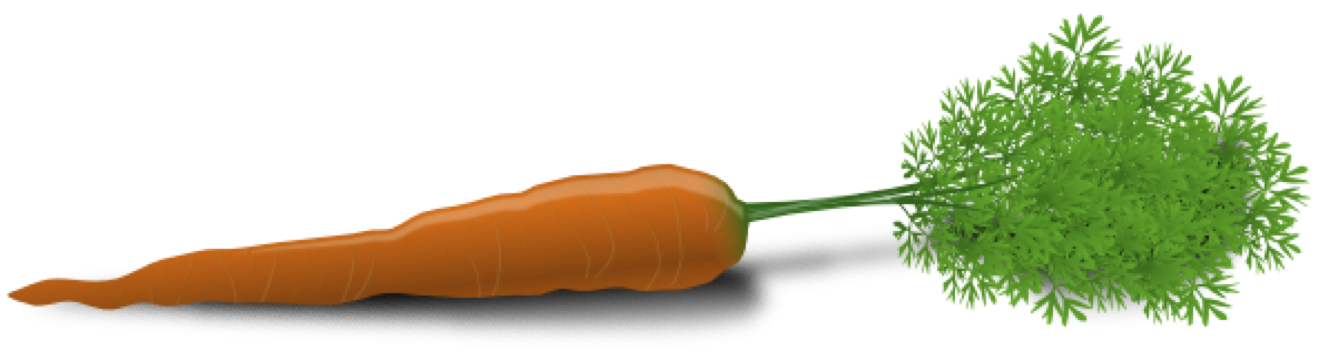
\includegraphics[width=5cm,height=3cm]{caret_1.png}
  \caption[Πακέτο Caret]{Πακέτο Caret}
  \label{fig:test3}
\end{minipage}
\begin{minipage}[c][11cm][t]{.5\textwidth}
  \vspace*{\fill}
  \centering
  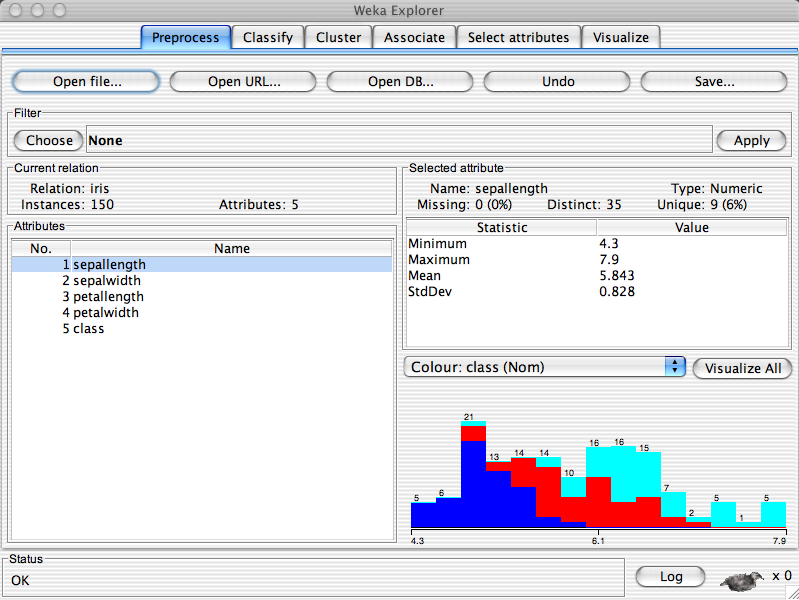
\includegraphics[width=5cm,height=3cm]{weka_2.png}
  \caption[Διεπαφή Weka για προ επεξεργασία δεδομένων]{Διεπαφή Weka: Ο χρήστης παρατηρεί την κατανομή των τιμών ενός χαρακτηριστικού σε 3 διαφορετικές κλάσεις κατά τη προεπεξεργασία.}
  \label{fig:test2}\par\vfill
  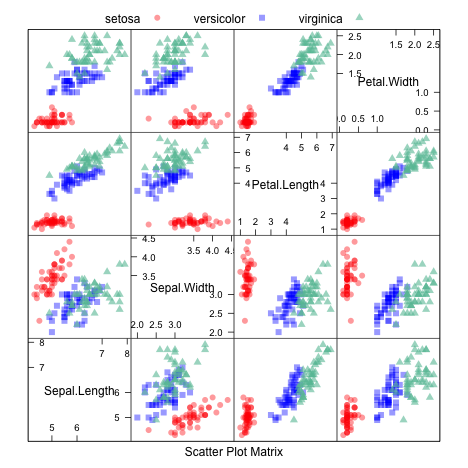
\includegraphics[width=5cm,height=3cm]{caret_2.png}
  \caption[Οπτικοποιήση με το πακέτο Caret]{Το πακέτο Caret παρέχει διάφορα εργαλεία οπτικοποίησης των δεδομένων, όπως διαγράμματα διασποράς. }
  \label{fig:test3}
\end{minipage}
\begin{minipage}[c][11cm][t]{\textwidth}
  \centering
  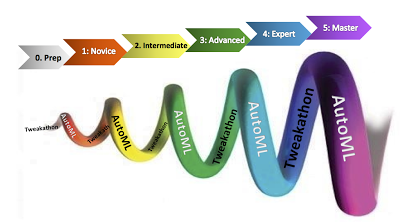
\includegraphics[width=0.8\textwidth,height=4.5cm]{automl_1.png}
  \caption[ChaLearn AutoML challenge ]{ChaLearn AutoML challenge : Η ομάδα ChaLearn διοργανώνει ένα διαγωνισμό μηχανικής μάθησης, όπου οι συμμετέχοντες δοκιμάζονται στη βελτιστοποίηση μοντέλων πρόβλεψης. Μαζί με hackathons και workshops, που διοργανώνονται σε συνεργασία με την Ερευνητική Ομάδα σε Εκπαίδευση, Βελτιστοποίηση και Αυτοματοποίηση του Σχεδιασμού Αλγορίθμων, του Πανεπιστημίου του Freiburg, το γεγονός αυτό συγκεντρώνει και οργανώνει την επιστημονική κοινότητα βοηθώντας στην εξέλιξη της επιστήμης του automl. }
  \label{fig:test2}\par\vfill
\end{minipage}
\end{figure}
\pagestyle{empty}
\begin{thebibliography}{9}

\bibitem{bayesiantutorial} 
Eric Brochu, Vlad M. Cora, Nando de Freitas.
\textit{A Tutorial on Bayesian Optimization of
Expensive Cost Functions, with Application to
Active User Modeling and Hierarchical
Reinforcement Learning}. 
Cornell University Library, Δεκέμβριος 14, 2010.

 \bibitem{wrappers} 
Ron Kohavi, George H. John.
\textit{Wrappers for feature subset selection}. 
14ο Εθνικό Συνέδριο Τεχνητής Νοημοσύνης, Σεπτέμβριος 1995.

 \bibitem{permute} 
Phillip Taylor, Nathan Griffiths, Abhir Bhalerao.
\textit{Redundant Feature Selection using Permutation Methods}. 
ICML  AutoML Workshop, 2014

\bibitem{permute2} 
André Altmann,Laura Toloşi, Oliver Sander, Thomas Lengauer.
\textit{Permutation importance: a corrected feature importance measure}. 
Bioinformatics- Oxford Journal, March 2010

\bibitem{autoweka} 
Chris Thornton, Frank Hutter, Holger H. Hoos, Kevin Leyton-Brown.
\textit{Auto-WEKA: Combined Selection and Hyperparameter
Optimization of Classification Algorithms
}. 
19th ACM SIGKDD international conference on Knowledge discovery and data mining, 2013

\bibitem{hyperpot} 
James Bergstra, Yoshua Bengio, Remi Bardenet, Balazs Kegl
\textit{Algorithms for Hyper-Parameter Optimization}. 

\bibitem{practicalbayes} 
Jasper Snoek, Hugo Larochelle, Ryan P. Adams.
\textit{Practical Bayesian Optimization of Machine
Learning Algorithms}. 
Ιούνιος 2012 


\bibitem{smbo} 
Frank Hutter, Holger H. Hoos, Kevin Leyton-Brown.
\textit{Sequential Model-Based Optimization for
General Algorithm Configuration}. 
Learning and Intelligent Optimization, 5th International Conference, LION 5, Rome, Italy, Ιανουάριος 17-21, 2011

\bibitem{smbo} 
Anil K. Jain, Richard C. Dubes, Chaur-Chin Chen.
\textit{Bootstrap Techniques for Error Estimation}. 
IEEE Transactions on Pattern Analysis and Machine Intelligence, VOL. PAMI-9, NO. 5, Σεπτέμβριος 1987

\bibitem{smbo} 
Jon Shlens.
\textit{A TUTORIAL ON PRINCIPAL COMPONENT ANALYSIS, Derivation, Discussion and Singular Value Decomposition}. 
25 Μαρτίου 2003

\bibitem{smbo} 
Ian H. Witten, Eibe Frank, Mark A. Hall. 
\textit{DATA MINING: Practical Machine Learning Tools and Techniques, 3rd Edition }. 
25 Μαρτίου 2003

\bibitem{caltech} 
Yaser S. Abu-Mustafa.
\textit{Machine Learning online course: Learning from data}. 
Caltech University, 2012

\bibitem{parzenwebsite} 
Parzen-Window Density Estimation.
\url{http://www.cs.utah.edu/~suyash/Dissertation_html/node11.html}

\bibitem{bootwebsite} 
Cross-Validation Vs Bootstrapping .
\url{file:///C:/Users/UserPc1/Downloads/lec27-bootstrap-3.pdf}

\bibitem{mlwebsite} 
Machine Learning Mastery, Discover Feature Engineering, How to Engineer Features and How to Get Good at It
\url{http://machinelearningmastery.com/discover-feature-engineering-how-to-engineer-features-and-how-to-get-good-at-it/}

\bibitem{imbalancewebsite} 
Class Imbalance Problem
\url{http://www.chioka.in/class-imbalance-problem/}

\bibitem{bayes} 
Matthew W. Hoffman.
\textit{Bayesian optimization for automatic machine
learning}. 
ICML  AutoML Workshop, 2015 

\bibitem{caretwebsite} 
The Caret Package
\url{http://topepo.github.io/caret/index.html}

\bibitem{knnwebsite} 
Machine Learning Mastery, K-Nearest Neighbors for Machine Learning
\url{http://machinelearningmastery.com/k-nearest-neighbors-for-machine-learning/}

\bibitem{historywebsite} 
Automated Machine Learning: A Short History.
\url{https://www.datarobot.com/blog/automated-machine-learning-short-history/}
\end{thebibliography}
\end{document}